% Template for PLoS
%DIF LATEXDIFF DIFFERENCE FILE
%DIF DEL cbea.tex           Tue Nov 30 11:48:00 2021
%DIF ADD cbea_revised.tex   Tue Feb  1 18:07:43 2022
% Version 3.5 March 2018
%
% % % % % % % % % % % % % % % % % % % % % %
%
% -- IMPORTANT NOTE
%
% This template contains comments intended 
% to minimize problems and delays during our production 
% process. Please follow the template instructions
% whenever possible.
%
% % % % % % % % % % % % % % % % % % % % % % % 
%
% Once your paper is accepted for publication, 
% PLEASE REMOVE ALL TRACKED CHANGES in this file 
% and leave only the final text of your manuscript. 
% PLOS recommends the use of latexdiff to track changes during review, as this will help to maintain a clean tex file.
% Visit https://www.ctan.org/pkg/latexdiff?lang=en for info or contact us at latex@plos.org.
%
%
% There are no restrictions on package use within the LaTeX files except that 
% no packages listed in the template may be deleted.
%
% Please do not include colors or graphics in the text.
%
% The manuscript LaTeX source should be contained within a single file (do not use \input, \externaldocument, or similar commands).
%
% % % % % % % % % % % % % % % % % % % % % % %
%
% -- FIGURES AND TABLES
%
% Please include tables/figure captions directly after the paragraph where they are first cited in the text.
%
% DO NOT INCLUDE GRAPHICS IN YOUR MANUSCRIPT
% - Figures should be uploaded separately from your manuscript file. 
% - Figures generated using LaTeX should be extracted and removed from the PDF before submission. 
% - Figures containing multiple panels/subfigures must be combined into one image file before submission.
% For figure citations, please use "Fig" instead of "Figure".
% See http://journals.plos.org/plosone/s/figures for PLOS figure guidelines.
%
% Tables should be cell-based and may not contain:
% - spacing/line breaks within cells to alter layout or alignment
% - do not nest tabular environments (no tabular environments within tabular environments)
% - no graphics or colored text (cell background color/shading OK)
% See http://journals.plos.org/plosone/s/tables for table guidelines.
%
% For tables that exceed the width of the text column, use the adjustwidth environment as illustrated in the example table in text below.
%
% % % % % % % % % % % % % % % % % % % % % % % %
%
% -- EQUATIONS, MATH SYMBOLS, SUBSCRIPTS, AND SUPERSCRIPTS
%
% IMPORTANT
% Below are a few tips to help format your equations and other special characters according to our specifications. For more tips to help reduce the possibility of formatting errors during conversion, please see our LaTeX guidelines at http://journals.plos.org/plosone/s/latex
%
% For inline equations, please be sure to include all portions of an equation in the math environment.  For example, x$^2$ is incorrect; this should be formatted as $x^2$ (or $\mathrm{x}^2$ if the romanized font is desired).
%
% Do not include text that is not math in the math environment. For example, CO2 should be written as CO\textsubscript{2} instead of CO$_2$.
%
% Please add line breaks to long display equations when possible in order to fit size of the column. 
%
% For inline equations, please do not include punctuation (commas, etc) within the math environment unless this is part of the equation.
%
% When adding superscript or subscripts outside of brackets/braces, please group using {}.  For example, change "[U(D,E,\gamma)]^2" to "{[U(D,E,\gamma)]}^2". 
%
% Do not use \cal for caligraphic font.  Instead, use \mathcal{}
%
% % % % % % % % % % % % % % % % % % % % % % % % 
%
% Please contact latex@plos.org with any questions.
%
% % % % % % % % % % % % % % % % % % % % % % % %

\documentclass[10pt,letterpaper]{article}
\usepackage[top=0.85in,left=2.75in,footskip=0.75in]{geometry}

% amsmath and amssymb packages, useful for mathematical formulas and symbols
\usepackage{amsmath,amssymb}

% Use adjustwidth environment to exceed column width (see example table in text)
\usepackage{changepage}

% Use Unicode characters when possible
\usepackage[utf8x]{inputenc}

% textcomp package and marvosym package for additional characters
\usepackage{textcomp,marvosym}

% cite package, to clean up citations in the main text. Do not remove.
\usepackage{cite}

% Use nameref to cite supporting information files (see Supporting Information section for more info)
\usepackage{nameref,hyperref}

% line numbers
\usepackage[right]{lineno}

% ligatures disabled
\usepackage{microtype}
\DisableLigatures[f]{encoding = *, family = * }

% color can be used to apply background shading to table cells only
\usepackage[table]{xcolor}

% array package and thick rules for tables
\usepackage{array}

% create "+" rule type for thick vertical lines
\newcolumntype{+}{!{\vrule width 2pt}}

% create \thickcline for thick horizontal lines of variable length
\newlength\savedwidth
\newcommand\thickcline[1]{%
  \noalign{\global\savedwidth\arrayrulewidth\global\arrayrulewidth 2pt}%
  \cline{#1}%
  \noalign{\vskip\arrayrulewidth}%
  \noalign{\global\arrayrulewidth\savedwidth}%
}

% \thickhline command for thick horizontal lines that span the table
\newcommand\thickhline{\noalign{\global\savedwidth\arrayrulewidth\global\arrayrulewidth 2pt}%
\hline
\noalign{\global\arrayrulewidth\savedwidth}}


% Remove comment for double spacing
%\usepackage{setspace} 
%\doublespacing

% Text layout
\raggedright
\setlength{\parindent}{0.5cm}
\textwidth 5.25in 
\textheight 8.75in

% Bold the 'Figure #' in the caption and separate it from the title/caption with a period
% Captions will be left justified
\usepackage[aboveskip=1pt,labelfont=bf,labelsep=period,justification=raggedright,singlelinecheck=off]{caption}
\renewcommand{\figurename}{Fig}

% Use the PLoS provided BiBTeX style
\bibliographystyle{plos2015}

% Remove brackets from numbering in List of References
\makeatletter
\renewcommand{\@biblabel}[1]{\quad#1.}
\makeatother



% Header and Footer with logo
\usepackage{lastpage,fancyhdr,graphicx}
\usepackage{epstopdf}
%\pagestyle{myheadings}
\pagestyle{fancy}
\fancyhf{}
%\setlength{\headheight}{27.023pt}
%\lhead{\includegraphics[width=2.0in]{PLOS-submission.eps}}
\rfoot{\thepage/\pageref{LastPage}}
\renewcommand{\headrulewidth}{0pt}
\renewcommand{\footrule}{\hrule height 2pt \vspace{2mm}}
\fancyheadoffset[L]{2.25in}
\fancyfootoffset[L]{2.25in}
\lfoot{\today}

%% Include all macros below

\newcommand{\lorem}{{\bf LOREM}}
\newcommand{\ipsum}{{\bf IPSUM}}

%% END MACROS SECTION

% Adding packages 
\usepackage{bm}
\usepackage[parfill]{parskip}
\usepackage{float} %DIF > 
 %DIF > 
% Adding overline macro  %DIF > 
\newcommand{\overbar}[1]{\mkern 2mu\overline{\mkern-2mu#1\mkern-20mu}\mkern 20mu} %DIF > 
%DIF PREAMBLE EXTENSION ADDED BY LATEXDIFF
%DIF UNDERLINE PREAMBLE %DIF PREAMBLE
\RequirePackage[normalem]{ulem} %DIF PREAMBLE
\RequirePackage{color}\definecolor{RED}{rgb}{1,0,0}\definecolor{BLUE}{rgb}{0,0,1} %DIF PREAMBLE
\providecommand{\DIFaddtex}[1]{{\protect\color{blue}\uwave{#1}}} %DIF PREAMBLE
\providecommand{\DIFdeltex}[1]{{\protect\color{red}\sout{#1}}}                      %DIF PREAMBLE
%DIF SAFE PREAMBLE %DIF PREAMBLE
\providecommand{\DIFaddbegin}{} %DIF PREAMBLE
\providecommand{\DIFaddend}{} %DIF PREAMBLE
\providecommand{\DIFdelbegin}{} %DIF PREAMBLE
\providecommand{\DIFdelend}{} %DIF PREAMBLE
\providecommand{\DIFmodbegin}{} %DIF PREAMBLE
\providecommand{\DIFmodend}{} %DIF PREAMBLE
%DIF FLOATSAFE PREAMBLE %DIF PREAMBLE
\providecommand{\DIFaddFL}[1]{\DIFadd{#1}} %DIF PREAMBLE
\providecommand{\DIFdelFL}[1]{\DIFdel{#1}} %DIF PREAMBLE
\providecommand{\DIFaddbeginFL}{} %DIF PREAMBLE
\providecommand{\DIFaddendFL}{} %DIF PREAMBLE
\providecommand{\DIFdelbeginFL}{} %DIF PREAMBLE
\providecommand{\DIFdelendFL}{} %DIF PREAMBLE
%DIF HYPERREF PREAMBLE %DIF PREAMBLE
\providecommand{\DIFadd}[1]{\texorpdfstring{\DIFaddtex{#1}}{#1}} %DIF PREAMBLE
\providecommand{\DIFdel}[1]{\texorpdfstring{\DIFdeltex{#1}}{}} %DIF PREAMBLE
\newcommand{\DIFscaledelfig}{0.5}
%DIF HIGHLIGHTGRAPHICS PREAMBLE %DIF PREAMBLE
\RequirePackage{settobox} %DIF PREAMBLE
\RequirePackage{letltxmacro} %DIF PREAMBLE
\newsavebox{\DIFdelgraphicsbox} %DIF PREAMBLE
\newlength{\DIFdelgraphicswidth} %DIF PREAMBLE
\newlength{\DIFdelgraphicsheight} %DIF PREAMBLE
% store original definition of \includegraphics %DIF PREAMBLE
\LetLtxMacro{\DIFOincludegraphics}{\includegraphics} %DIF PREAMBLE
\newcommand{\DIFaddincludegraphics}[2][]{{\color{blue}\fbox{\DIFOincludegraphics[#1]{#2}}}} %DIF PREAMBLE
\newcommand{\DIFdelincludegraphics}[2][]{% %DIF PREAMBLE
\sbox{\DIFdelgraphicsbox}{\DIFOincludegraphics[#1]{#2}}% %DIF PREAMBLE
\settoboxwidth{\DIFdelgraphicswidth}{\DIFdelgraphicsbox} %DIF PREAMBLE
\settoboxtotalheight{\DIFdelgraphicsheight}{\DIFdelgraphicsbox} %DIF PREAMBLE
\scalebox{\DIFscaledelfig}{% %DIF PREAMBLE
\parbox[b]{\DIFdelgraphicswidth}{\usebox{\DIFdelgraphicsbox}\\[-\baselineskip] \rule{\DIFdelgraphicswidth}{0em}}\llap{\resizebox{\DIFdelgraphicswidth}{\DIFdelgraphicsheight}{% %DIF PREAMBLE
\setlength{\unitlength}{\DIFdelgraphicswidth}% %DIF PREAMBLE
\begin{picture}(1,1)% %DIF PREAMBLE
\thicklines\linethickness{2pt} %DIF PREAMBLE
{\color[rgb]{1,0,0}\put(0,0){\framebox(1,1){}}}% %DIF PREAMBLE
{\color[rgb]{1,0,0}\put(0,0){\line( 1,1){1}}}% %DIF PREAMBLE
{\color[rgb]{1,0,0}\put(0,1){\line(1,-1){1}}}% %DIF PREAMBLE
\end{picture}% %DIF PREAMBLE
}\hspace*{3pt}}} %DIF PREAMBLE
} %DIF PREAMBLE
\LetLtxMacro{\DIFOaddbegin}{\DIFaddbegin} %DIF PREAMBLE
\LetLtxMacro{\DIFOaddend}{\DIFaddend} %DIF PREAMBLE
\LetLtxMacro{\DIFOdelbegin}{\DIFdelbegin} %DIF PREAMBLE
\LetLtxMacro{\DIFOdelend}{\DIFdelend} %DIF PREAMBLE
\DeclareRobustCommand{\DIFaddbegin}{\DIFOaddbegin \let\includegraphics\DIFaddincludegraphics} %DIF PREAMBLE
\DeclareRobustCommand{\DIFaddend}{\DIFOaddend \let\includegraphics\DIFOincludegraphics} %DIF PREAMBLE
\DeclareRobustCommand{\DIFdelbegin}{\DIFOdelbegin \let\includegraphics\DIFdelincludegraphics} %DIF PREAMBLE
\DeclareRobustCommand{\DIFdelend}{\DIFOaddend \let\includegraphics\DIFOincludegraphics} %DIF PREAMBLE
\LetLtxMacro{\DIFOaddbeginFL}{\DIFaddbeginFL} %DIF PREAMBLE
\LetLtxMacro{\DIFOaddendFL}{\DIFaddendFL} %DIF PREAMBLE
\LetLtxMacro{\DIFOdelbeginFL}{\DIFdelbeginFL} %DIF PREAMBLE
\LetLtxMacro{\DIFOdelendFL}{\DIFdelendFL} %DIF PREAMBLE
\DeclareRobustCommand{\DIFaddbeginFL}{\DIFOaddbeginFL \let\includegraphics\DIFaddincludegraphics} %DIF PREAMBLE
\DeclareRobustCommand{\DIFaddendFL}{\DIFOaddendFL \let\includegraphics\DIFOincludegraphics} %DIF PREAMBLE
\DeclareRobustCommand{\DIFdelbeginFL}{\DIFOdelbeginFL \let\includegraphics\DIFdelincludegraphics} %DIF PREAMBLE
\DeclareRobustCommand{\DIFdelendFL}{\DIFOaddendFL \let\includegraphics\DIFOincludegraphics} %DIF PREAMBLE
%DIF LISTINGS PREAMBLE %DIF PREAMBLE
\RequirePackage{listings} %DIF PREAMBLE
\RequirePackage{color} %DIF PREAMBLE
\lstdefinelanguage{DIFcode}{ %DIF PREAMBLE
%DIF DIFCODE_UNDERLINE %DIF PREAMBLE
  moredelim=[il][\color{red}\sout]{\%DIF\ <\ }, %DIF PREAMBLE
  moredelim=[il][\color{blue}\uwave]{\%DIF\ >\ } %DIF PREAMBLE
} %DIF PREAMBLE
\lstdefinestyle{DIFverbatimstyle}{ %DIF PREAMBLE
	language=DIFcode, %DIF PREAMBLE
	basicstyle=\ttfamily, %DIF PREAMBLE
	columns=fullflexible, %DIF PREAMBLE
	keepspaces=true %DIF PREAMBLE
} %DIF PREAMBLE
\lstnewenvironment{DIFverbatim}{\lstset{style=DIFverbatimstyle}}{} %DIF PREAMBLE
\lstnewenvironment{DIFverbatim*}{\lstset{style=DIFverbatimstyle,showspaces=true}}{} %DIF PREAMBLE
%DIF END PREAMBLE EXTENSION ADDED BY LATEXDIFF

\begin{document}
\vspace*{0.2in}

% Title must be 250 characters or less.
\begin{flushleft}
{\Large
\textbf\DIFdelbegin %DIFDELCMD < \newline{cILR: Competitive isometric log-ratio for taxonomic enrichment analysis} %%%
\DIFdelend \DIFaddbegin \newline{CBEA: Competitive balances for taxonomic enrichment analysis} \DIFaddend % Please use "sentence case" for title and headings (capitalize only the first word in a title (or heading), the first word in a subtitle (or subheading), and any proper nouns).
}
\newline
% Insert author names, affiliations and corresponding author email (do not include titles, positions, or degrees).
\\
Quang P. Nguyen\textsuperscript{1,2},
Anne G. Hoen\textsuperscript{1,2\ddag},
H. Robert Frost\textsuperscript{1*\ddag\dag},
\\
\bigskip
\textbf{1} Department of Biomedical Data Science, Geisel School of Medicine at Dartmouth College, Hanover, NH, USA
\\
\textbf{2} Department of Epidemiology, Geisel School of Medicine at Dartmouth College, Hanover, NH, USA
\\
\bigskip

% Insert additional author notes using the symbols described below. Insert symbol callouts after author names as necessary.
% 
% Remove or comment out the author notes below if they aren't used.
%
% Primary Equal Contribution Note
%\Yinyang These authors contributed equally to this work.

% Additional Equal Contribution Note
% Also use this double-dagger symbol for special authorship notes, such as senior authorship.
\ddag These authors jointly supervised this work.\\
\dag Corresponding author
% Current address notes
%\textcurrency Current Address: Dept/Program/Center, Institution Name, City, State, Country % change symbol to "\textcurrency a" if more than one current address note
% \textcurrency b Insert second current address 
% \textcurrency c Insert third current address

% Deceased author note
% \dag Deceased

% Group/Consortium Author Note
%\textpilcrow Membership list can be found in the Acknowledgments section.

% Use the asterisk to denote corresponding authorship and provide email address in note below.
* hildreth.r.frost@dartmouth.edu

\end{flushleft}
% Please keep the abstract below 300 words
\section*{Abstract}
Research in human associated microbiomes often involves the analysis of taxonomic count tables generated via high-throughput sequencing. It is difficult to apply statistical tools as the data is high-dimensional, sparse, and \DIFdelbegin \DIFdel{strictly }\DIFdelend compositional. An approachable way to alleviate high-dimensionality and sparsity is to aggregate variables into pre-defined sets. Set-based analysis is ubiquitous in the genomics literature, and has demonstrable impact in improving interpretability and power of downstream analysis. Unfortunately, there is a lack of sophisticated set-based analysis methods specific to microbiome taxonomic data, where current practice often employs abundance summation as a technique for aggregation. This approach prevents comparison across sets of different sizes, does not preserve inter-sample distances, and amplifies protocol bias. Here, we attempt to fill this gap with a new single sample taxon \DIFdelbegin \DIFdel{set enrichment method }\DIFdelend \DIFaddbegin \DIFadd{enrichment method with using a novel log-ratio formulation }\DIFaddend based on the \DIFdelbegin \DIFdel{isometric log ratio transformation and the }\DIFdelend competitive null hypothesis commonly used in the enrichment analysis literature. Our approach, titled competitive \DIFdelbegin \DIFdel{isometric log ratio (cILR}\DIFdelend \DIFaddbegin \DIFadd{balances for taxonomic enrichment analysis (CBEA}\DIFaddend ), generates sample-specific enrichment scores as the scaled log ratio of the subcomposition defined by taxa within a set and the subcomposition defined by its complement. We provide sample-level significance testing by estimating an empirical null distribution of our test statistic with valid p-values. Herein we demonstrate using both real data applications and simulations that \DIFdelbegin \DIFdel{cILR }\DIFdelend \DIFaddbegin \DIFadd{CBEA }\DIFaddend controls for type I error even under high sparsity and high inter-taxa correlation scenarios. Additionally, it provides informative scores that can be inputs to downstream \DIFdelbegin \DIFdel{differential abundance and }\DIFdelend \DIFaddbegin \DIFadd{analyses such as }\DIFaddend prediction tasks. 


% Please keep the Author Summary between 150 and 200 words
% Use first person. PLOS ONE authors please skip this step. 
% Author Summary not valid for PLOS ONE submissions.   
\section*{Author summary}
The study of human associated microbiomes relies on genomic surveys via high-throughput sequencing. However, microbiome taxonomic data is sparse and high dimensional which prevents the application of standard statistical techniques. One approach to address this problem is to perform analyses at the level of taxon sets. Set-based analysis has a long history in the genomics literature, with demonstrable impact in improving both power and interpretability. Unfortunately, there is not a lot of research in developing new set-based tools for microbiome taxonomic data specifically, given \DIFdelbegin \DIFdel{that }\DIFdelend \DIFaddbegin \DIFadd{its unique features }\DIFaddend compared to other 'omics data types\DIFdelbegin \DIFdel{microbiome taxonomic data is strictly compositional}\DIFdelend . We developed a new tool to generate taxon set enrichment scores at the sample level \DIFdelbegin \DIFdel{by combining the isometric }\DIFdelend \DIFaddbegin \DIFadd{through a novel }\DIFaddend log-ratio \DIFdelbegin \DIFdel{and }\DIFdelend \DIFaddbegin \DIFadd{formulation based on }\DIFaddend the competitive null hypothesis. Our scores can be used for statistical inference \DIFdelbegin \DIFdel{, and as }\DIFdelend \DIFaddbegin \DIFadd{at both the sample and population levels, as well as }\DIFaddend inputs to other downstream analyses such as \DIFdelbegin \DIFdel{differential abundance and }\DIFdelend prediction models. We demonstrate the performance of our method against competing approaches across both real data analyses and simulation studies. 

\linenumbers

% Use "Eq" instead of "Equation" for equation citations.
\section*{Introduction} \DIFaddbegin \label{introduction}
\DIFaddend The microbiome is the collection of microorganisms (bacteria, protozoa, archaea, fungi, and viruses) which co-exist with their host. Previous research has shown that changes in the composition of the human gut microbiome are associated with important health outcomes such as inflammatory bowel disease \cite{proctor2019}, type II diabetes \DIFdelbegin \DIFdel{\mbox{%DIFAUXCMD
\cite{sharma2019}}\hspace{0pt}%DIFAUXCMD
}\DIFdelend \DIFaddbegin \DIFadd{\mbox{%DIFAUXCMD
\cite{sharma2019a}}\hspace{0pt}%DIFAUXCMD
}\DIFaddend , and obesity \cite{aoun2020}. To understand the central role of the microbiome in human health, researchers have relied on high-throughput sequencing methods, either by targeting a specific representative gene (i.e. amplicon sequencing) or by profiling all the genomic content of the sample (i.e. whole-genome shotgun sequencing) \cite{cho2012}. Raw sequencing data is then processed through a variety of bioinformatic pipelines \cite{callahan2016, truong2015}, yielding various data products, one of which are taxonomic tables which can be used to study associations between members of the microbiome and an exposure or outcome of interest. 

However, there exists unique challenges in the analysis of these taxonomic count tables \DIFdelbegin \DIFdel{\mbox{%DIFAUXCMD
\cite{li2019,li2015}}\hspace{0pt}%DIFAUXCMD
. First, like other sequencing-based datasets, microbiome count data is often high dimensional, where the number of detected taxa far exceeds the number of samples usually present. For predictive tasks, microbiome-specific penalized regression approaches have been developed to address this issue \mbox{%DIFAUXCMD
\cite{shi2016}}\hspace{0pt}%DIFAUXCMD
, allowing for simultaneous model fitting and variable selection. For differential abundance tasks, researchers often utilize multiple hypothesis correction methods \mbox{%DIFAUXCMD
\cite{sankaran2014,benjamini1995} }\hspace{0pt}%DIFAUXCMD
or omnibus tests \mbox{%DIFAUXCMD
\cite{chen2018} }\hspace{0pt}%DIFAUXCMD
to address hypothesis testing burden. 
}%DIFDELCMD < 

%DIFDELCMD < %%%
\DIFdel{Second, the number of reads obtained is constrained by the sequencing instrument at an arbitrary limit, and is inconsistent across samples, resulting in a variable number of total read counts per sample. Many normalization methods \mbox{%DIFAUXCMD
\cite{weiss2017} }\hspace{0pt}%DIFAUXCMD
have been proposed to address these issues, including cross-applying methods from the gene expression literature \mbox{%DIFAUXCMD
\cite{mcmurdie2014}}\hspace{0pt}%DIFAUXCMD
. However, these methods rely on assumptions specific to the original bulk RNA-seq data sets such as the presence of housekeeping genes with consistent expression levels \mbox{%DIFAUXCMD
\cite{love2014}}\hspace{0pt}%DIFAUXCMD
, which might not be not true in the context of microbiome relative abundance data \mbox{%DIFAUXCMD
\cite{quinn2019,quinn2018b}}\hspace{0pt}%DIFAUXCMD
. As such, microbiome taxonomic data is strictly compositional \mbox{%DIFAUXCMD
\cite{gloor2017}}\hspace{0pt}%DIFAUXCMD
, which means that the abundance of any taxa can only be interpreted relative to another. Consequently, log-ratio transformations from the compositional data literature are often utilized \mbox{%DIFAUXCMD
\cite{aitchison1999}}\hspace{0pt}%DIFAUXCMD
. 
}%DIFDELCMD < 

%DIFDELCMD < %%%
\DIFdel{Third, the data are highly zero-inflated, where there is a high number of both structural zeros (truly missing due to biological reasons) and sampling zeroes (due to limits of detection of the sequencing experiment). Researchers often dealt with these issues by imputing zero cells with a pseudocount \mbox{%DIFAUXCMD
\cite{kurtz2015}}\hspace{0pt}%DIFAUXCMD
, or applying zero-inflated models \mbox{%DIFAUXCMD
\cite{chen2018, kaul2017}}\hspace{0pt}%DIFAUXCMD
. Newer methods developed recently have focused on understanding the different types of zeros in the data, providing more sophisticated heuristics around when pseudocounts can be utilized \mbox{%DIFAUXCMD
\cite{kaul2017a}}\hspace{0pt}%DIFAUXCMD
.   
}%DIFDELCMD < 

%DIFDELCMD < %%%
\DIFdelend \DIFaddbegin \DIFadd{\mbox{%DIFAUXCMD
\cite{li2019a,li2015}}\hspace{0pt}%DIFAUXCMD
. The data is sparse, high-dimensional, and likely compositional \mbox{%DIFAUXCMD
\cite{gloor2017, li2019a, li2015}}\hspace{0pt}%DIFAUXCMD
. }\DIFaddend Even though the \DIFdelbegin \DIFdel{aforementioned }\DIFdelend \DIFaddbegin \DIFadd{these }\DIFaddend problems are challenging, a very approachable \DIFdelbegin \DIFdel{method to address some of them is through }\DIFdelend \DIFaddbegin \DIFadd{solution is to to use }\DIFaddend set-based analysis \DIFaddbegin \DIFadd{methods}\DIFaddend , also termed gene set testing in the genomics literature \cite{khatri2012, goeman2007}. Aggregated \DIFdelbegin \DIFdel{sets are less sparsethan their constituent elements}\DIFdelend \DIFaddbegin \DIFadd{variables can be less sparse}\DIFaddend , and testing on a smaller number of \DIFdelbegin \DIFdel{variables reduces the multiple testing burden, thereby increasing }\DIFdelend \DIFaddbegin \DIFadd{features can reduce the multiple-testing burden. As such, gene set testing methods have been shown to increase }\DIFaddend power and reproducibility \DIFdelbegin \DIFdel{. Through }\DIFdelend \DIFaddbegin \DIFadd{of genomic analyses. Furthermore, through }\DIFaddend the usage of functionally informative sets defined apriori based on historical experiments (for example MSigDB \cite{subramanian2005}, and Gene Ontology \cite{ashburner2000}), gene set \DIFdelbegin \DIFdel{analyses }\DIFdelend \DIFaddbegin \DIFadd{analysis }\DIFaddend also allows for more \DIFaddbegin \DIFadd{biologically }\DIFaddend informative interpretations. 
\DIFaddbegin 

\DIFaddend There exists a diverse set of \DIFdelbegin \DIFdel{available methods developed to perform such analyses. More traditional set testing }\DIFdelend methods \DIFaddbegin \DIFadd{already developed in this field. Traditional methods }\DIFaddend utilize the hypergeometric \DIFdelbegin \DIFdel{test }\DIFdelend \DIFaddbegin \DIFadd{distribution }\DIFaddend to test for the overrepresentation of \DIFdelbegin \DIFdel{significant p-values for a set of interest }\DIFdelend \DIFaddbegin \DIFadd{a gene set using a candidate list of genes screened based on a marginal model }\DIFaddend \cite{goeman2007}. Unfortunately, these approaches are sensitive to the differential expression test \DIFdelbegin \DIFdel{and their generated p-values. The most widely used gene-set analysis method, GSEA \mbox{%DIFAUXCMD
\cite{subramanian2005}}\hspace{0pt}%DIFAUXCMD
, instead uses a random-walk-like statistic through a ranking of genes based on a measure of association or effect size. Both of these methods generate enrichment scores and significance testing }\DIFdelend \DIFaddbegin \DIFadd{as well as the chosen threshold when trying to select genes for the candidate list. Aggregate score methods, which are generally more preferred \mbox{%DIFAUXCMD
\cite{irizarry2009}}\hspace{0pt}%DIFAUXCMD
, instead assigns a score for each gene set based on gene-specific statistics such as z-scores or fold change. Of these approaches, methods such as GSEA \mbox{%DIFAUXCMD
\cite{subramanian2005} }\hspace{0pt}%DIFAUXCMD
performs a test for each gene set }\DIFaddend at the population level, \DIFdelbegin \DIFdel{incorporating information from }\DIFdelend \DIFaddbegin \DIFadd{summarizing information across }\DIFaddend all samples. Conversely, methods such as GSVA \cite{hanzelmann2013} and VAM \DIFdelbegin \DIFdel{\mbox{%DIFAUXCMD
\cite{frost2020a}}\hspace{0pt}%DIFAUXCMD
}\DIFdelend \DIFaddbegin \DIFadd{\mbox{%DIFAUXCMD
\cite{frost2020}}\hspace{0pt}%DIFAUXCMD
}\DIFaddend , generate enrichment scores at the sample level and are more akin to a transformation. \DIFdelbegin \DIFdel{This strategy }\DIFdelend \DIFaddbegin \DIFadd{In addition to being able to screen for enriched sets per sample, this strategy also }\DIFaddend allows for the flexible incorporation of different \DIFdelbegin \DIFdel{statistical techniques downstream }\DIFdelend \DIFaddbegin \DIFadd{downstream analyses}\DIFaddend , such as \DIFaddbegin \DIFadd{fitting }\DIFaddend prediction models, \DIFdelbegin \DIFdel{as well as for visualization purposes in ordination plots}\DIFdelend \DIFaddbegin \DIFadd{or performing dimension reduction}\DIFaddend .  

%DIF > First, like other sequencing-based datasets, microbiome count data is often high dimensional, where the number of detected taxa far exceeds the number of samples usually present. For predictive tasks, microbiome-specific penalized regression approaches have been developed to address this issue \cite{shi2016a}, allowing for simultaneous model fitting and variable selection. For differential abundance tasks, researchers often utilize multiple hypothesis correction methods \cite{sankaran2014,benjamini1995} or omnibus tests \cite{chen2018c} to address hypothesis testing burden. 
\DIFaddbegin 

%DIF > Second, the total number of reads varies across samples due to limitations of the sequencing instrument \cite{quinn2018}. 

%DIF > Third, the data are highly sparse, where there is a high number of both structural zeros (truly missing due to biological reasons) and sampling zeroes (due to limits of detection of the sequencing experiment). Researchers often dealt with these issues by imputing zero cells with a pseudocount \cite{kurtz2015a}, or applying zero-inflated models \cite{chen2018c, kaul2017}. Newer methods developed recently have focused on understanding the different types of zeros in the data, providing more sophisticated heuristics around when pseudocounts can be utilized \cite{kaul2017a}.   

\DIFaddend In microbiome research, even though no explicit enrichment analysis is performed, \DIFdelbegin \DIFdel{standard practice often involves aggregating }\DIFdelend \DIFaddbegin \DIFadd{researchers often aggregate }\DIFaddend taxa to higher Linnean classification levels such as genus, family, or phylum\DIFdelbegin \DIFdel{by simple summation of abundances \mbox{%DIFAUXCMD
\cite{mclaren2019}}\hspace{0pt}%DIFAUXCMD
. Even though this allows for a reduction in the number of overall taxa (from thousands to only hundreds), there still exist three disadvantages: first, inter-sample distances are not preserved before and after aggregation \mbox{%DIFAUXCMD
\cite{egozcue2005}}\hspace{0pt}%DIFAUXCMD
, second, it doesn't allow for enrichment testing and comparison across sets of different sizes, and third, it increases bias when taxa within the set have different efficiencies in how they are measured through sequencing \mbox{%DIFAUXCMD
\cite{mclaren2019}}\hspace{0pt}%DIFAUXCMD
. As such, there is a need for microbiome researchers to adopt more robust sample-level set enrichment methods. Unfortunately, limited work has been }\DIFdelend \DIFaddbegin \DIFadd{. However, despite this interest, there is limited research }\DIFaddend done to extend existing \DIFdelbegin \DIFdel{methods to be more specific to }\DIFdelend \DIFaddbegin \DIFadd{set-based methods to }\DIFaddend microbiome relative abundance data. Some software suites, such as \emph{MicrobiomeAnalyst}, do offer tools to perform enrichment testing with curated taxon sets \cite{chong2020}. However, the approach used in \emph{MicrobiomeAnalyst} is a form of overrepresentation analysis at the population level and therefore similarly sensitive to the differential abundance approach used \DIFdelbegin \DIFdel{. 
}\DIFdelend \DIFaddbegin \DIFadd{and p-value threshold. One of the primary challenges for adapting gene set analysis to the microbiome context is the compositional nature of the data. Sequencing technologies constrain the total number of reads, and samples are expected to have the same number of reads instead of DNA content \mbox{%DIFAUXCMD
\cite{quinn2019, quinn2018}}\hspace{0pt}%DIFAUXCMD
. However, different samples still yield arbitrarily different total read counts \mbox{%DIFAUXCMD
\cite{morton2019, gloor2017}}\hspace{0pt}%DIFAUXCMD
, suggesting the use of normalization methods to allow for proper comparison of feature abundances across samples. However, microbiome data sets do not follow certain assumptions that enable the cross-application of methods from similar fields (such as RNA-seq) \mbox{%DIFAUXCMD
\cite{quinn2019, quinn2018}}\hspace{0pt}%DIFAUXCMD
. For example, DESeq2's }\emph{\DIFadd{estimateSizeFactors}} \DIFadd{\mbox{%DIFAUXCMD
\cite{love2014} }\hspace{0pt}%DIFAUXCMD
assumes that the majority of genes acts as housekeeping genes with constant expression levels across samples. As such, practitioners often rely on total sum normalization to transform count data into relative proportions that sum to one \mbox{%DIFAUXCMD
\cite{weiss2017}}\hspace{0pt}%DIFAUXCMD
. Some studies have provided emprical performance vealuations supporting this normalization schema \mbox{%DIFAUXCMD
\cite{mcknight2019}}\hspace{0pt}%DIFAUXCMD
. Since this approach imposes a sum constraint on the data, post normalization microbiome data sets are compositional \mbox{%DIFAUXCMD
\cite{gloor2017}}\hspace{0pt}%DIFAUXCMD
, which means that the abundance of any taxa can only be interpreted relative to another. Under this scenario, log-ratio based approaches from the compositional data analysis (CoDA) literature \mbox{%DIFAUXCMD
\cite{aitchison1994} }\hspace{0pt}%DIFAUXCMD
are motivated to address this issue. 
}\DIFaddend 

\DIFaddbegin \DIFadd{Unfortunately, the standard practice for aggregating variables using element-wise summations (referred to as amalgamations in the CoDA literature), does not adequately address the compositional issue \mbox{%DIFAUXCMD
\cite{mclaren2019}}\hspace{0pt}%DIFAUXCMD
. First, inter-sample Aitchison distances computed on original parts are not preserved after amalgamation \mbox{%DIFAUXCMD
\cite{egozcue2005}}\hspace{0pt}%DIFAUXCMD
. This means that cluster analyses might show different results depending on the level of amalgamation and differs from the those computed from original variables. Second, amalgamations do not allow for comparison between sets of different sizes within the same experimental condition since larger sets will have larger means and variances. Third, considering that each taxa has specific measurement biases \mbox{%DIFAUXCMD
\cite{mclaren2019}}\hspace{0pt}%DIFAUXCMD
, an amalgamation based approach would make the bias of the amalgamated variable dependent on the relative abundance of the its constituents. In other words, if taxon $1$ has abundance $A_1$ and bias $B_1$, while taxon $2$ has abundance $A_2$ and bias $B_2$, then the bias of the aggregate variable (for example, a genera) is $(A_1B_1 + A_2B_2)/(A_1 + A_2)$ (see Appendix 1. from McLaren et al. \mbox{%DIFAUXCMD
\cite{mclaren2019}}\hspace{0pt}%DIFAUXCMD
). This means that bias invariant approaches (such as analyses of ratios) would no longer be invariant when applied to amalgamated variables as bias now varies across samples. The alternative would be to multiply the proportions rather than to sum them \mbox{%DIFAUXCMD
\cite{egozcue2005}}\hspace{0pt}%DIFAUXCMD
. 
}

\DIFaddend Here, we present a \DIFdelbegin \DIFdel{novel method that }\DIFdelend \DIFaddbegin \DIFadd{taxon-set testing method for microbiome relative abundance data that addresses the aforementioned issues. Our approach }\DIFaddend generates enrichment scores at the sample level similar to GSVA \cite{hanzelmann2013} and VAM \DIFdelbegin \DIFdel{\mbox{%DIFAUXCMD
\cite{frost2020a}}\hspace{0pt}%DIFAUXCMD
}\DIFdelend \DIFaddbegin \DIFadd{\mbox{%DIFAUXCMD
\cite{frost2020}}\hspace{0pt}%DIFAUXCMD
}\DIFaddend . We leverage the concept of the $Q_1$ competitive hypothesis presented in Tian et al. \cite{tian2005} \DIFdelbegin \DIFdel{, which tests the null that the value of variables within a specific set is equal to the value of measured variables not in the set . The competitive null hypothesis is particularly useful in compositional data analysis, as it naturally assesses enrichment as a ratio between two sets of variables. We incorporated this insight with the isometric log-ratio transformation \mbox{%DIFAUXCMD
\cite{egozcue2003}}\hspace{0pt}%DIFAUXCMD
, which allows for a multiplicative aggregation method that addresses the downsides of the naive summation-based method presented above \mbox{%DIFAUXCMD
\cite{mclaren2019, silverman2017}}\hspace{0pt}%DIFAUXCMD
. The resulting method, titled competitive isometric log-ratio (cILR), is therefore unsupervised and can generate sample-specific enrichment scores with a }\DIFdelend \DIFaddbegin \DIFadd{to formulate the enrichment of a set as the compositional balance \mbox{%DIFAUXCMD
\cite{rivera-pinto2018} }\hspace{0pt}%DIFAUXCMD
of taxa within the set and remainder taxa using multiplication as the method of aggregating proportions \mbox{%DIFAUXCMD
\cite{egozcue2005}}\hspace{0pt}%DIFAUXCMD
. This }\DIFaddend well-defined null hypothesis \DIFdelbegin \DIFdel{that allows for significance testing . These scores can then act as inputs to differential abundance and predictive modeling tasks downstream}\DIFdelend \DIFaddbegin \DIFadd{allows us to perform significance testing with interpretable results through estimating the empirical distribution of our statistic under the null that can also account for variance inflation due to inter-taxa correlation \mbox{%DIFAUXCMD
\cite{wu2012}}\hspace{0pt}%DIFAUXCMD
}\DIFaddend . 

In the following sections, we \DIFdelbegin \DIFdel{provide the formulation of cILR and discuss some }\DIFdelend \DIFaddbegin \DIFadd{present our approach titled competitive balances for taxonomic erichment analysis (CBEA). First, we presented the step-by-step formulation of CBEA and discuss its }\DIFaddend statistical properties. \DIFdelbegin \DIFdel{We illustrate significance testing at the sample level using cILR and evaluate type I error and power under different simulation scenarios and real data applications. We assess the informativeness of cILR generated scores, and evaluate how it performs as part of downstream analyses, specifically predictive models and differential abundance analysis. We compare the performance of cILR in these respective tasks againststandard microbiome taxonomic data analysis practices, }\DIFdelend \DIFaddbegin \DIFadd{Second, we detailed our evaluation strategy using both real data and parametric simulations, and the methods we're comparing against. Third, we presented results on enrichment testing using CBEA for single samples }\DIFaddend as well as \DIFdelbegin \DIFdel{the existing GSVA \mbox{%DIFAUXCMD
\cite{hanzelmann2013} }\hspace{0pt}%DIFAUXCMD
and ssGSEA \mbox{%DIFAUXCMD
\cite{barbie2009}}\hspace{0pt}%DIFAUXCMD
, which are single sample methods. }\DIFdelend \DIFaddbegin \DIFadd{at the population level. Fourth, we showed the performance of CBEA in downstream disease prediction. Finally, we discussed our results and the limitations of our method. }\DIFaddend An R package implementation of \DIFdelbegin \DIFdel{this approach }\DIFdelend \DIFaddbegin \DIFadd{CBEA }\DIFaddend can be found on \DIFdelbegin \DIFdel{Github (}\DIFdelend \DIFaddbegin \DIFadd{GitHub (}\DIFaddend \href{www.github.com/qpmnguyen/teaR}{qpmnguyen/\DIFdelbegin \DIFdel{teaR}\DIFdelend \DIFaddbegin \DIFadd{CBEA}\DIFaddend }).

\section*{Materials and Methods} \label{methods}
\subsection*{Competitive \DIFdelbegin \DIFdel{Isometric Log-ratio }\DIFdelend \DIFaddbegin \DIFadd{balances for taxonomic enrichment analysis }\DIFaddend (\DIFdelbegin \DIFdel{cILR}\DIFdelend \DIFaddbegin \DIFadd{CBEA}\DIFaddend )}
The \DIFdelbegin \DIFdel{cILR }\DIFdelend \DIFaddbegin \DIFadd{CBEA }\DIFaddend method generates sample-specific enrichment scores for microbial sets using \DIFdelbegin \DIFdel{the isometric log-ratio transformation }\DIFdelend \DIFaddbegin \DIFadd{products of proportions }\DIFaddend \cite{egozcue2003}. Details on the computational implementation of \DIFdelbegin \DIFdel{cILR }\DIFdelend \DIFaddbegin \DIFadd{CBEA }\DIFaddend can be found in the \DIFdelbegin \DIFdel{supplemental materials. The cILR }\DIFdelend \DIFaddbegin \DIFadd{Supplementary Materials. The CBEA }\DIFaddend method takes two inputs:  
\begin{itemize}
    \item $\mathbf{X}$: $n$ by $p$ matrix of positive \DIFdelbegin \DIFdel{counts }\DIFdelend \DIFaddbegin \DIFadd{propotions }\DIFaddend for $p$ taxa and $n$ samples measured through either targeted sequencing (such as of the 16S rRNA gene) or whole genome shotgun sequencing. Usually $\mathbf{X}$ is generated from standard taxonomic profiling pipelines such as DADA2 \cite{callahan2016} for 16S rRNA sequencing, or MetaPhlAn2 \cite{truong2015} for whole genome shotgun sequencing. \DIFaddbegin \DIFadd{CBEA does not accept $X$ matrices with zeroes since it invalidates the log-ratio transformation. Users can generate a dense matrix $X$ using a method of choice, however the default mode for CBEA would be add a pseudocount of $10^{-5}$ if zeroes are detected in the matrix. 
    }\DIFaddend \item $\mathbf{A}$: $p$ by $m$ indicator matrix annotating the membership of each taxon $p$ to $m$ sets of interest. These sets can be Linnean taxonomic classifications annotated using databases such as SILVA \cite{quast2013}, or those based on more functionally driven categories such as tropism or ecosystem roles ($A_{i,j} = 1$ indicates that microbe $i$ belongs to set $j$). 
\end{itemize}
The \DIFdelbegin \DIFdel{cILR }\DIFdelend \DIFaddbegin \DIFadd{CBEA }\DIFaddend method generates one output:  
\begin{itemize} 
    \item $\mathbf{E}$: $n$ by $m$ matrix indicating the enrichment score of $m$ pre-defined sets identified in $\mathbf{A}$ across $n$ samples. 
\end{itemize}
The procedure is as follows:  
\begin{enumerate}
    \item \textbf{Compute the \DIFdelbegin \DIFdel{cILR }\DIFdelend \DIFaddbegin \DIFadd{CBEA }\DIFaddend statistic}: Let $\mathbf{M}$ be a $n$ by $m$ matrix of \DIFdelbegin \DIFdel{cILR }\DIFdelend \DIFaddbegin \DIFadd{CBEA }\DIFaddend scores. Let $\mathbf{M}_{i,k}$ be \DIFdelbegin \DIFdel{cILR }\DIFdelend \DIFaddbegin \DIFadd{CBEA }\DIFaddend scores for set $k$ of sample $i$:   
    \begin{equation}\label{main_eq}
        \mathbf{M}_{i,k} = \sqrt{\frac{\sum_k A_{ik}(p - \sum_k A_{ik})}{p}} \ln \left( \frac{g(\mathbf{X}_{i,j}|\mathbf{A}_{j,k} = 1)}{g(\mathbf{X}_{i,j}|\mathbf{A}_{j,k} \neq 1))} \right)
    \end{equation}
    where $g(.)$ is the geometric mean. This represents the ratio of the geometric mean of the relative abundance of taxa assigned to set $k$ and remainder taxa. 
    \item \textbf{Estimate the empirical null distribution} Enrichment scores represent the test statistic for the $Q_1$ null hypothesis $H_o$ that relative abundances in $\mathbf{X}$ of members of set $k$ are not enriched compared to those not in set $k$. Since the distribution of \DIFdelbegin \DIFdel{cILR }\DIFdelend \DIFaddbegin \DIFadd{CBEA }\DIFaddend under the null vary depending on data characteristics (Fig~\ref{fig:1}), an empirical null distribution will be estimated from data.
    \begin{itemize}
        \item \textbf{Compute the \DIFdelbegin \DIFdel{cILR }\DIFdelend \DIFaddbegin \DIFadd{CBEA }\DIFaddend statistic on permuted and un-permuted $\mathbf{X}$}.  Let $\mathbf{X}_{perm}$ be the column permuted relative abundance matrix, and $\mathbf{M}_{perm}$ be the corresponding \DIFdelbegin \DIFdel{cILR }\DIFdelend \DIFaddbegin \DIFadd{CBEA }\DIFaddend scores generated from $\mathbf{X}_{perm}$. Similarly, we have $\mathbf{M}_{unperm}$ be \DIFdelbegin \DIFdel{cILR }\DIFdelend \DIFaddbegin \DIFadd{CBEA }\DIFaddend scores generated from $\mathbf{X}$.
        \item \textbf{Estimate correlation-adjusted empirical distribution for each set}. For each set, a fit a parametric distribution to both $\mathbf{M}_{perm}$ and $\mathbf{M}_{unperm}$. The location measure estimated from $\mathbf{M}_{perm}$ and the spread measure estimated from $\mathbf{M}_{unperm}$ will be combined as the correlation-adjusted empirical null distribution $\mathbf{P}_{emp}$ for each set. Two available options are the normal distribution and the mixture normal distribution. For the normal distribution, parameters were estimated using the method of maximum likelihood implemented in the \emph{fitdistr} package \cite{delignette-muller2015}. For the mixture normal distribution, parameters were estimated using an expectation-maximization algorithm implemented in the \emph{mixtools} package \cite{benaglia2009}. 
    \end{itemize}
    \item \textbf{Calculate finalized \DIFdelbegin \DIFdel{cILR }\DIFdelend \DIFaddbegin \DIFadd{CBEA }\DIFaddend scores with respect to the empirical null}. Enrichment scores $\mathbf{E}_{i,k}$ are calculated as the cumulative distribution function (CDF) values or z-scores with respect to $\mathbf{P}_{emp}$ distribution. \DIFdelbegin \DIFdel{P-values }\DIFdelend \DIFaddbegin \DIFadd{Raw p-values }\DIFaddend can be calculated by subtracting $\mathbf{E}$ from 1. 
\end{enumerate}

\subsection*{Properties of \DIFdelbegin \DIFdel{cILR}\DIFdelend \DIFaddbegin \DIFadd{CBEA}\DIFaddend }
\subsubsection*{\DIFdelbegin \DIFdel{cILR }\DIFdelend \DIFaddbegin \DIFadd{CBEA }\DIFaddend and \DIFdelbegin \DIFdel{the Isometric Log Ratio Transformation}\DIFdelend \DIFaddbegin \DIFadd{balances of groups of parts}\DIFaddend }
The \DIFdelbegin \DIFdel{cILR statistic is a special instance of the isometric log-ratio transformation }\DIFdelend \DIFaddbegin \DIFadd{CBEA statistic is based on the multiplication-based aggregation approach used to calculate balances between groups of parts \mbox{%DIFAUXCMD
\cite{egozcue2005}}\hspace{0pt}%DIFAUXCMD
. These balances are computed using the isometric log ratio }\DIFaddend (ILR) \DIFdelbegin \DIFdel{\mbox{%DIFAUXCMD
\cite{egozcue2003}}\hspace{0pt}%DIFAUXCMD
. The standard ILR is a transformation method to address the negative correlation bias inherent in compositional data by providing an isometry between the $D$-dimensional simplex $\mathbb{S}^D$ and coordinates in the $D-1$ real space $\mathbb{R}^{D-1}$ \mbox{%DIFAUXCMD
\cite{egozcue2003,washburne2017}}\hspace{0pt}%DIFAUXCMD
. This is accomplished by projecting the composition onto a chosen orthonormal basis in $\mathbb{R}$, which can be defined by a sequential binary partition (SBP) of the variables (e.g. a rooted phylogenetic tree). The ILR transformed variables are the coordinates of nodes within an SBP tree of the variables. Without loss of generalizability, in a given SBP with node }\DIFdelend \DIFaddbegin \DIFadd{transformation \mbox{%DIFAUXCMD
\cite{egozcue2003} }\hspace{0pt}%DIFAUXCMD
formula. For a given balance }\DIFaddend $i$ splitting variables \DIFdelbegin \DIFdel{between }\DIFdelend \DIFaddbegin \DIFadd{across }\DIFaddend sets $R$ and \DIFaddbegin \DIFadd{and }\DIFaddend $S$, we have the \DIFdelbegin \DIFdel{ILR }\DIFdelend \DIFaddbegin \DIFadd{balance }\DIFaddend coordinate $x^{*}_{i}$ as: 
\begin{equation}\label{ilr_standard}
    x^{*}_i = \sqrt{\frac{rs}{r+s}} \log\left(\frac{g(X_{j|j \in R})}{g(X_{j|j \in S})}\right)
\end{equation}
where $r$ and $s$ are the cardinalities of sets $R$ and $S$ respectively, $g(z)$ is the geometric mean, and $X_{j}$ are values of the original predictors with indexes defined by membership in $R$ and $S$. 
\DIFdelbegin \DIFdel{The ILR confer many important benefits. First, ILR coordinates exist in real space, whereby common statistical methods can be used. Second, ILR aggregated variables preserve inter-sample distances before and after aggregation \mbox{%DIFAUXCMD
\cite{egozcue2005}}\hspace{0pt}%DIFAUXCMD
. Third, ILR variables are not constrained to sum to 0 as that of the centered log-ratio transformation, resulting in a covariance matrix that is not singular \mbox{%DIFAUXCMD
\cite{egozcue2003}}\hspace{0pt}%DIFAUXCMD
. 
}\DIFdelend 

\DIFdelbegin \DIFdel{The usage of the ILR statistic is not uncommon in the microbiome literature. They are usually termed ``compositional balances ", and have been leveraged in many recent approaches in variable transformation \mbox{%DIFAUXCMD
\cite{washburne2017,silverman2017,morton2017}}\hspace{0pt}%DIFAUXCMD
. The cILR formulation in Eq~}%DIFDELCMD < \eqref{main_eq} %%%
\DIFdel{is a special case of Eq~}%DIFDELCMD < \eqref{ilr_standard} %%%
\DIFdel{defined on a node that splits the taxa into two disjoint sets, one representing the set of interest, the other representing the remaining taxa. As such , the cILR transformation inherits the properties of the ILR as a log-ratio method applicable to compositional data sets}\DIFdelend \DIFaddbegin \DIFadd{CBEA belongs to a set of methods that seeks to leverage compositional balances for the analysis of microbiome data \mbox{%DIFAUXCMD
\cite{washburne2017, rivera-pinto2018, silverman2017, morton2017}}\hspace{0pt}%DIFAUXCMD
. Unlike methods such as PhILR \mbox{%DIFAUXCMD
\cite{silverman2017}}\hspace{0pt}%DIFAUXCMD
, CBEA does not provide a sequential binary partition that forms the basis for ILR procedure \mbox{%DIFAUXCMD
\cite{egozcue2003} }\hspace{0pt}%DIFAUXCMD
and is therefore not a subclass of ILR. A similar method to CBEA would be phylofactor \mbox{%DIFAUXCMD
\cite{washburne2017}}\hspace{0pt}%DIFAUXCMD
}\DIFaddend . However, \DIFdelbegin \DIFdel{unlike the ILR and its variants \mbox{%DIFAUXCMD
\cite{silverman2017, morton2017, washburne2017}}\hspace{0pt}%DIFAUXCMD
, the axes defined by each cILR set are not orthogonal (since the balances are mutually exclusive between setsand do not belong in the same SBP). Hence, a correlation can exist between cILR aggregated variables.  
}%DIFDELCMD < 

%DIFDELCMD < %%%
\subsubsection*{\DIFdel{Statistical Properties of cILR}}
%DIFAUXCMD
\DIFdel{We can perform significance testing on the cILR statistic which corresponds to the null hypothesis that the }\DIFdelend \DIFaddbegin \DIFadd{instead of performing an optimization procedure to identify interesting balances, CBEA constructs balances apriori using pre-defined sets, and formulates the enrichment of a set as the scaled log-ratio between the }\DIFaddend center of the subcomposition \DIFdelbegin \DIFdel{defined by }\DIFdelend \DIFaddbegin \DIFadd{represented by microbes within the set and }\DIFaddend the \DIFdelbegin \DIFdel{set is equal to the }\DIFdelend center of the subcomposition \DIFdelbegin \DIFdel{defined by the complement of the set. This is equivalent to }\DIFdelend \DIFaddbegin \DIFadd{represented by remainder taxa. This formulation aligns with }\DIFaddend the $Q_1$ \DIFdelbegin \DIFdel{competitive null hypothesis in }\DIFdelend \DIFaddbegin \DIFadd{null hypothesis from }\DIFaddend the gene set testing literature \cite{tian2005}\DIFdelbegin \DIFdel{where the enrichment of a gene set is defined with respect to genes outside the set}\DIFdelend . 

\DIFdelbegin \DIFdel{We can apply prior usage of the ILR statisticin hypothesis testing to cILR by assuming that the null distribution of cILR follows a standard normal distribution \mbox{%DIFAUXCMD
\cite{egozcue2005}}\hspace{0pt}%DIFAUXCMD
}\DIFdelend \DIFaddbegin \subsubsection*{\DIFadd{Estimating the null distribution}}
\DIFadd{We can assume that the CBEA statistic, similar to other log-ratio based transforms, follows a normal distribution \mbox{%DIFAUXCMD
\cite{egozcue2003, aitchison1980}}\hspace{0pt}%DIFAUXCMD
}\DIFaddend . However, when applying \DIFdelbegin \DIFdel{cILR }\DIFdelend \DIFaddbegin \DIFadd{CBEA }\DIFaddend for hypothesis testing at the sample level, it is expected that the researcher would be testing a large number of hypotheses. Under the assumption that the number of truly significant hypotheses is low, Efron \cite{efron2004} showed that estimating the null distribution of the test statistic \DIFaddbegin \DIFadd{directly }\DIFaddend (termed the empirical null distribution) is much more preferable than using the theoretical null due to unobserved confounding effects inherently part of observational studies. As such, to perform significance testing using \DIFdelbegin \DIFdel{cILR}\DIFdelend \DIFaddbegin \DIFadd{CBEA}\DIFaddend , we also estimated the null distribution from observed raw \DIFdelbegin \DIFdel{cILR }\DIFdelend \DIFaddbegin \DIFadd{CBEA }\DIFaddend variables. 

This assumption is also supported by preliminary simulation studies (detailed below). In panel A of Fig~\ref{fig:1}, we simulated microbiome taxonomic count data under the global null across different data features and compute raw \DIFdelbegin \DIFdel{cILR }\DIFdelend \DIFaddbegin \DIFadd{CBEA }\DIFaddend scores and compute kurtosis and skewness. It can be seen that the characteristics of the null change depending on sparsity and inter-taxa correlation. Sparsity seems to drive the distribution to be more positively skewed while inter-taxa correlation encourages platykurtic (negative kurtosis). The effect is most dramatic under both high inter-taxa correlation and sparsity. This heterogeneity further supports the decision to estimate an empirical null distribution, \DIFdelbegin \DIFdel{similar to }\DIFdelend \DIFaddbegin \DIFadd{as suggested by }\DIFaddend Efron \cite{efron2004}. 

\begin{figure} [!h]
    \centering
    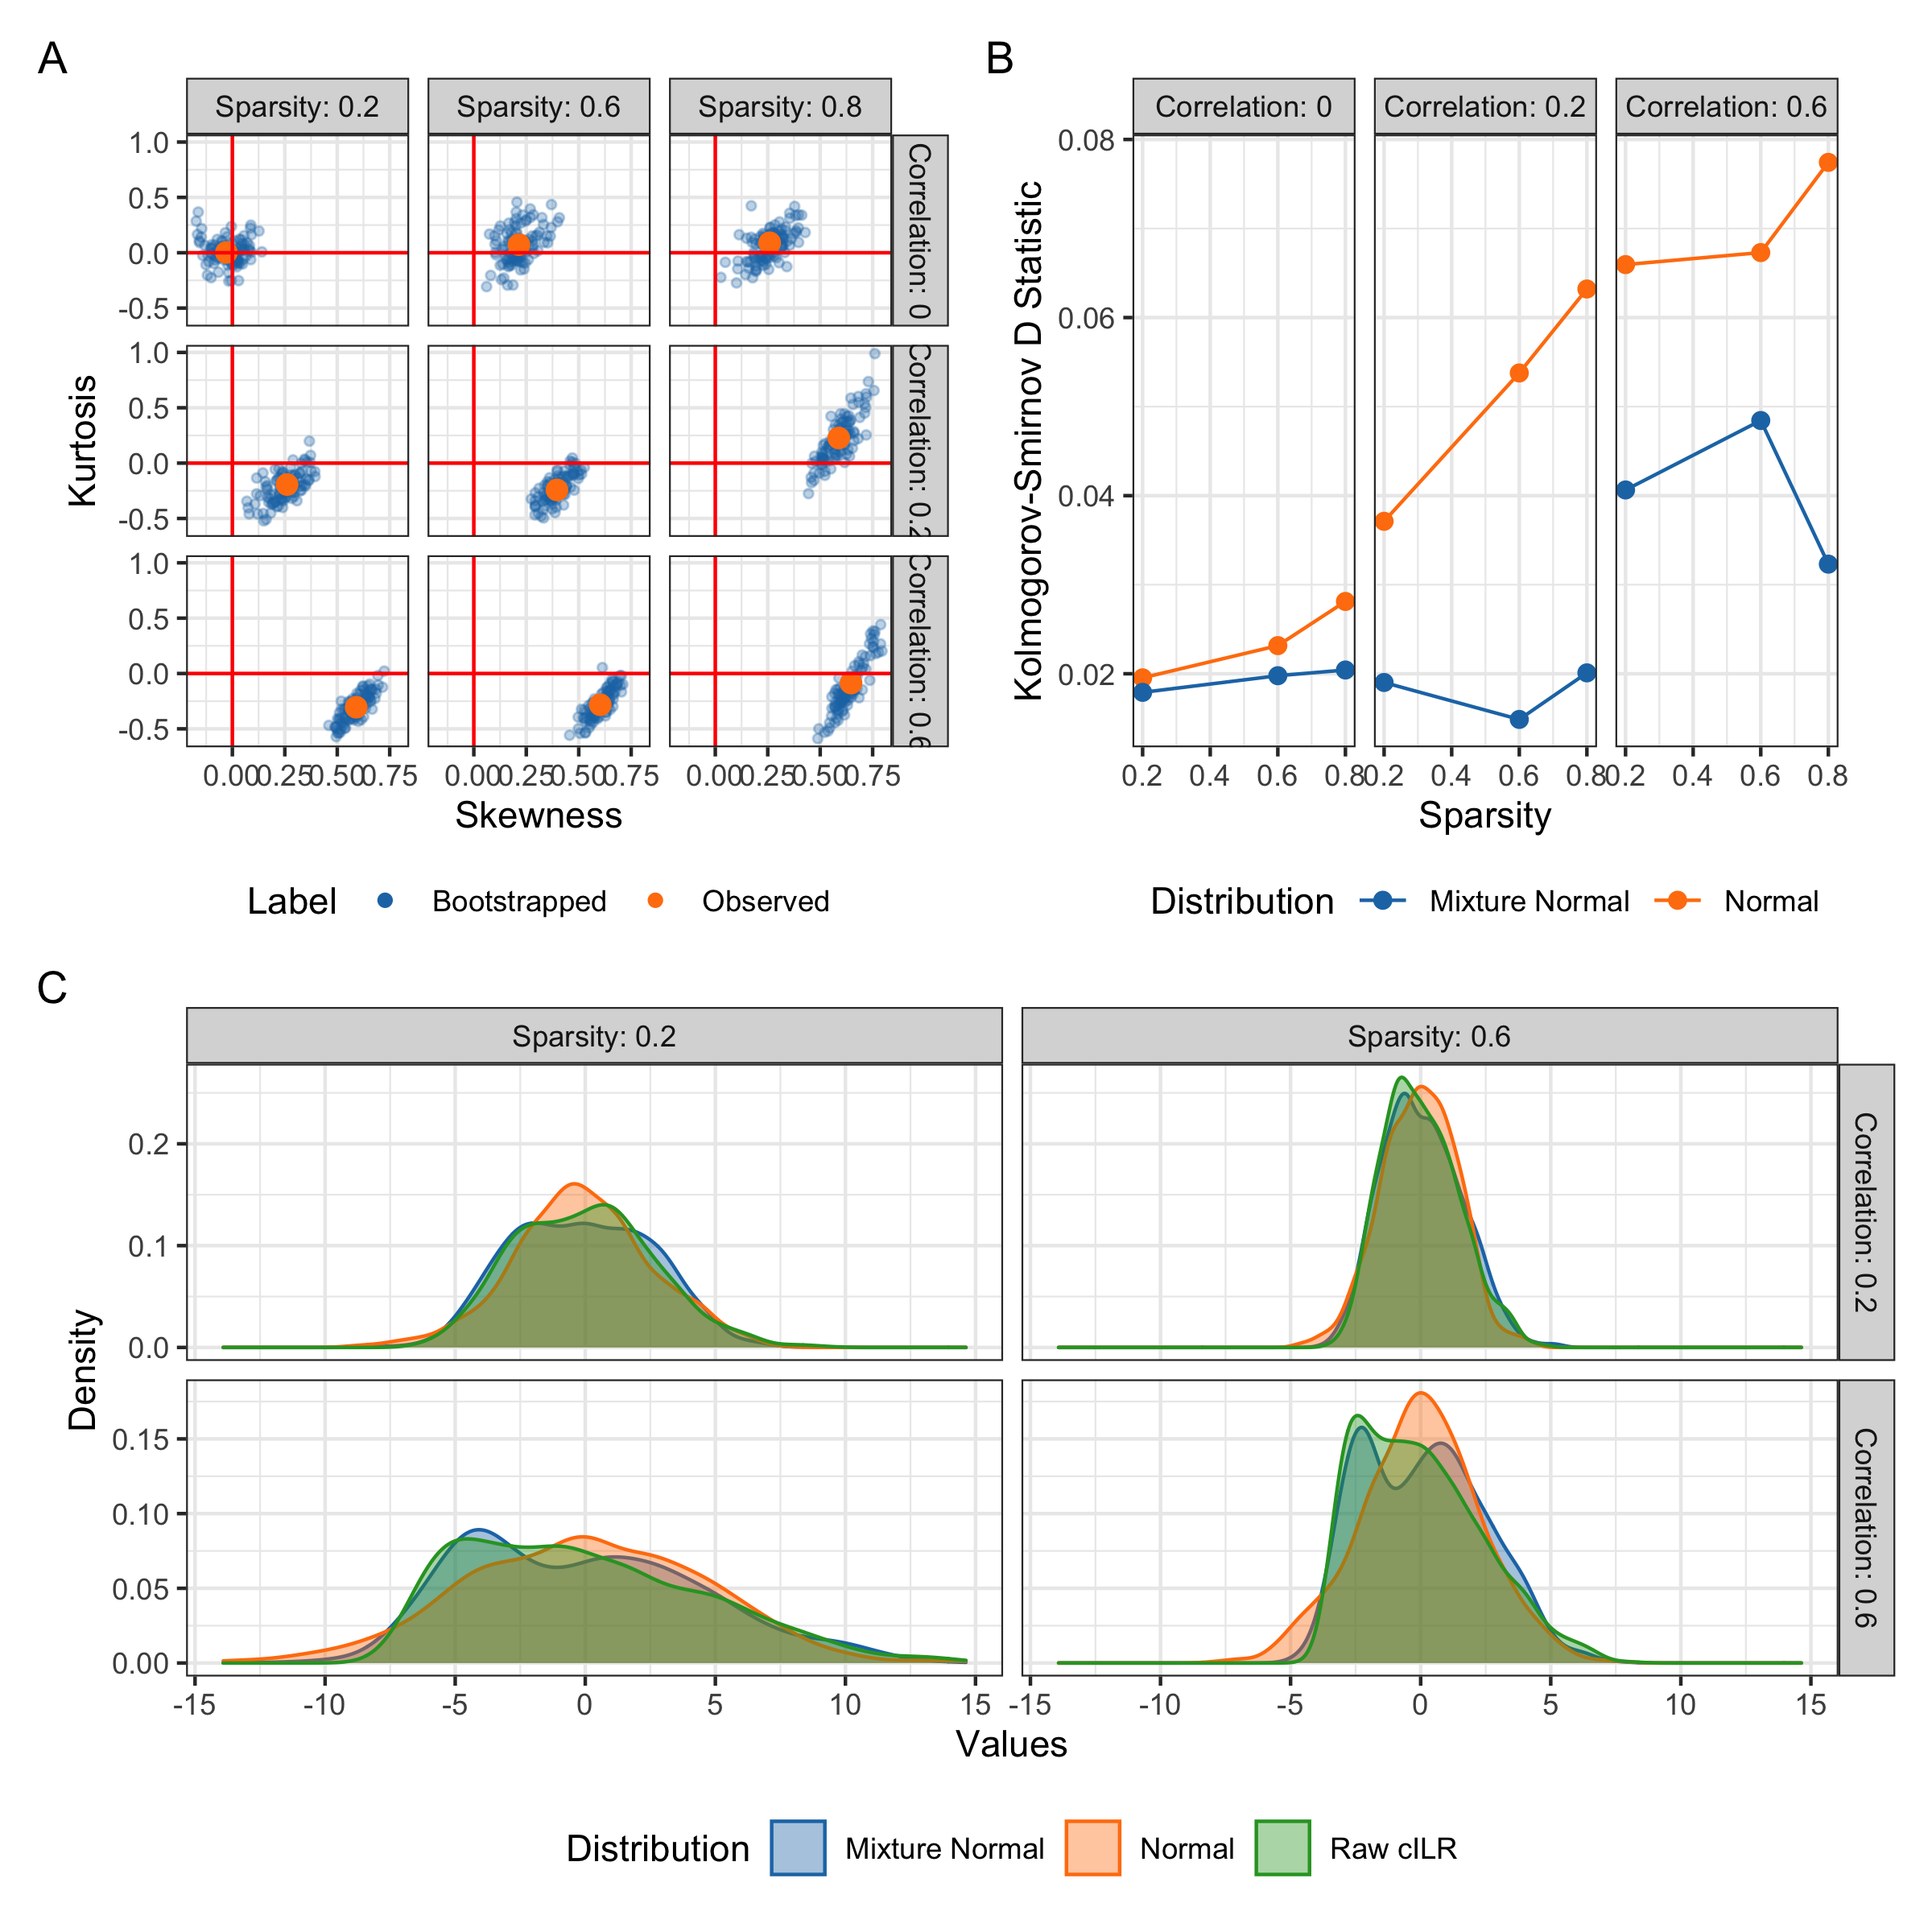
\includegraphics[width=\linewidth]{figures/kurtosis_skewness_gof.png}
    \caption{{\bf Properties of the null distribution of \DIFdelbeginFL \DIFdelFL{cILR }\DIFdelendFL \DIFaddbeginFL \DIFaddFL{CBEA }\DIFaddendFL under the global null simulations}. Panel \textbf{(B)} presents kurtosis and skewness of \DIFdelbeginFL \DIFdelFL{cILR }\DIFdelendFL \DIFaddbeginFL \DIFaddFL{CBEA }\DIFaddendFL scores while panel \textbf{(A)} presents the goodness of fit (as Kolmogorov-Smirnov D statistic) for mixture normal and normal distributions. Panel \textbf{(C)} is a density plot of the shape of the null distribution. Results indicated the necessity of estimating an empirical null and demonstrating that the mixture distribution was the better fit compared to the basic normal.}
    \label{fig:1}
\end{figure}

Additionally, the degree of kurtosis and skewness also suggests that the normal distribution itself might not be a good approximation of the null. To address this issue, we also evaluated a \DIFdelbegin \DIFdel{mixture distribution of two normal components}\DIFdelend \DIFaddbegin \DIFadd{two-component normal mixture distribution}\DIFaddend . Panel B of Fig~\ref{fig:1} demonstrates the goodness of fit of the mixture normal and the normal distribution using Kolmogorov-Smirnov (KS) test statistic computed on fitted normal and mixture normal distribution when fitted on \DIFdelbegin \DIFdel{cILR }\DIFdelend \DIFaddbegin \DIFadd{CBEA }\DIFaddend scores in simulation scenarios under the global null. We can see that the mixture normal distribution is a better fit (lower KS scores) than the normal distribution across both sparsity and correlation settings. 

We performed our empirical null estimation by fitting our distribution of choice and computing relevant parameters on raw \DIFdelbegin \DIFdel{cILR }\DIFdelend \DIFaddbegin \DIFadd{CBEA }\DIFaddend scores on taxa-permuted data (equivalent to gene permutation in the gene expression literature). As such, the null distribution is characterized by scores computed on sets of equal size with randomly drawn taxa. 
\DIFdelbegin \DIFdel{However, null distribution based on taxa-permutation is sensitive to inter-taxa correlations within the set \mbox{%DIFAUXCMD
\cite{wu2012}}\hspace{0pt}%DIFAUXCMD
. Since the permutation procedure does not preserve correlation structures, estimating parameters from empirical scores on permuted data will underestimate the variance inflation due to correlation. We account for this by combining the mean estimate from permuted data with }\DIFdelend \DIFaddbegin 

\subsubsection*{\DIFadd{Variance inflation due to inter-taxa correlation}}  
\DIFadd{When taxa within a set are highly correlated, }\DIFaddend the variance \DIFdelbegin \DIFdel{estimate from unpermuted data, where the inter-taxa correlation structure remains undisturbed. However, this procedure assumes that the variance of cILR is equal under both the null and alternate hypotheses. }%DIFDELCMD < 

%DIFDELCMD < %%%
\subsection*{\DIFdel{Evaluation}}
%DIFAUXCMD
\DIFdel{All code and data sets used for evaluation of this method is publicly available and can be found on GitHub (}\href{www.github.com/qpmnguyen/cILR\_analysis}{\DIFdel{qpmnguyen/cILR\_analysis}}%DIFAUXCMD
\DIFdel{) . 
}%DIFDELCMD < 

%DIFDELCMD < %%%
\subsubsection*{\DIFdel{Parametric Simulations}}  
%DIFAUXCMD
\DIFdel{To address the performance of cILR for different modeling tasks, we simulated microbiome count data under the assumption that it follows a zero-inflated negative binomial distribution, which is a good fit for real microbiome relative abundance data \mbox{%DIFAUXCMD
\cite{calgaro2020}}\hspace{0pt}%DIFAUXCMD
. Suppose $X_{ij}$ are observed counts for a sample }\DIFdelend \DIFaddbegin \DIFadd{of the sample mean of taxon-wise statistics is inflated. Without loss of generalizability, for a set of taxa with taxa-specific statistics $x_1, ..., x_p$ we have the variance of the mean $\bar{x}$ to be:  
}\begin{equation} \DIFadd{\label{vareq:1}
    Var(\bar{x}) = \frac{1}{m^2}\left(\sum_{i = 1}(\sigma_i^2) + \sum_{i < j}\rho_{ij}\sigma_i\sigma_j\right)
}\end{equation}
\DIFadd{where $\sigma_i$ is the standard deviation of taxon }\DIFaddend $i$ \DIFdelbegin \DIFdel{and taxon $j$, then we have the following probability model
}\begin{displaymath}
    \DIFdel{\mathbf{X}_{ij} =
      \begin{cases}
        0 & \text{with probability $p_j$}\\
        \mathbf{NB}(\mu_j, \phi_j) & \text{with probability $1 - p_j$}\\
      \end{cases}       
}\end{displaymath}%DIFAUXCMD
%DIFDELCMD < 

%DIFDELCMD < %%%
\DIFdel{where $\mu_j$ and $\phi_j$ are mean and dispersion parameters, respectively. To incorporate a flexible correlation structure into our simulation model, we utilized the NorTA (Normal to Anything) method \mbox{%DIFAUXCMD
\cite{cario1997}}\hspace{0pt}%DIFAUXCMD
. Given an $n$ by $p$ matrix of values $\mathbf{U}$ sampled from multivariate normal distribution with correlation matrix $\mathbf{\rho}$}\DIFdelend \DIFaddbegin \DIFadd{while $\rho_{ij}$ is the correlation between $i$ and $j$. The second term of (\ref{vareq:1}) is the correlation dependent variance component, which goes to 0 if there is no correlation. The CBEA statistic follows a similar pattern. Since the geometric mean of a set of variables is equivalent to the exponential of the arithmetic mean of their logarithms}\DIFaddend , we can \DIFdelbegin \DIFdel{generate target microbiome count vector $\mathbf{X_{.j}}$ for taxa $j$ following the marginal distribution $\mathbf{NB}$ characterized by the negative binomial cumulative distribution function $\mathbb{F_{\mathbf{NB}}}$:  
}\DIFdelend \DIFaddbegin \DIFadd{re-write CBEA score for a set $k$ with size $K$ as follows:  
}\DIFaddend \begin{equation}\DIFdelbegin \DIFdel{\mathbf{X}_{.j} }\DIFdelend \DIFaddbegin \label{vareq:2}
    \DIFadd{M_{i,k} }\DIFaddend = \DIFdelbegin \DIFdel{\mathbb{F_{\mathbf{NB}}}^{-1}(\Phi_{U_i})
}\DIFdelend \DIFaddbegin \DIFadd{\sqrt{\frac{K(p - K)}{K + (p - K)}} }\left( \overbar{\log{X_{i,j|j \in K}}} \DIFadd{- }\overbar{\log{X_{i,j|j \notin K}}} \right)   
\DIFaddend \end{equation}
\DIFdelbegin \DIFdel{In this instance, for each taxon }\DIFdelend \DIFaddbegin \DIFadd{where $p$ is the overall number of taxa, }\DIFaddend $j$ \DIFdelbegin \DIFdel{, we set elements in $\mathbf{U}_{.j}$ to be zero with probability $p_j$ and applied $\mathbf{NB}^{-1}(\mu_j, \phi_j)$ on non-zero elements to generate our final count matrix $\mathbf{X}$. To ensure that our simulations match closely to real data, we fitted negative binomial distribution using a maximum likelihood approach (with the }\emph{\DIFdel{fitdistrplus}} %DIFAUXCMD
\DIFdel{package in R \mbox{%DIFAUXCMD
\cite{delignette-muller2015}}\hspace{0pt}%DIFAUXCMD
) to non-zero counts for each taxon from 16S rRNA profiling of stool samples from the Human Microbiome Project (HMP). We take the median values of the estimated mean and dispersion parameters as the baseline of our simulations. For simplicity, we assumed that inter-taxa correlation follows an exchangeable structure
}%DIFDELCMD < 

%DIFDELCMD < \noindent %%%
\textbf{\DIFdel{Single Sample Enrichment}}%DIFAUXCMD
\DIFdel{: To assess }\DIFdelend \DIFaddbegin \DIFadd{is the index of a taxa and $K$ is the set of indices of taxa in set $k$. The CBEA statistic then looks similar to a t-statistic for difference in means of log-transformed proportions. As such, the pooled variance of CBEA is dependent on the variance inflation of both mean components $\overbar{\log{X_{i,j|j \in K}}}$ and $\overbar{\log{X_{i,j|j \notin K}}}$. The result of this variance inflation is inflated }\DIFaddend type I error \DIFdelbegin \DIFdel{rate and power for enrichment significance testing at the sample level, we simulated data based on the schema above, and assessed enrichment for one focal set. Type I error was obtained under the global null as the number of samples where the null hypothesis was rejected at $\alpha = 0.05$ over the total number of samples (which represents the total number of hypotheses tested). Power was obtained using the same formulation as type I error rate but under the global alternate. We treated type I error and power as estimates of binomial proportions and utilized the Agresti-Couli \mbox{%DIFAUXCMD
\cite{agresti1998} }\hspace{0pt}%DIFAUXCMD
formulation to calculate 95\% confidence intervals. Across both analyses, we varied sparsity levels ($p = 0.2, 0.4, 0.6$) and }\DIFdelend \DIFaddbegin \DIFadd{since highly correlated sets are also detected as significantly enriched. 
}

\DIFadd{However, as Wu et al. \mbox{%DIFAUXCMD
\cite{wu2012} }\hspace{0pt}%DIFAUXCMD
showed, performing column permutation to estimate the null distribution of a competitive test statistic doesn't allow for adequate capture of this variance inflation factor since the permutation procedure disrupts the natural correlation structure of the original variables. It is important to address this problem since there is strong }\DIFaddend inter-taxa correlation within the \DIFdelbegin \DIFdel{set ($\rho = 0, 0.2, 0.5$) . For type I error analysis, we also varied the size of the set (50, 100, 150) . For power analyses, set size was kept constant at 100 but different effect sizes (fold change of 1.5, 2, and 3). All sample sizes were set at 10,000. 
}%DIFDELCMD < 

%DIFDELCMD < %%%
\DIFdel{For classifiability, we evaluated the scores against the true labels per sample (indicating the sample has a set with inflated counts) using the area under the receiving operator curve (AUROC/AUC). This is a strategy used in Frost \mbox{%DIFAUXCMD
\cite{frost2020a} }\hspace{0pt}%DIFAUXCMD
which evaluates the informativeness of scores by assessing the relative ranking of samples (i. e. whether samples with inflated counts are highly ranked using estimated scores).  DeLong 95\% confidence intervals for AUC \mbox{%DIFAUXCMD
\cite{delong1988} }\hspace{0pt}%DIFAUXCMD
were obtained for each estimate. Simulation settings for classification performance were identical to power analyses as detailed in the previous paragraph}\DIFdelend \DIFaddbegin \DIFadd{microbiome \mbox{%DIFAUXCMD
\cite{kurtz2015a}}\hspace{0pt}%DIFAUXCMD
. Our strategy for addressing issue is location (or mean) estimate from the column permuted raw score matrix with the spread (or variance) estimate from the original un-permuted scores. This still allows us to leverage the null generated via column permutation while using the proper variance estimate taken from scores where the correlation structure has not been disrupted. As such, this procedure assumes that the variance of the test statistic under the alternate hypothesis is the same as that of the null. Details of the computational implementation to this estimation process can be found in the Supplementary Materials}\DIFaddend .   

\DIFdelbegin %DIFDELCMD < \noindent %%%
\textbf{\DIFdel{Differential Abundance Analysis}}%DIFAUXCMD
\DIFdel{: To assess type I error rate and power for differential abundance testing task, we simulated data based on the schema above, and assessed differential abundance of 50 sets with 100 taxa per set across 20 replicates per simulation condition. Type I error is calculated as the number of differentially abundant sets over the total number of sets for each simulation under the global null. Power is defined similarly, but instead under the global alternate hypothesis. Estimates and confidence intervals for type I error and power are calculated as cross-replicate mean and standard error. A set is differentially abundant when all taxa within a set are differentially abundant with the same effect size. Across both analyses, we varied sparsity levels ($p = 0.2, 0.4, 0.6$), and inter-taxa correlation within the set ($\rho = 0, 0.2, 0.5$). Half of the sets are differentially abundant across case/control status with varying effect sizes (fold change of 1.5, 2, and 3). Due to the compositional nature of microbiome taxonomic data, simple inflation of raw counts would cause an artificial decrease in the abundance of the remaining un-inflated sets . As such, we applied a compensation procedure as described in Hawinkel et al. \mbox{%DIFAUXCMD
\cite{hawinkel2019} }\hspace{0pt}%DIFAUXCMD
to ensure the validity of simulation results. All sample sizes were set at 2,000.    
}\DIFdelend \DIFaddbegin \DIFadd{However, set-based analysis is an exploratory approach that can help generate functionally informative hypotheses, and as such users might not want strict type I error control in favor of higher power. This is especially true for competitive hypotheses, where its stricter formulation compared to the self-contained approach implies that the test naturally has lower power \mbox{%DIFAUXCMD
\cite{goeman2007, ackerman2009}}\hspace{0pt}%DIFAUXCMD
. Furthermore, sets that are highly correlated compared to background can be biologically relevant. Therefore, CBEA provides an option for users to specify whether correlation adjustment is desired. 
}\DIFaddend 

\DIFdelbegin %DIFDELCMD < \noindent %%%
\textbf{\DIFdel{Prediction}}%DIFAUXCMD
\DIFdel{: To assess predictive performance, we generated predictors based on the simulation schema presented above and evaluated prediction for both binary and continuous outcomes using a standard random forest model \mbox{%DIFAUXCMD
\cite{breiman2001}}\hspace{0pt}%DIFAUXCMD
. For binary outcomes, we use AUC similar to the classification analyses above. For continuous outcomes, we used root mean squared error (RMSE). All predictive model fitting was performed using }\emph{\DIFdel{tidymodels}} %DIFAUXCMD
\DIFdel{\mbox{%DIFAUXCMD
\cite{kuhn2020} }\hspace{0pt}%DIFAUXCMD
suite of packages.  Across both learning tasks, we varied sparsity ($p = 0.2, 0.4, 0.6$), and inter-taxa correlation ($\rho = 0, 0.2, 0.5$).  
Continuous outcomes $Y_{cont}$ were generated as linear combinations of taxa counts. }\begin{displaymath}
    \DIFdel{Y_{cont} = f(\mathbf{X}) + \mathbf{\epsilon}
}\end{displaymath}%DIFAUXCMD
\DIFdel{where $\mathbf{\epsilon} \sim N(0, \sigma_{\epsilon}^2)$ and $f(\mathbf{X}) = \beta_0 + \mathbf{X}\mathbf{\beta}$. For each simulation, we set $\beta_0$ to be $\frac{6}{\sqrt{10}}$ similar to \mbox{%DIFAUXCMD
\cite{xiao2018}}\hspace{0pt}%DIFAUXCMD
. The degree of model saturation (the number of non zero $\mathbf{\beta}$ values) were varied between 0.1 and 0.5, and signal to noise ratio (SNR = $\frac{\sigma(f(\mathbf{X}))}{\sigma_{\epsilon}}$)was varied between 1.5, 2, and 3. 
}%DIFDELCMD < 

%DIFDELCMD < %%%
\DIFdel{For binary outcomes, we generate $Y_{binary}$ as Bernoulli draws with probability $p_{binary}$, where 
}\begin{displaymath}
    \DIFdel{p_{binary} = \frac{1}{1 + \exp(f(\mathbf{X}) + \mathbf{\epsilon})}
}\end{displaymath}%DIFAUXCMD
\DIFdel{To ensure a balance of classes, we applied the strategy described in Dong et al. \mbox{%DIFAUXCMD
\cite{dong2020} }\hspace{0pt}%DIFAUXCMD
where the associated $\beta$ values are evenly split between positive and negative associations. All data sets generated from prediction tasks have 2,000 samples with 5,000 taxa over 50 sets with a size of 100 taxa per set. }%DIFDELCMD < 

%DIFDELCMD < %%%
\subsubsection*{\DIFdel{Real Datasets}}
%DIFAUXCMD
%DIFDELCMD < 

%DIFDELCMD < %%%
\DIFdel{In additionto simulation analyses, we also evaluated our method using real data sets based on both 16S rRNA gene sequencing and whole-genome sequencing. All data sets are obtained from either the }\DIFdelend \DIFaddbegin \section*{\DIFadd{Evaluation}} \label{evaluation}
\DIFadd{We based our evaluation strategy on gene set testing benchmarking standards set by Geistlinger et al. \mbox{%DIFAUXCMD
\cite{geistlinger2021} }\hspace{0pt}%DIFAUXCMD
and utilized the same approaches whenever possible. All data sets are obtained from either the }\DIFaddend \emph{curatedMetagenomicData} \cite{pasolli2017} and \emph{HMP16SData} \cite{schiffer2019} R packages (2020-10-02 \DIFdelbegin \DIFdel{snapshot), or downloaded from the Qiita platform \mbox{%DIFAUXCMD
\cite{gonzalez2018}}\hspace{0pt}%DIFAUXCMD
.  
}\DIFdelend \DIFaddbegin \DIFadd{snapshot), or downloaded from the Qiita platform \mbox{%DIFAUXCMD
\cite{gonzalez2018}}\hspace{0pt}%DIFAUXCMD
. All code and data sets used for evaluation of this method is publicly available and can be found on GitHub (}\href{www.github.com/qpmnguyen/CBEA\_analysis}{\DIFadd{qpmnguyen/CBEA\_analysis}}\DIFadd{). Additional packages used to support this analysis includes: }\emph{\DIFadd{tidyverse}} \DIFadd{\mbox{%DIFAUXCMD
\cite{wickham2019}}\hspace{0pt}%DIFAUXCMD
, }\emph{\DIFadd{pROC}} \DIFadd{\mbox{%DIFAUXCMD
\cite{robin2011}}\hspace{0pt}%DIFAUXCMD
, }\emph{\DIFadd{phyloseq}} \DIFadd{\mbox{%DIFAUXCMD
\cite{mcmurdie2014}}\hspace{0pt}%DIFAUXCMD
, }\emph{\DIFadd{mia}} \DIFadd{\mbox{%DIFAUXCMD
\cite{ernst2021}}\hspace{0pt}%DIFAUXCMD
, }\emph{\DIFadd{targets}} \DIFadd{\mbox{%DIFAUXCMD
\cite{landau2021}}\hspace{0pt}%DIFAUXCMD
.   
}\DIFaddend 

\DIFdelbegin %DIFDELCMD < \noindent %%%
\textbf{\DIFdel{Single Sample Enrichment}}%DIFAUXCMD
\DIFdel{: To assess the false discovery rate and true discovery rate of cILR in sample-level enrichment testing, we utilized the }\DIFdelend \DIFaddbegin \subsection*{\DIFadd{Statistical significance}}
\DIFadd{We evaluate the inference procedure of CBEA compared to alternate methods using two approaches: randomly sampled taxa sets and sample label permutation. These analyses were performed on the }\DIFaddend 16S \DIFdelbegin \DIFdel{rRNA gene sequencing of the oral microbiome at the gingival subsite from the Human Microbiome Project \mbox{%DIFAUXCMD
\cite{consortium2012, proctor2019}}\hspace{0pt}%DIFAUXCMD
. We utilized this data set following the approach outlined in Calagaro et al. \mbox{%DIFAUXCMD
\cite{calgaro2020}}\hspace{0pt}%DIFAUXCMD
. }\DIFdelend \DIFaddbegin \DIFadd{rRNA gene sequencing of the oral microbiome from the Human Microbiome Project \mbox{%DIFAUXCMD
\cite{consortium2012, proctor2019}}\hspace{0pt}%DIFAUXCMD
. This data set contains 369 samples split into two subsites: supragingival and subgingival. We processed this data set by removing all samples with total read counts less than 1000 and OTUs whose presence (at least 1 count) is in 10\% of samples or less.  
}

\subsubsection*{\DIFadd{Sample-level inference}} 
\DIFadd{Due to CBEA's self-contained null hypothesis, we can perform inference at the sample level for the enrichment of a set. We evaluated this application by generating one random taxa of different sizes $S \in \{20, 50, 100, 150, 200\}$ across 500 iterations. Random sets can act as our estimate for type I error since this matches the CBEA null hypothesis stated in }\nameref{methods}\DIFadd{, where we expect within each sample sets of randomly drawn taxa should not be significantly enriched compared to the remainder background taxa. For this evaluation, we estimated type I error as the fraction of samples that detects our random set as significant at a p-value threshold of 0.05 with confidence bands computed from the standard error across all iterations.  Additionally, this analysis also demonstrate whether CBEA is sensitive to different set sizes.  
}

\subsubsection*{\DIFadd{Population-level inference}} 
\DIFadd{We can perform enrichment testing at the population level by generating corresponding sample level CBEA scores and performing a two-sample test such as Welch's t-test. In order to evaluate CBEA under this context, we generated CBEA scores of sets representing genus-level annotation in above gingival data set \mbox{%DIFAUXCMD
\cite{consortium2012, proctor2019} }\hspace{0pt}%DIFAUXCMD
and applied a t-test to test for enrichment (similar to GSVA \mbox{%DIFAUXCMD
\cite{hanzelmann2013}}\hspace{0pt}%DIFAUXCMD
) across a randomly generated variable indicating case/control status (repeated 500 times). Type I error is estimated as the fraction of sets per iteration found to be significantly enriched with confidence bands computed from the standard error across all iterations. In addition, we also performed a random set analysis assessment, where we generated 100 sets of different set sizes $S \in \{20, 50, 100, 150, 200\}$ and evaluated the fraction of genera that were found to be differentially abundant across the original labels (supragingival versus subgingival subsite). 95\% confidence intervals were computed using the Agresti-Couli approach \mbox{%DIFAUXCMD
\cite{agresti1998}}\hspace{0pt}%DIFAUXCMD
.  
}

\subsection*{\DIFadd{Phenotype relevance}}
\DIFadd{We want to evaluate whether sets found to be significantly enriched by CBEA are relevant to the research question. To perform this assessment, we relied on the gingival data set mentioned prior \mbox{%DIFAUXCMD
\cite{consortium2012, proctor2019}}\hspace{0pt}%DIFAUXCMD
. }\DIFaddend This data set \DIFdelbegin \DIFdel{is approximately labeled, where aerobic microbes are }\DIFdelend \DIFaddbegin \DIFadd{was chosen due to its clear biological interpretation that can serve as the ground truth. Specifically, we expect aerobic microbes to be }\DIFaddend enriched in the supragingival subsite where the biofilm is exposed to the open air, while conversely anaerobic microbes thrive in the subgingival site \cite{thurnheer2016}. \DIFdelbegin \DIFdel{Here, we assessed the enrichment of aerobic microbes across all samples, we considered the false positive rate as the number of samples from the subgingival site with significant enrichment, and the true positive rate as the number of supragingival samples with significant enrichment. Microbial tropism annotation at the genus level was from }\DIFdelend \DIFaddbegin \DIFadd{Genus-level annotations for microbial metabolism from }\DIFaddend Beghini et al. \cite{beghini2019} and was \DIFdelbegin \DIFdel{downloaded directly }\DIFdelend \DIFaddbegin \DIFadd{obtained }\DIFaddend from the GitHub repository associated with Calagaro et al. \cite{matteocalgaro2020}. \DIFdelbegin %DIFDELCMD < 

%DIFDELCMD < \noindent %%%
\textbf{\DIFdel{Differential Abundance Analsysis}}%DIFAUXCMD
\DIFdel{: To assess type I error using cILR scores in differential abundance analysis, we utilized the 16S rRNA gene sequencing of stool samples from the Human Microbiome Project \mbox{%DIFAUXCMD
\cite{consortium2012, proctor2019}}\hspace{0pt}%DIFAUXCMD
. Here, we randomly assign samples a label of case or control, and repeated this process 500 times, assessing all candidate methods at each iteration. Type I error is then the number of taxa identified as differentially abundant across all tested taxa.  
For the true positive rate, we used the same gingival data set as described above. However, instead of testing for aerobic microbes as a group, the true positive rate is }\DIFdelend \DIFaddbegin \DIFadd{For sample-level inference, we assessed power as the fraction of supragingival samples where aerobic microbes are significantly enriched. For population-level inference, power is }\DIFaddend the \DIFdelbegin \DIFdel{number of aerobic}\DIFdelend \DIFaddbegin \DIFadd{fraction of sets representing genus level taxonomic assignments that were significant across subsite labels.  
}

\DIFadd{In addition to statistical power, we also assessed phenotype relevance through evaluating whether highly ranked sets based on CBEA scores are more likely to be enriched according to ground truth. This is represented by the area under the receiving operator curve (AUROC}\DIFaddend /\DIFdelbegin \DIFdel{anaerobic genera identified as differentially abundant across all aerobic or anaerobic genera. }\DIFdelend \DIFaddbegin \DIFadd{AUC) scores computed on CBEA scores against true labels (similar approach was used to evaluate VAM \mbox{%DIFAUXCMD
\cite{frost2020}}\hspace{0pt}%DIFAUXCMD
). DeLong 95\% confidence intervals for AUROC \mbox{%DIFAUXCMD
\cite{delong1988} }\hspace{0pt}%DIFAUXCMD
were obtained for each estimate. 
}\DIFaddend 

\DIFdelbegin %DIFDELCMD < \noindent %%%
\textbf{\DIFdel{Disease Prediction}}%DIFAUXCMD
\DIFdel{: To assess predictive power, we utilized the whole }\DIFdelend \DIFaddbegin \subsection*{\DIFadd{Disease Prediction}}
\DIFadd{CBEA scores can also be used downstream analyses such as disease prediction tasks. We utilized two data sets for this evaluation: 
}

\begin{enumerate}
\item \DIFadd{Whole }\DIFaddend genome sequencing of stool samples \DIFdelbegin \DIFdel{of }\DIFdelend \DIFaddbegin \DIFadd{from }\DIFaddend inflammatory bowel disease (IBD) patients \DIFdelbegin \DIFdel{from }\DIFdelend \DIFaddbegin \DIFadd{in }\DIFaddend the MetaHIT consortium \cite{nielsen2014}. This data set contains 396 samples from a cohort of European adults, where 195 adults were classified as having IBD (which includes patients diagnosed with either ulcerative colitis or Crohn's disease). \DIFdelbegin \DIFdel{Additionally,we also utilized a similar data set from Gevers et al. \mbox{%DIFAUXCMD
\cite{gevers2014} }\hspace{0pt}%DIFAUXCMD
which also profiles the gut microbiome of IBD patients and controls but using }\DIFdelend \DIFaddbegin \DIFadd{We processed this data by removing all samples with less than 1,000 total read counts as well as any OTU who was present (with non-zero proportions) in 10\% of samples or less. Prior to model fitting, we back-transformed relative abundances into count data (to align the format with our }\DIFaddend 16S \DIFaddbegin \DIFadd{rRNA gene sequencing data set) using provided total number of reads aligned to MetaPhlan marker genes (per sample).   
}

\item \DIFadd{16S }\DIFaddend rRNA gene sequencing \DIFaddbegin \DIFadd{of stool samples from IBD patients in the pediatric RISK cohort \mbox{%DIFAUXCMD
\cite{gevers2014}}\hspace{0pt}%DIFAUXCMD
}\DIFaddend . This data set contains 16S rRNA gene sequencing samples from a cohort of pediatric patients (ages $<$ 17) from the RISK cohort enrolled in the United States and Canada. Of the 671 samples obtained, 500 samples belong to patients with IBD. \DIFaddbegin \DIFadd{We processed this data set by removing all samples with less than 1,000 total read counts as well as any OTU who was present (at least 1 count) in 10\% of samples or less.   
}\end{enumerate}

\DIFadd{We evaluate disease prediction performance by fitting a random forest model \mbox{%DIFAUXCMD
\cite{breiman2001} }\hspace{0pt}%DIFAUXCMD
using inputs as CBEA scores to classify samples of patients with IBD and healthy controls. Random forest was chosen as a baseline learner due to its flexibility as an out-of-the-box model that is easy to fit. In this instance we evaluated predictive performance of a default random forest model (without hyperparameter tuning) AUROC after 10-fold cross validation. Additionally, we utilized SMOTE to correct for class imbalances \mbox{%DIFAUXCMD
\cite{chawla2002}}\hspace{0pt}%DIFAUXCMD
. Implementation was done using the }\emph{\DIFadd{tidymodels}} \DIFadd{suite of packages \mbox{%DIFAUXCMD
\cite{kuhn2020}}\hspace{0pt}%DIFAUXCMD
.   
}\DIFaddend 

\DIFdelbegin \subsubsection*{\DIFdel{Comparison Methods}}
%DIFAUXCMD
%DIFDELCMD < 

%DIFDELCMD < \noindent %%%
\textbf{\DIFdel{Single sample enrichment}}%DIFAUXCMD
\DIFdel{: For type I error and power analyses, we compared the cILR method with a naive Wilcoxon rank sum test.   
We added a pseudocount of 1 to all values. This is }\DIFdelend \DIFaddbegin \subsection*{\DIFadd{Comparison Methods}} 
\DIFadd{We benchmarked the statistical properties of CBEA against existing baseline approaches. For sample-level inference analyses, utilized the Wilcoxon rank-sum test, which non-parametrically tests the difference in mean counts between taxa from }\DIFaddend a \DIFdelbegin \DIFdel{non-parametric difference in means test, where we compared the abundance of taxa of a }\DIFdelend pre-defined set and its \DIFdelbegin \DIFdel{complement within a single sample. For classification performance}\DIFdelend \DIFaddbegin \DIFadd{remainder similar to CBEA. For assessments at the population level}\DIFaddend , we compared \DIFdelbegin \DIFdel{cILR methods against GSVA \mbox{%DIFAUXCMD
\cite{hanzelmann2013}}\hspace{0pt}%DIFAUXCMD
, ssGSEA \mbox{%DIFAUXCMD
\cite{barbie2009}}\hspace{0pt}%DIFAUXCMD
, and the W-statistic from the Wilcoxon rank sum test . All three approaches were applied directly on count data (after pseudocount). For GSVA, the Poisson kernel was used. 
}%DIFDELCMD < 

%DIFDELCMD < \noindent %%%
\textbf{\DIFdel{Differential Abundance}}%DIFAUXCMD
\DIFdel{: Since cILR are sample-level enrichment scores, we performed differential abundance by using a Wilcoxon Rank Sum test and Welch's t-test across case/control status on cILR generated scores. We added a pseudocount of 1 to all values. For comparison, we chose representative state-of-the-art methods in differential abundance analysis, namely }\DIFdelend \DIFaddbegin \DIFadd{CBEA against performing a standard test for differential abundance with set-level features generated via element-wise summations instead. We chose }\DIFaddend DESeq2 \DIFdelbegin \DIFdel{\mbox{%DIFAUXCMD
\cite{love2014,mcmurdie2014} }\hspace{0pt}%DIFAUXCMD
}\DIFdelend \DIFaddbegin \DIFadd{\mbox{%DIFAUXCMD
\cite{love2014} }\hspace{0pt}%DIFAUXCMD
}\DIFaddend and corncob \cite{martin2020} \DIFdelbegin \DIFdel{. For DESeq2, we performed a likelihood ratio test against an intercept only reduced model with dispersion estimated with local fit. For corncob, we also performed a likelihood ratio test against an intercept only reduced model without bootstrapping. 
}\DIFdelend \DIFaddbegin \DIFadd{because they represent both methods extrapolated from RNA-seq \mbox{%DIFAUXCMD
\cite{mcmurdie2014} }\hspace{0pt}%DIFAUXCMD
and those developed specifically for microbiome data.   
}\DIFaddend 

\DIFdelbegin %DIFDELCMD < \noindent %%%
\textbf{\DIFdel{Disease Prediction}}%DIFAUXCMD
\DIFdel{: We fit random forest on cILR scores, as well as ssGSEA \mbox{%DIFAUXCMD
\cite{hanzelmann2013} }\hspace{0pt}%DIFAUXCMD
and GSVA \mbox{%DIFAUXCMD
\cite{barbie2009} }\hspace{0pt}%DIFAUXCMD
similar to single sample enrichment section. We added a pseudocount of 1 to all values. Additionally, }\DIFdelend \DIFaddbegin \DIFadd{Since disease prediction models and rankings-based phenotype relevance analyses seek to evaluate the informativeness of CBEA scores instead of relying on computing p-values, we compared performance against other single sample based approaches from the gene set testing literature, specifically ssGSEA \mbox{%DIFAUXCMD
\cite{barbie2009} }\hspace{0pt}%DIFAUXCMD
and GSVA \mbox{%DIFAUXCMD
\cite{hanzelmann2013}}\hspace{0pt}%DIFAUXCMD
. Additionally, for evaluating prediction, }\DIFaddend we also compared performance \DIFdelbegin \DIFdel{using cILR }\DIFdelend against a standard analysis plan where \DIFaddbegin \DIFadd{inputs are count-aggregated sets with }\DIFaddend the centered log-ratio \DIFdelbegin \DIFdel{transformation }\DIFdelend (CLR) \DIFdelbegin \DIFdel{was applied to count-aggregated sets as inputs to a machine learning model}\DIFdelend \DIFaddbegin \DIFadd{transformation}\DIFaddend . 

\section*{Results}
In this section, we present \DIFdelbegin \DIFdel{the performance of our proposed method for three applicable microbiome analysis tasks: sample level enrichment, differential abundance, and disease prediction. We obtained these results from both parametric simulations and examples from real data}\DIFdelend \DIFaddbegin \DIFadd{results for evaluating statistical significance, phenotype relevance, and predictive performance. In addition to real data, we also evaluated models based on parametric simulations, where results can be found in the Supplemental Materials}\DIFaddend .   

\subsection*{\DIFdelbegin \DIFdel{Enrichment testing at the sample level}\DIFdelend \DIFaddbegin \DIFadd{Statistical Significance}\DIFaddend }
\DIFdelbegin \DIFdel{cILR }\DIFdelend \DIFaddbegin \subsubsection*{\DIFadd{Inference at the sample level}}
\DIFadd{CBEA }\DIFaddend provides significance testing \DIFdelbegin \DIFdel{for enrichment }\DIFdelend at the sample level \DIFdelbegin \DIFdel{using the null distribution estimation procedure described in }%DIFDELCMD < \nameref{methods}%%%
\DIFdel{. Here, we present empirical results for this application of cILR assessing type I error, power, and classification capacity}\DIFdelend \DIFaddbegin \DIFadd{through a self-contained competitive null hypothesis. Generating random sets approximate the global null setting where within each sample, sets generated by randomly sampling taxa should not be significantly more enriched than remainder taxa}\DIFaddend .   

\DIFdelbegin \subsubsection*{\DIFdel{Simulation studies}}
%DIFAUXCMD
\DIFdel{Panel A and B in }\DIFdelend \DIFaddbegin \begin{figure}[!h]
    \centering
    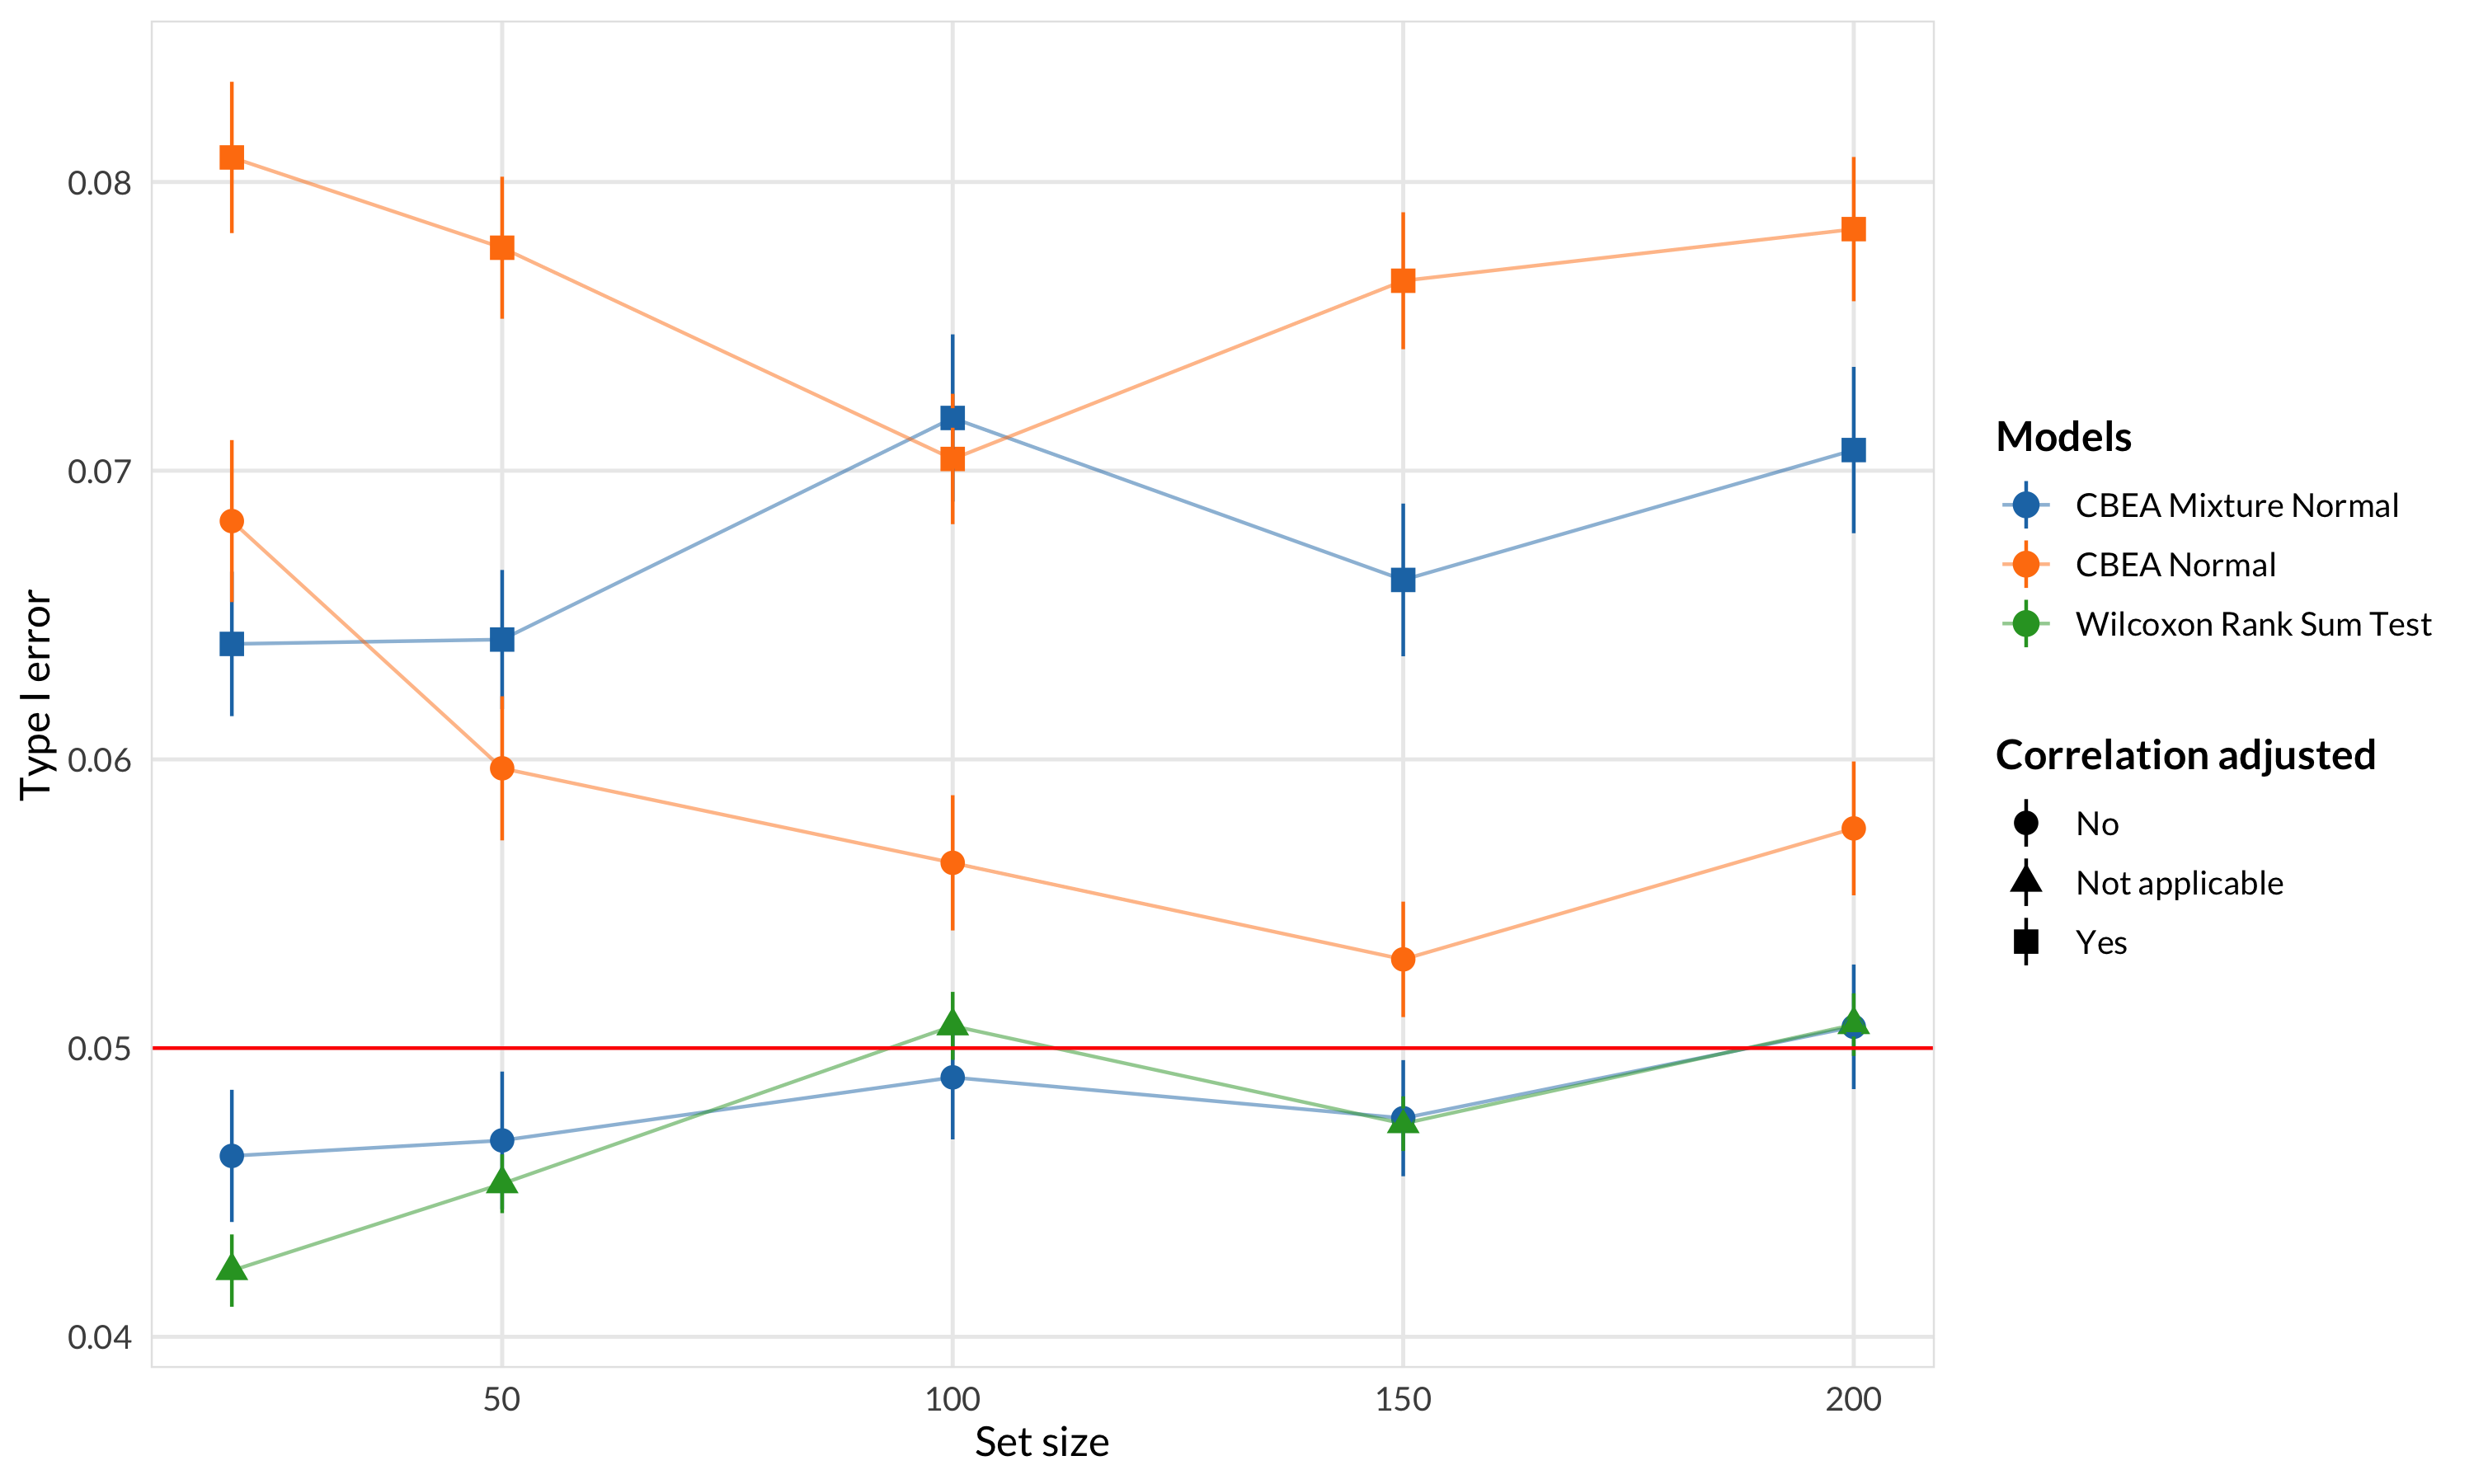
\includegraphics[width = \textwidth]{figures/data_ss_fdr_new.png}
    \caption{\DIFaddFL{Random taxa set analyses for inference at the sample level of CBEA under different parametric assumptions compared against a Wilcoxon rank-sum test. Type I error (}\emph{\DIFaddFL{y}}\DIFaddFL{-axis) was evaluated by generating random sets of different sizes (}\emph{\DIFaddFL{x}}\DIFaddFL{-axis) (500 replications per size) and computing the fraction of samples where the set was found to be significantly enriched at $\alpha = 0.05$. Error bars represent the mean type I error $\pm$ sample standard error computed across 500 replications of the experiment. Only the unadjusted CBEA with the mixture normal distribution and the Wilcoxon rank sum test were able to control for type I error at 0.05. All approaches are invariant to set sizes.}} 
    \label{fig:2}
\end{figure}

\DIFaddend Fig~\ref{fig:2} \DIFdelbegin \DIFdel{demonstrate }\DIFdelend \DIFaddbegin \DIFadd{demonstrates }\DIFaddend type I error \DIFdelbegin \DIFdel{and power respectively across different simulation conditions. We benchmarked the results of the cILR method against a naive }\DIFdelend \DIFaddbegin \DIFadd{of sample-level inference evaluated using the random set approach. The }\DIFaddend Wilcoxon rank sum test \DIFdelbegin \DIFdel{performed at the sample level, comparing the mean count difference between taxa in the set its complement. All methods demonstrate }\DIFdelend \DIFaddbegin \DIFadd{and unadjusted CBEA under mixture normal assumption demonstrated }\DIFaddend good type I error control at \DIFdelbegin \DIFdel{$\alpha = 0.05$ under zero correlation across all simulation conditions. However, under both medium ($\rho = 0.2$)and high ($\rho = 0.5$) correlation settings, both the Wilcoxon test and unadjusted cILR variants show high levels of }\DIFdelend \DIFaddbegin \DIFadd{the appropriate $\alpha$ level. This fits with our expectations since the mixture normal distribution has much better fit than the normal distribution especially at the tails (Fig~\ref{fig:1}). However, other variants of CBEA demonstrated }\DIFaddend inflated type I error, \DIFdelbegin \DIFdel{where Wilcoxon test performed the worst. On the other hand, adjusted cILR methods (under both distributions) control for }\DIFdelend \DIFaddbegin \DIFadd{especially correlation adjusted variants compared to their unadjusted counter parts. Encouragingly, all methods demonstrate consistent performance across all set sizes, with a slight increase in }\DIFaddend type I error at the \DIFdelbegin \DIFdel{appropriate $\alpha$ level even at high correlations}\DIFdelend \DIFaddbegin \DIFadd{highest levels}\DIFaddend .   

\DIFdelbegin %DIFDELCMD < \begin{figure}[!h]
%DIFDELCMD <     \centering
%DIFDELCMD <     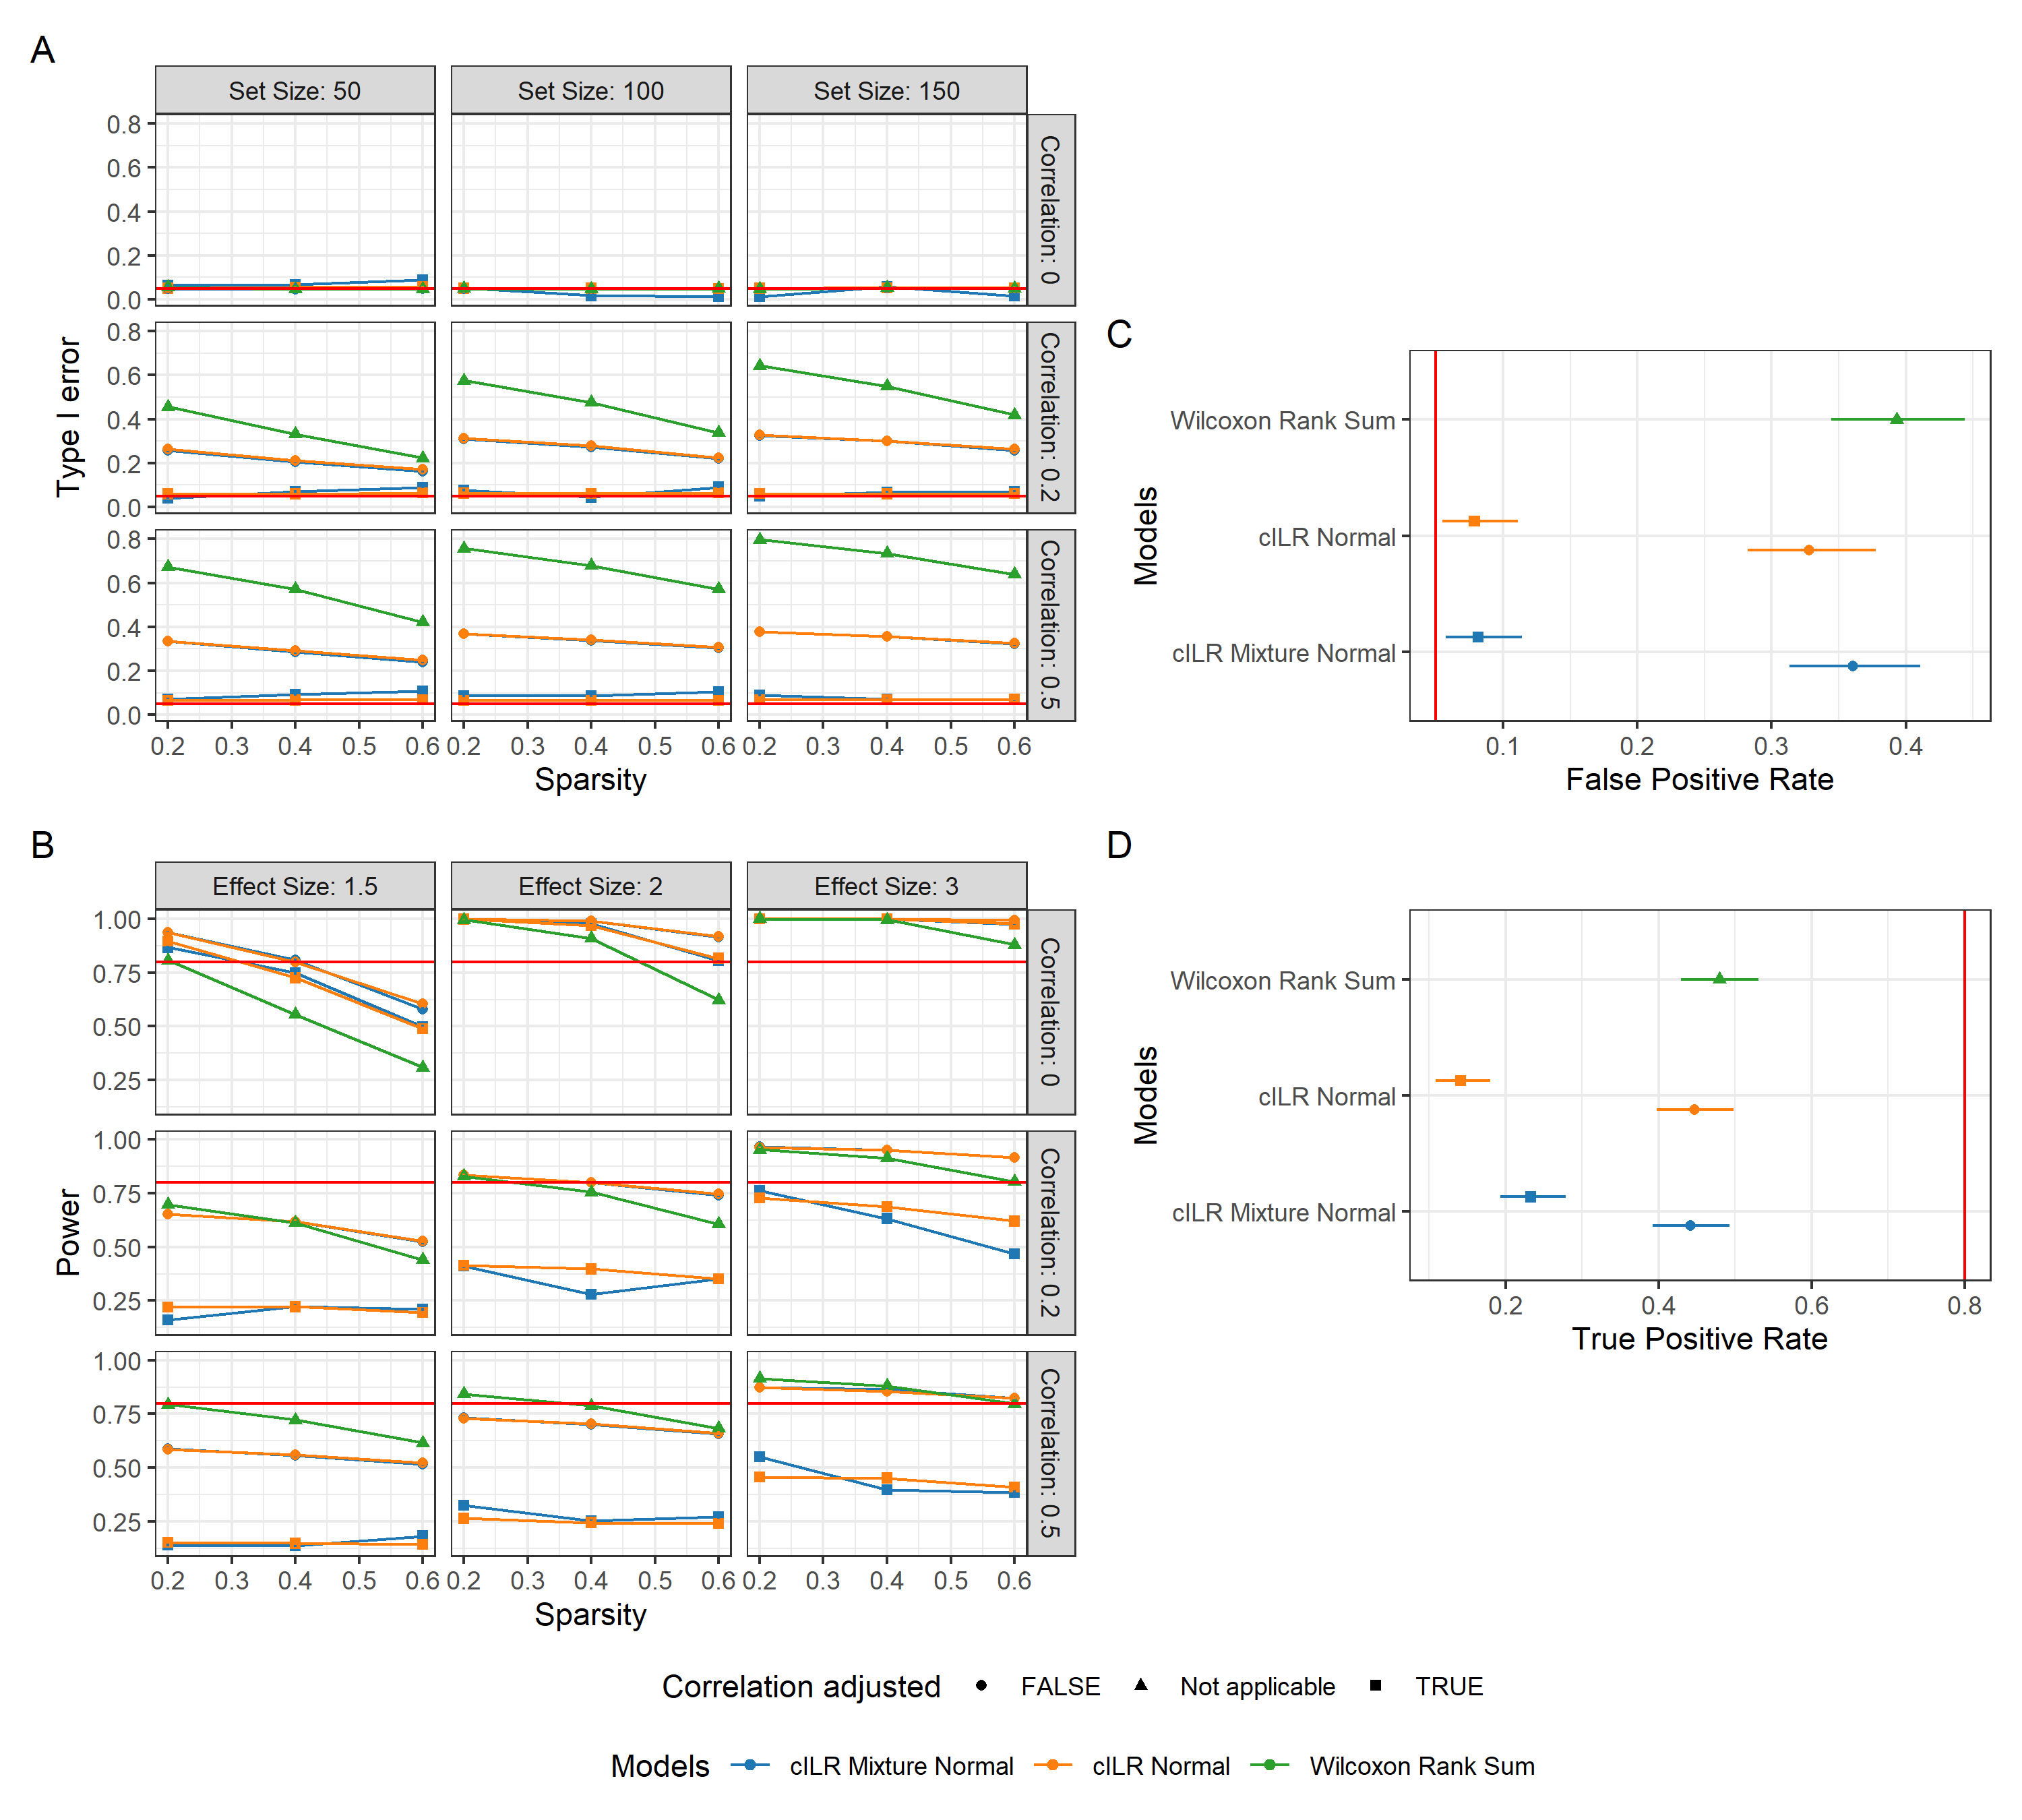
\includegraphics[width=\textwidth]{figures/sim_data_ss_hypo.png}
%DIFDELCMD <     %%%
%DIFDELCMD < \caption{%
{%DIFAUXCMD
\DIFdelFL{Sample-level inference with cILR under parametric simulations (}\textbf{\DIFdelFL{(A)}} %DIFAUXCMD
\DIFdelFL{and }\textbf{\DIFdelFL{B}}%DIFAUXCMD
\DIFdelFL{), and real data analysis (}\textbf{\DIFdelFL{(C)}} %DIFAUXCMD
\DIFdelFL{and }\textbf{\DIFdelFL{(D)}}%DIFAUXCMD
\DIFdelFL{). In simulation analyses, panel }\textbf{\DIFdelFL{(A)}} %DIFAUXCMD
\DIFdelFL{shows type I error rate, and panel }\textbf{\DIFdelFL{(B)}} %DIFAUXCMD
\DIFdelFL{shows power for single sample enrichment test for a specified set and was compared against a Wilcoxon rank sum test at $\alpha$ of 0.05. In real data analysis, panel }\textbf{\DIFdelFL{(C)}} %DIFAUXCMD
\DIFdelFL{shows the false-positive rate, and panel }\textbf{\DIFdelFL{(D)}} %DIFAUXCMD
\DIFdelFL{shows the true positive rate. For this analysis, 16S rRNA data from the oral microbiome of the gingival site was used. The set of aerobic microbes was tested for enrichment in all samples and was identified as correctly enriched if a significant $p$-value was obtained in supragingival samples. Confidence bounds were obtained using Agresti-Couli \mbox{%DIFAUXCMD
\cite{agresti1998} }\hspace{0pt}%DIFAUXCMD
approach. Adjusted cILR demonstrated control of type I error at the appropriate $\alpha$ level while remaining methods (not included in subsequent power analyses) showed an inflated type I error rate. However, this resulted in lower power for adjusted cILR methods.}}
    %DIFAUXCMD
%DIFDELCMD < \label{fig:2}
%DIFDELCMD < \end{figure}
%DIFDELCMD < 

%DIFDELCMD < %%%
\DIFdel{However, the trade-off for good }\DIFdelend \DIFaddbegin \DIFadd{Interestingly, simulation results (}\nameref{S1_Fig}\DIFadd{) showed an opposite pattern. Adjusted approaches were good at controlling for }\DIFaddend type I error\DIFdelbegin \DIFdel{control is demonstrably lower power, as shown in Fig~\ref{fig:2}B. In situations where there is no }\DIFdelend \DIFaddbegin \DIFadd{, especially under the low }\DIFaddend inter-taxa correlation \DIFdelbegin \DIFdel{, cILR still outperforms the wilcoxon rank sum test, however adjusted versions of cILR did not perform as well as un-adjusted ones. However, in higher correlation scenarios, the difference in power is much more dramatic. At the highest effect size (fold change of 3)and correlation ($\rho = 0.5$), adjusted cILR was only performing at 50\% power, while unadjusted cILR and wilcoxon }\DIFdelend \DIFaddbegin \DIFadd{values within the set (similar to generating random sets where the natural correlation structure is disrupted). In these simulations, unadjusted approaches and the Wilcoxon }\DIFaddend rank sum test \DIFdelbegin \DIFdel{were able to reach 80\%. These results indicate that both sparsity and inter-taxa correlation impacts power, with correlation having a much more dramatic impact especially for adjusted versions of cILR. Most importantly, cILR demonstrate higher power in all scenarios where }\DIFdelend \DIFaddbegin \DIFadd{had significant }\DIFaddend type I error \DIFdelbegin \DIFdel{is properly controlled.    
}\DIFdelend \DIFaddbegin \DIFadd{inflation with increasing correlation. All approaches seems to be invariant to the level of data sparsity.  
}\DIFaddend 

\DIFdelbegin \DIFdel{To further assess the utility of cILR in classifying samples with enriched sets, we generated AUC scores for different cILR scores using true labels of whether a sample has an inflated set. This analysis, therefore, assessed the relative ranking of samples using cILR scores whereby high scores should correspond to samples that are known to be inflated. Fig~\ref{fig:3} presents this result. We compared different variants of cILR against competing methods in the }\DIFdelend \DIFaddbegin \subsubsection*{\DIFadd{Inference at the population level}}

\DIFadd{Similar to other single sample approaches to }\DIFaddend gene set testing \DIFdelbegin \DIFdel{space (GSVA \mbox{%DIFAUXCMD
\cite{hanzelmann2013}}\hspace{0pt}%DIFAUXCMD
and ssGSEA \mbox{%DIFAUXCMD
\cite{barbie2009}}\hspace{0pt}%DIFAUXCMD
), as well as the $W$ test statistic from the Wilcoxon rank sum test. Across both simulations (Fig~\ref{fig:3}A) and real-data applications (Fig~\ref{fig:3}B), cILR scores perform marginally better especially in low effect size situations but did not stand out in most other scenarios. In simulation studies, classification performance was good (around AUC of 0.8) even at high correlation settings, only requiring medium effect sizes (fold change of 2). Notably, the W-statistic provided the least information for classifying samples with inflated taxa.
}%DIFDELCMD < 

%DIFDELCMD < %%%
\subsubsection*{\DIFdel{Real data evaluations}}  
%DIFAUXCMD
\DIFdel{These observations were replicated when assessed on the semi-labeled gingival data set from the Human Microbiome Project as described in }%DIFDELCMD < \nameref{methods}%%%
\DIFdelend \DIFaddbegin \DIFadd{such as GSVA \mbox{%DIFAUXCMD
\cite{hanzelmann2013}}\hspace{0pt}%DIFAUXCMD
, we can perform inference at the population level by utilizing a two-sample difference in means test}\DIFaddend . Here, we \DIFdelbegin \DIFdel{tested the enrichment of aerobic microbes for each sample using approaches similar to our parametric simulations. As expected in Fig~\ref{fig:2}C, the proportion of falsely rejected hypotheses was high in the naive Wilcoxon test and unadjusted cILR methods. Conversely, adjusted cILR controls for false positives adequately at the correct $\alpha$ level of 0.05. Power analysis (Fig~\ref{fig:2}D) showed similar patterns, where unadjusted cILR methods and the Wilcoxon test have a higher proportion of null hypotheses correctly rejected, however, these results are not useful to a practitioner as the number of falsely rejected hypotheses are also equally high.  
}%DIFDELCMD < 

%DIFDELCMD < \begin{figure}[!h]
%DIFDELCMD <     \centering
%DIFDELCMD <     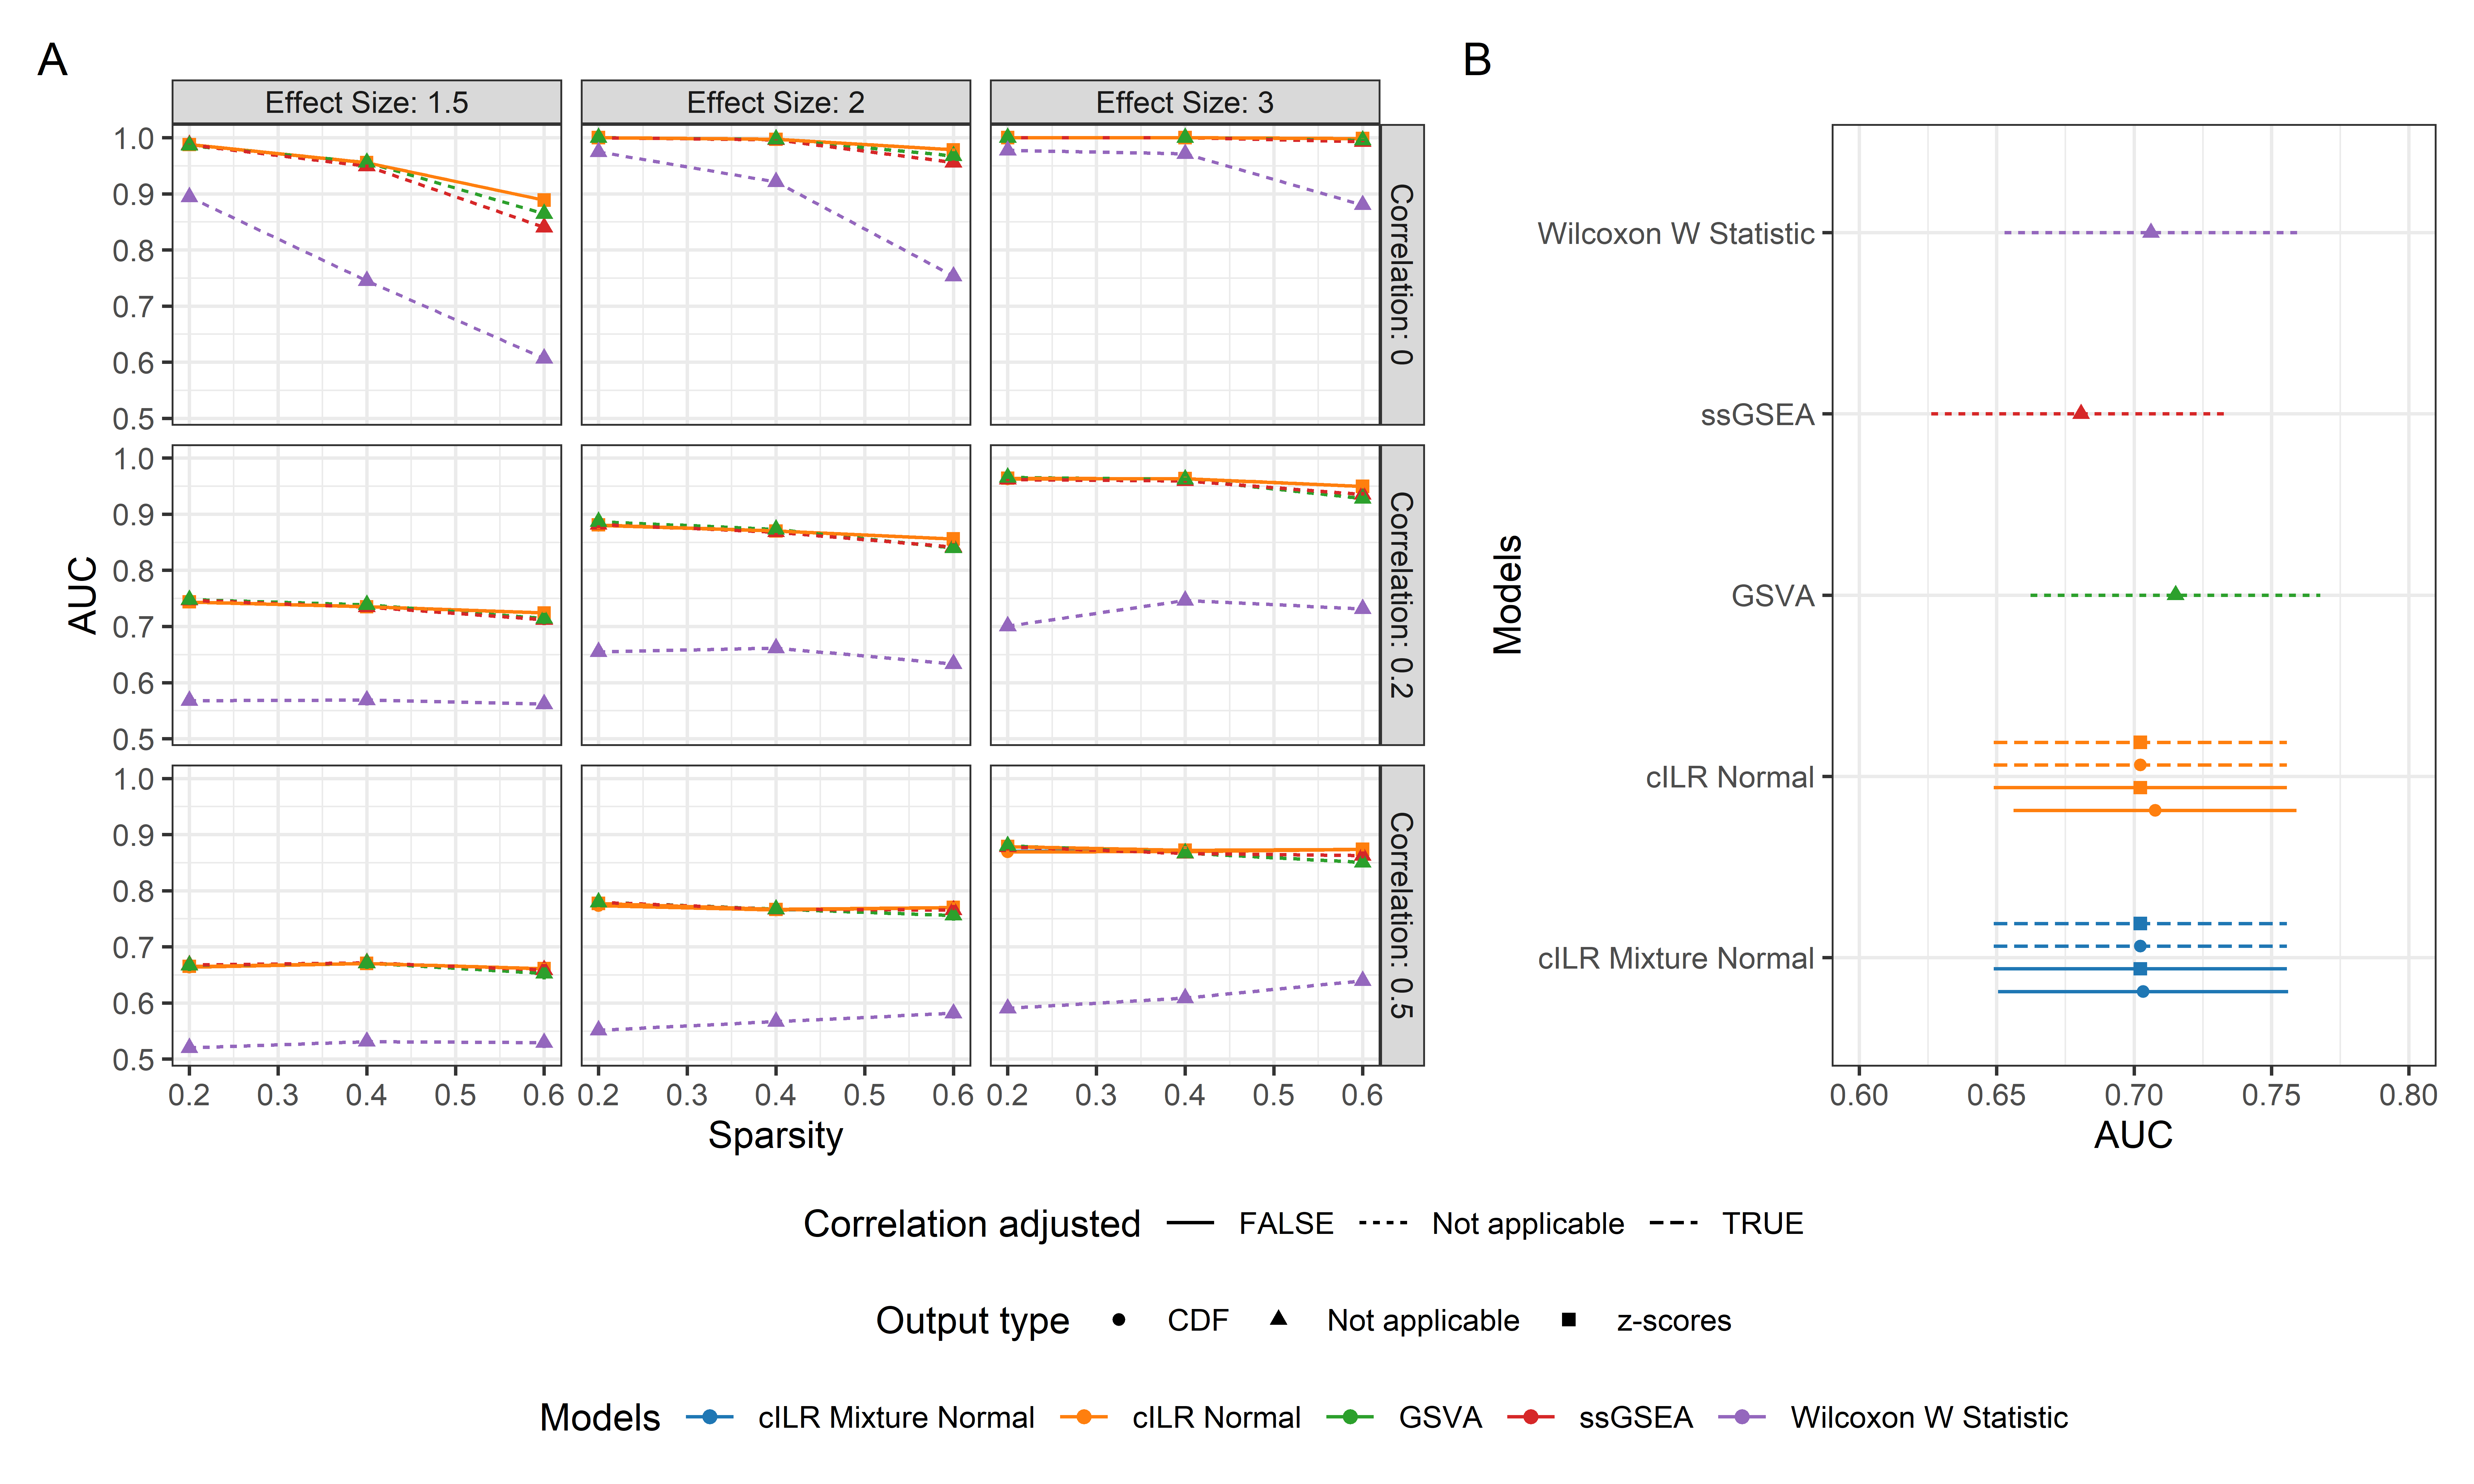
\includegraphics[width = \textwidth]{figures/sim_data_ss_auc.png}
%DIFDELCMD <     %%%
%DIFDELCMD < \caption{%
{%DIFAUXCMD
\DIFdelFL{Classification performance via AUC of cILR, ssGSEA, GSVA, and Wilcoxon $U$ statistic on simulated data }\textbf{\DIFdelFL{(A)}} %DIFAUXCMD
\DIFdelFL{the gingival data set from the Human Microbiome Project  }\textbf{\DIFdelFL{(B)}} %DIFAUXCMD
\DIFdelFL{as detailed in }%DIFDELCMD < \nameref{methods}%%%
\DIFdelFL{. Performance scores measure whether scores can highly rank samples that are known to have inflated abundance. In the gingival data set presented in panel }\textbf{\DIFdelFL{(B)}}%DIFAUXCMD
\DIFdelFL{, samples from the supragingival site are assumed to have an inflated abundance of aerobic microbes. Error bars are the 95\% DeLong confidence intervals for AUC \mbox{%DIFAUXCMD
\cite{delong1988}}\hspace{0pt}%DIFAUXCMD
}} 
    %DIFAUXCMD
%DIFDELCMD < \label{fig:3}
%DIFDELCMD < \end{figure}
%DIFDELCMD < 

%DIFDELCMD < %%%
\subsection*{\DIFdel{Differential abundance analysis}}
%DIFAUXCMD
\DIFdel{cILR generates sample-specific scores representing the degree of enrichment of a pre-defined set. As such, we want to assess the ability to use these scores for differential abundance analysis in combination with a standard difference of means statistical test (}\DIFdelend \DIFaddbegin \DIFadd{evaluate using CBEA scores generated under different settings with }\DIFaddend Welch's t-test \DIFdelbegin \DIFdel{and Wilcoxon rank sum test). We compared the performance of this approach with cILR and two commonly used methods for differential abundance testing in the microbiome literature: DESeq2 \mbox{%DIFAUXCMD
\cite{love2014} }\hspace{0pt}%DIFAUXCMD
and corncob \mbox{%DIFAUXCMD
\cite{martin2020}}\hspace{0pt}%DIFAUXCMD
}\DIFdelend \DIFaddbegin \DIFadd{in a supervised manner to assess whether a set is enriched across case/control status}\DIFaddend . 

\DIFdelbegin \subsubsection*{\DIFdel{Simulation studies}}
%DIFAUXCMD
\DIFdelend \begin{figure}[!h]
    \centering
    \DIFdelbeginFL %DIFDELCMD < 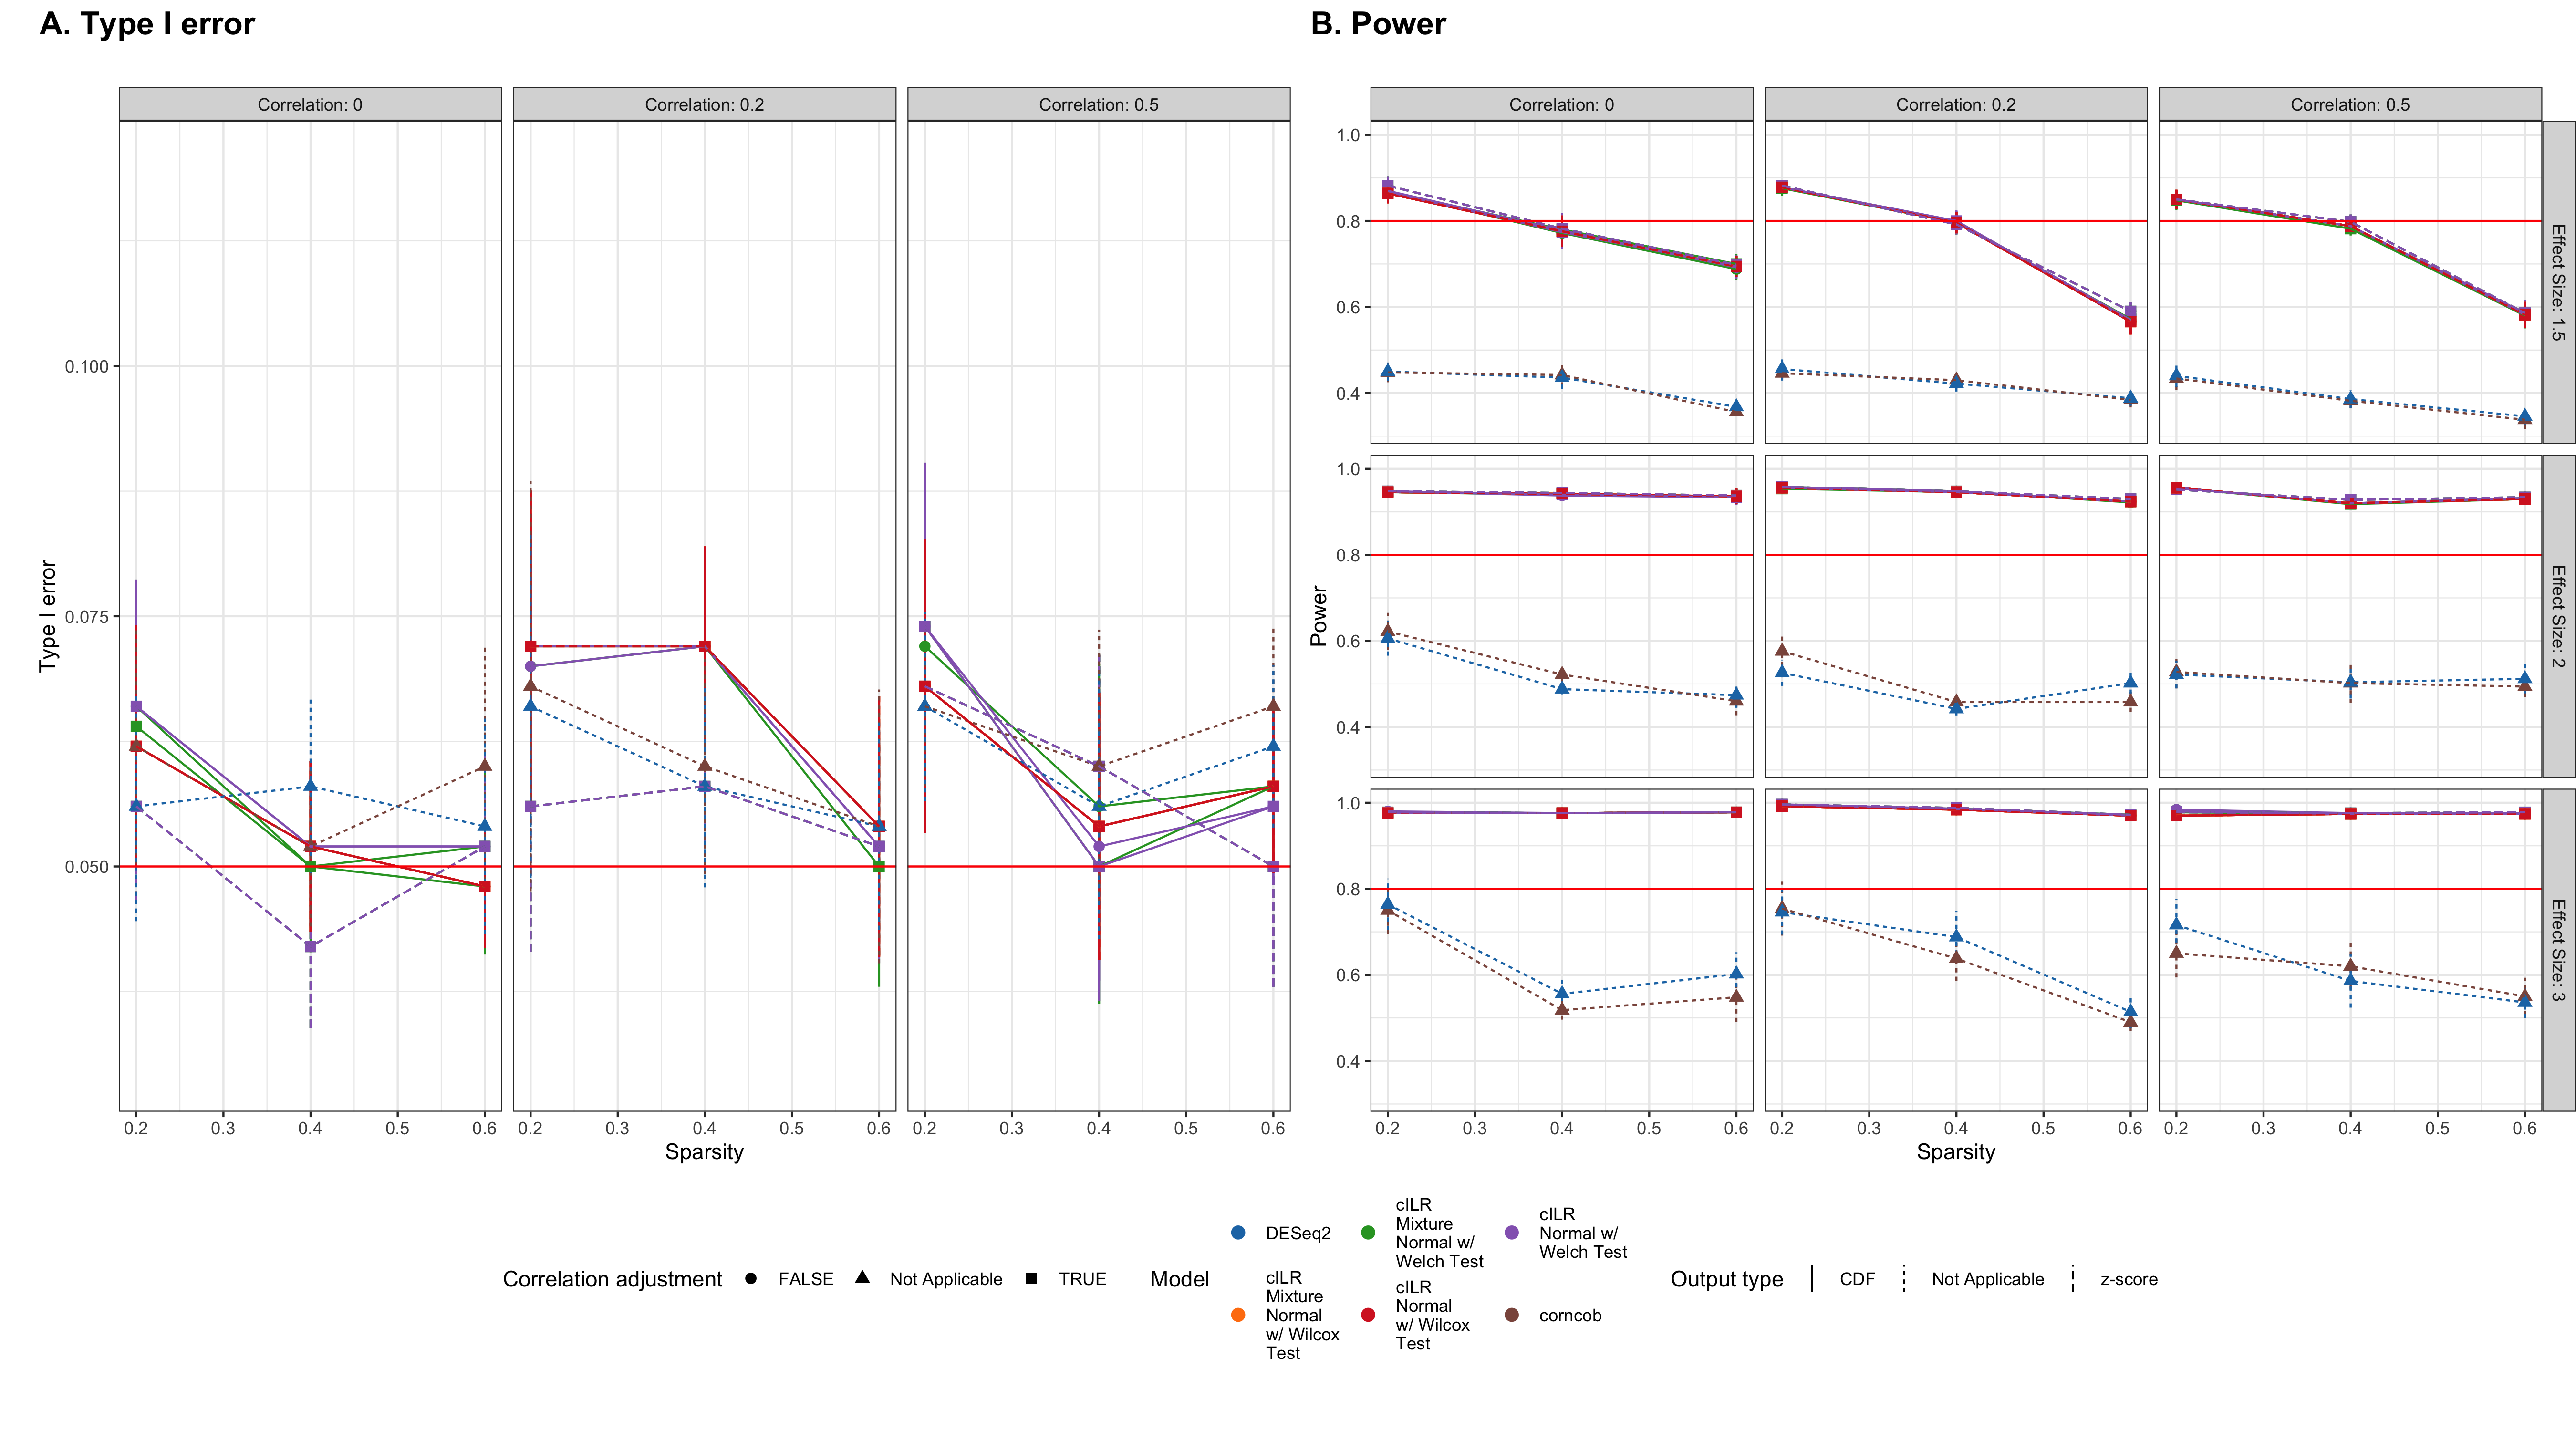
\includegraphics[width = \textwidth]{figures/sim_diff_ab_comb.png}
%DIFDELCMD <     %%%
\DIFdelendFL \DIFaddbeginFL 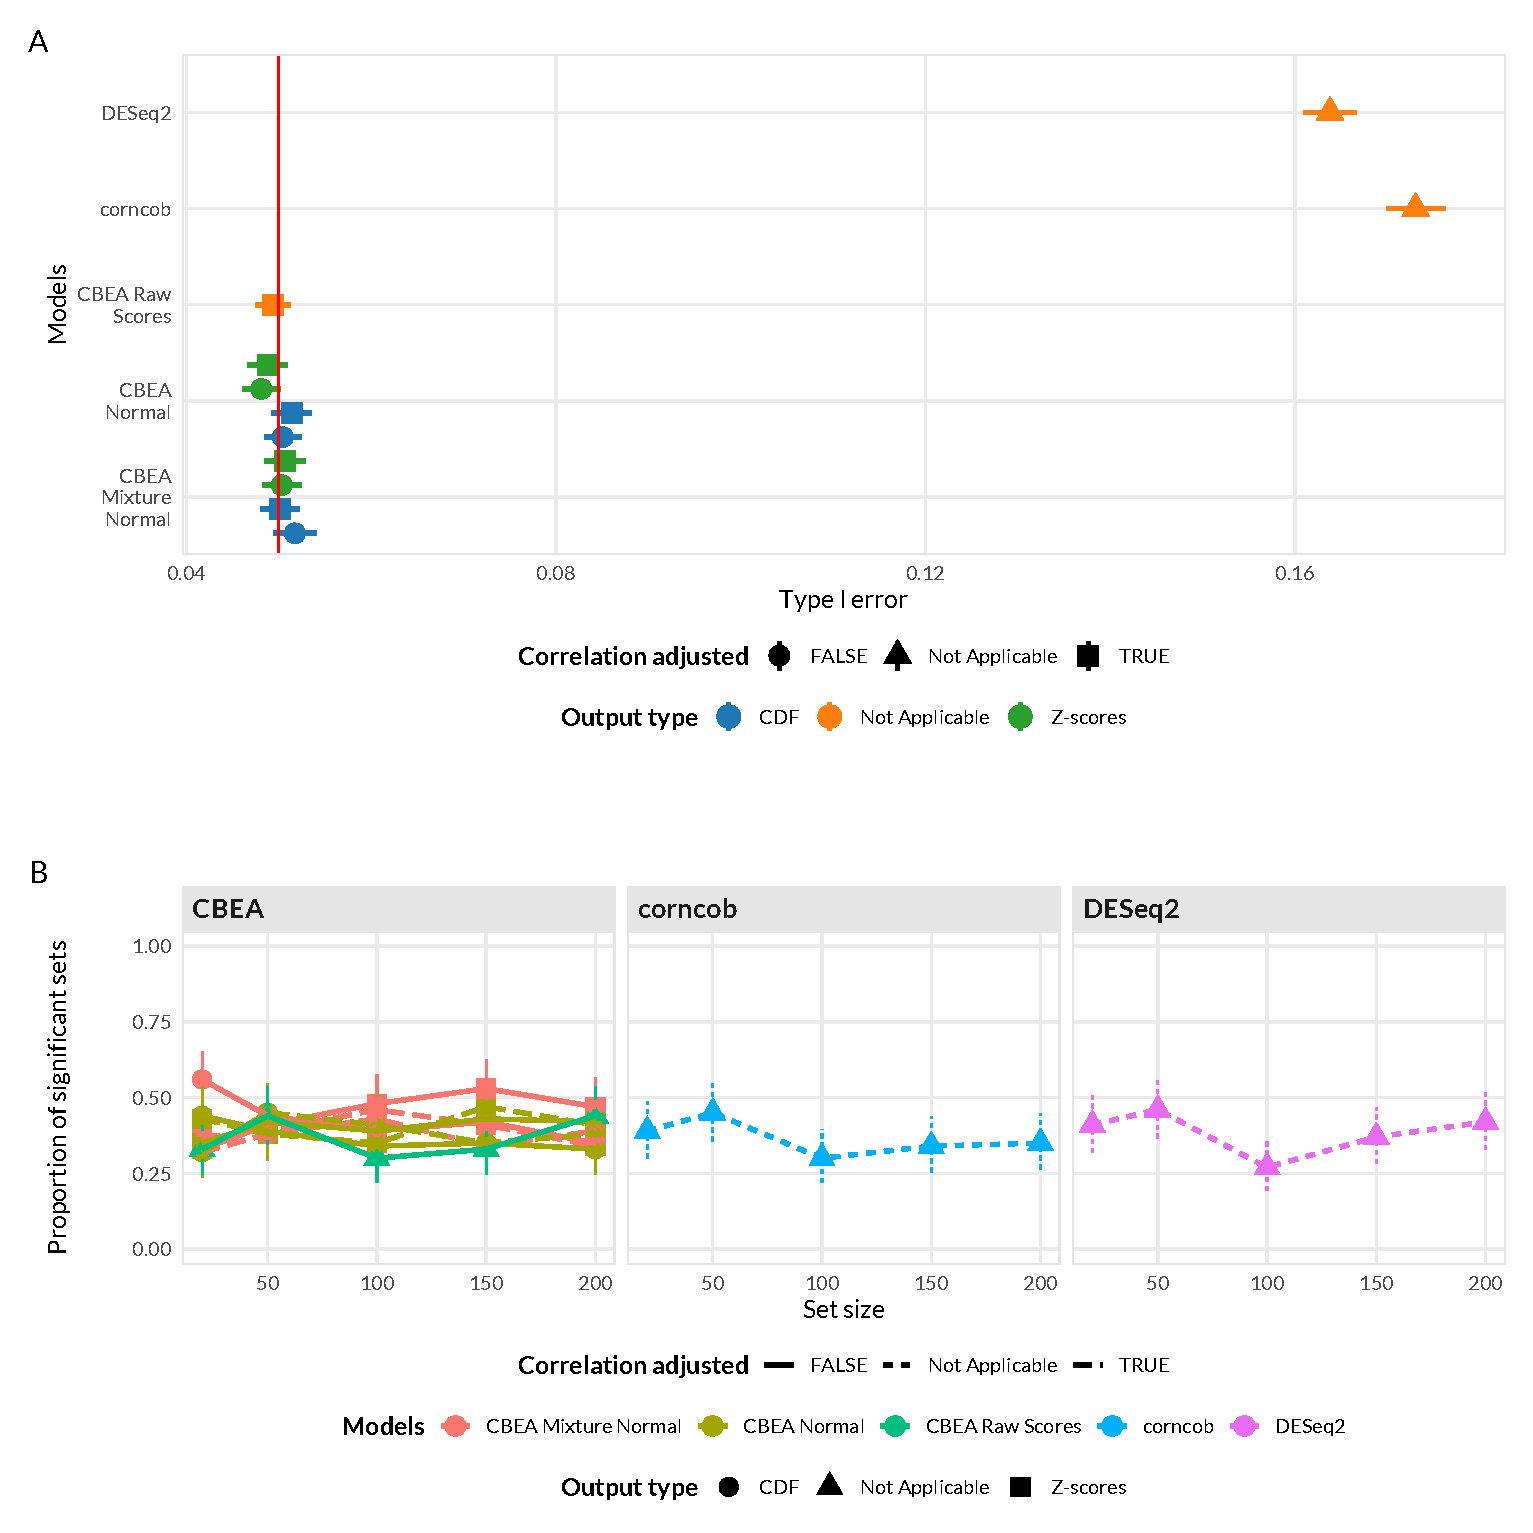
\includegraphics[width = \textwidth]{figures/data_diffab_fdr.eps}
    \DIFaddendFL \caption{\DIFdelbeginFL \DIFdelFL{Type I error rate }\textbf{\DIFdelFL{(A)}} %DIFAUXCMD
\DIFdelendFL \DIFaddbeginFL \DIFaddFL{Random sample label (}\textbf{\DIFaddFL{A}}\DIFaddFL{) }\DIFaddendFL and \DIFdelbeginFL \DIFdelFL{power }\textbf{\DIFdelFL{(B)}} %DIFAUXCMD
\DIFdelendFL \DIFaddbeginFL \DIFaddFL{random set (}\textbf{\DIFaddFL{B}}\DIFaddFL{) analyses }\DIFaddendFL for \DIFdelbeginFL \DIFdelFL{differential abundance test across different parametric simulation scenarios}\DIFdelendFL \DIFaddbeginFL \DIFaddFL{population level inference}\DIFaddendFL . \DIFdelbeginFL \DIFdelFL{For cILR methods, differential abundance analysis }\DIFdelendFL \DIFaddbeginFL \DIFaddFL{(}\textbf{\DIFaddFL{A}}\DIFaddFL{) Type I error (}\emph{\DIFaddFL{x}}\DIFaddFL{-axis) }\DIFaddendFL was \DIFdelbeginFL \DIFdelFL{performed }\DIFdelendFL \DIFaddbeginFL \DIFaddFL{estimated as the overall fraction of sets found to be enriched $\alpha = 0.05$ }\DIFaddendFL using \DIFdelbeginFL \DIFdelFL{a difference in means test }\DIFdelendFL \DIFaddbeginFL \DIFaddFL{randomly generated sample labels }\DIFaddendFL (\DIFdelbeginFL \DIFdelFL{either Wilcoxon rank-sum test or Welch's t-test}\DIFdelendFL \DIFaddbeginFL \DIFaddFL{500 permutations}\DIFaddendFL )\DIFdelbeginFL \DIFdelFL{across case/control status using single }\DIFdelendFL \DIFaddbeginFL \DIFaddFL{.  Error bars represent the mean type I error $\pm$ }\DIFaddendFL sample \DIFdelbeginFL \DIFdelFL{scores generated by cILR }\DIFdelendFL \DIFaddbeginFL \DIFaddFL{standard error. }\DIFaddendFL (\DIFdelbeginFL \DIFdelFL{across }\DIFdelendFL \DIFaddbeginFL \textbf{\DIFaddFL{B}}\DIFaddFL{) Proportion of significant sets (}\emph{\DIFaddFL{y}}\DIFaddFL{-axis) using 100 randomly generated sets of }\DIFaddendFL different \DIFdelbeginFL \DIFdelFL{output types and distributional assumptions}\DIFdelendFL \DIFaddbeginFL \DIFaddFL{set sizes (}\emph{\DIFaddFL{x}}\DIFaddFL{-axis}\DIFaddendFL ). \DIFdelbeginFL \DIFdelFL{cILR associated methods demonstrated similar }\DIFdelendFL \DIFaddbeginFL \DIFaddFL{Confidence intervals computed using Agresti-Couli method for binomial proportions. For sample label permutation (}\textbf{\DIFaddFL{A}}\DIFaddFL{), all CBEA approaches were able to control for }\DIFaddendFL type I error \DIFdelbeginFL \DIFdelFL{to conventional differential abundance analysis methods }\DIFdelendFL but \DIFdelbeginFL \DIFdelFL{with more power }\DIFdelendFL \DIFaddbeginFL \DIFaddFL{not for corncob and DESeq2. For random set analyses (}\textbf{\DIFaddFL{B}}\DIFaddFL{), all approaches demonstrate similar rate of accepting significant sets and were invariant }\DIFaddendFL to \DIFdelbeginFL \DIFdelFL{detect differences even at small effect sizes}\DIFdelendFL \DIFaddbeginFL \DIFaddFL{overall set size}\DIFaddendFL .}  
    \DIFdelbeginFL %DIFDELCMD < \label{fig:4}
%DIFDELCMD < %%%
\DIFdelendFL \DIFaddbeginFL \label{fig:3}
\DIFaddendFL \end{figure}

Fig\DIFdelbegin \DIFdel{.~\ref{fig:4} present results for simulation studies for both type I error (panel A) and power (panel B) evaluations. All methods }\DIFdelend \DIFaddbegin \DIFadd{~\ref{fig:3} shows results for this scenario using both random sample label and random set evaluations. The random sample label approach (Fig~\ref{fig:3}A) provides a controlled setting where we can estimate type I error rate controlled at $\alpha = 0.05$. Across all replications, CBEA methods were able to }\DIFaddend control for type I error \DIFdelbegin \DIFdel{well across both sparsity and correlation levels, where the estimated rate was consistently around the }\DIFdelend \DIFaddbegin \DIFadd{at the nominal threshold of }\DIFaddend 0.05\DIFdelbegin \DIFdel{pre-defined threshold . Results were similar across all evaluated methods, although in some instances, for example in medium correlation setting ($\rho = 0.2$), the unadjusted cILR resulted in higher }\DIFdelend \DIFaddbegin \DIFadd{, with CBEA raw scores being the most performant. Neither output types, correlation adjustment, nor distributional assumption improved performance values. Surprisingly, DESeq2 and corncob both exhibit significantly inflated }\DIFaddend type I error\DIFdelbegin \DIFdel{, regardless of difference in means test and distribution of choice}\DIFdelend . 

\DIFdelbegin \DIFdel{The difference between the methods is more noticeable when evaluating power. All cILR associated variants showed much higher power even when the effect size is limited (fold change is 1.5), and there is a noticeable gap in performance between cILR and both }\DIFdelend \DIFaddbegin \DIFadd{We also assessed the impact of set-size on the inference procedure by testing for enrichment using the original sample labels but with randomly sampled sets of different sizes (Fig~\ref{fig:3}B). Overall we observed very similar values across CBEA as well as corncob and }\DIFaddend DESeq2\DIFdelbegin \DIFdel{and corncob. Surprisingly, this effect is consistent across correlation levels and sparsity, even though we expectedly see performance in power drop as a function of sparsity especially in low effect size settings}\DIFdelend \DIFaddbegin \DIFadd{, suggesting that no individual method is systematically identifying too many significant sets. Additionally, similar to analogous analyses at the sample level, no approach were significantly sensitive to changes in set sizes}\DIFaddend .  

\DIFaddbegin \subsection*{\DIFadd{Phenotype Relevance}} 
\DIFaddend \subsubsection*{\DIFdelbegin \DIFdel{Real data evaluations}%DIFDELCMD < \MBLOCKRIGHTBRACE
%DIFDELCMD < %%%
\DIFdel{In addition to simulation studies, we also evaluated performance of the methods on real 16S rRNA gene sequencing data set from HMP (Fig~\ref{fig:5}). For type I error evaluations, we use stool samples and randomly assign them with case/control status and calculated type I error as the proportion of genera identified as significantly different. For true positive rate evaluations, we use }\DIFdelend \DIFaddbegin \DIFadd{Inference at }\DIFaddend the \DIFaddbegin \DIFadd{sample level}}
\begin{figure}[!h]
    \centering
    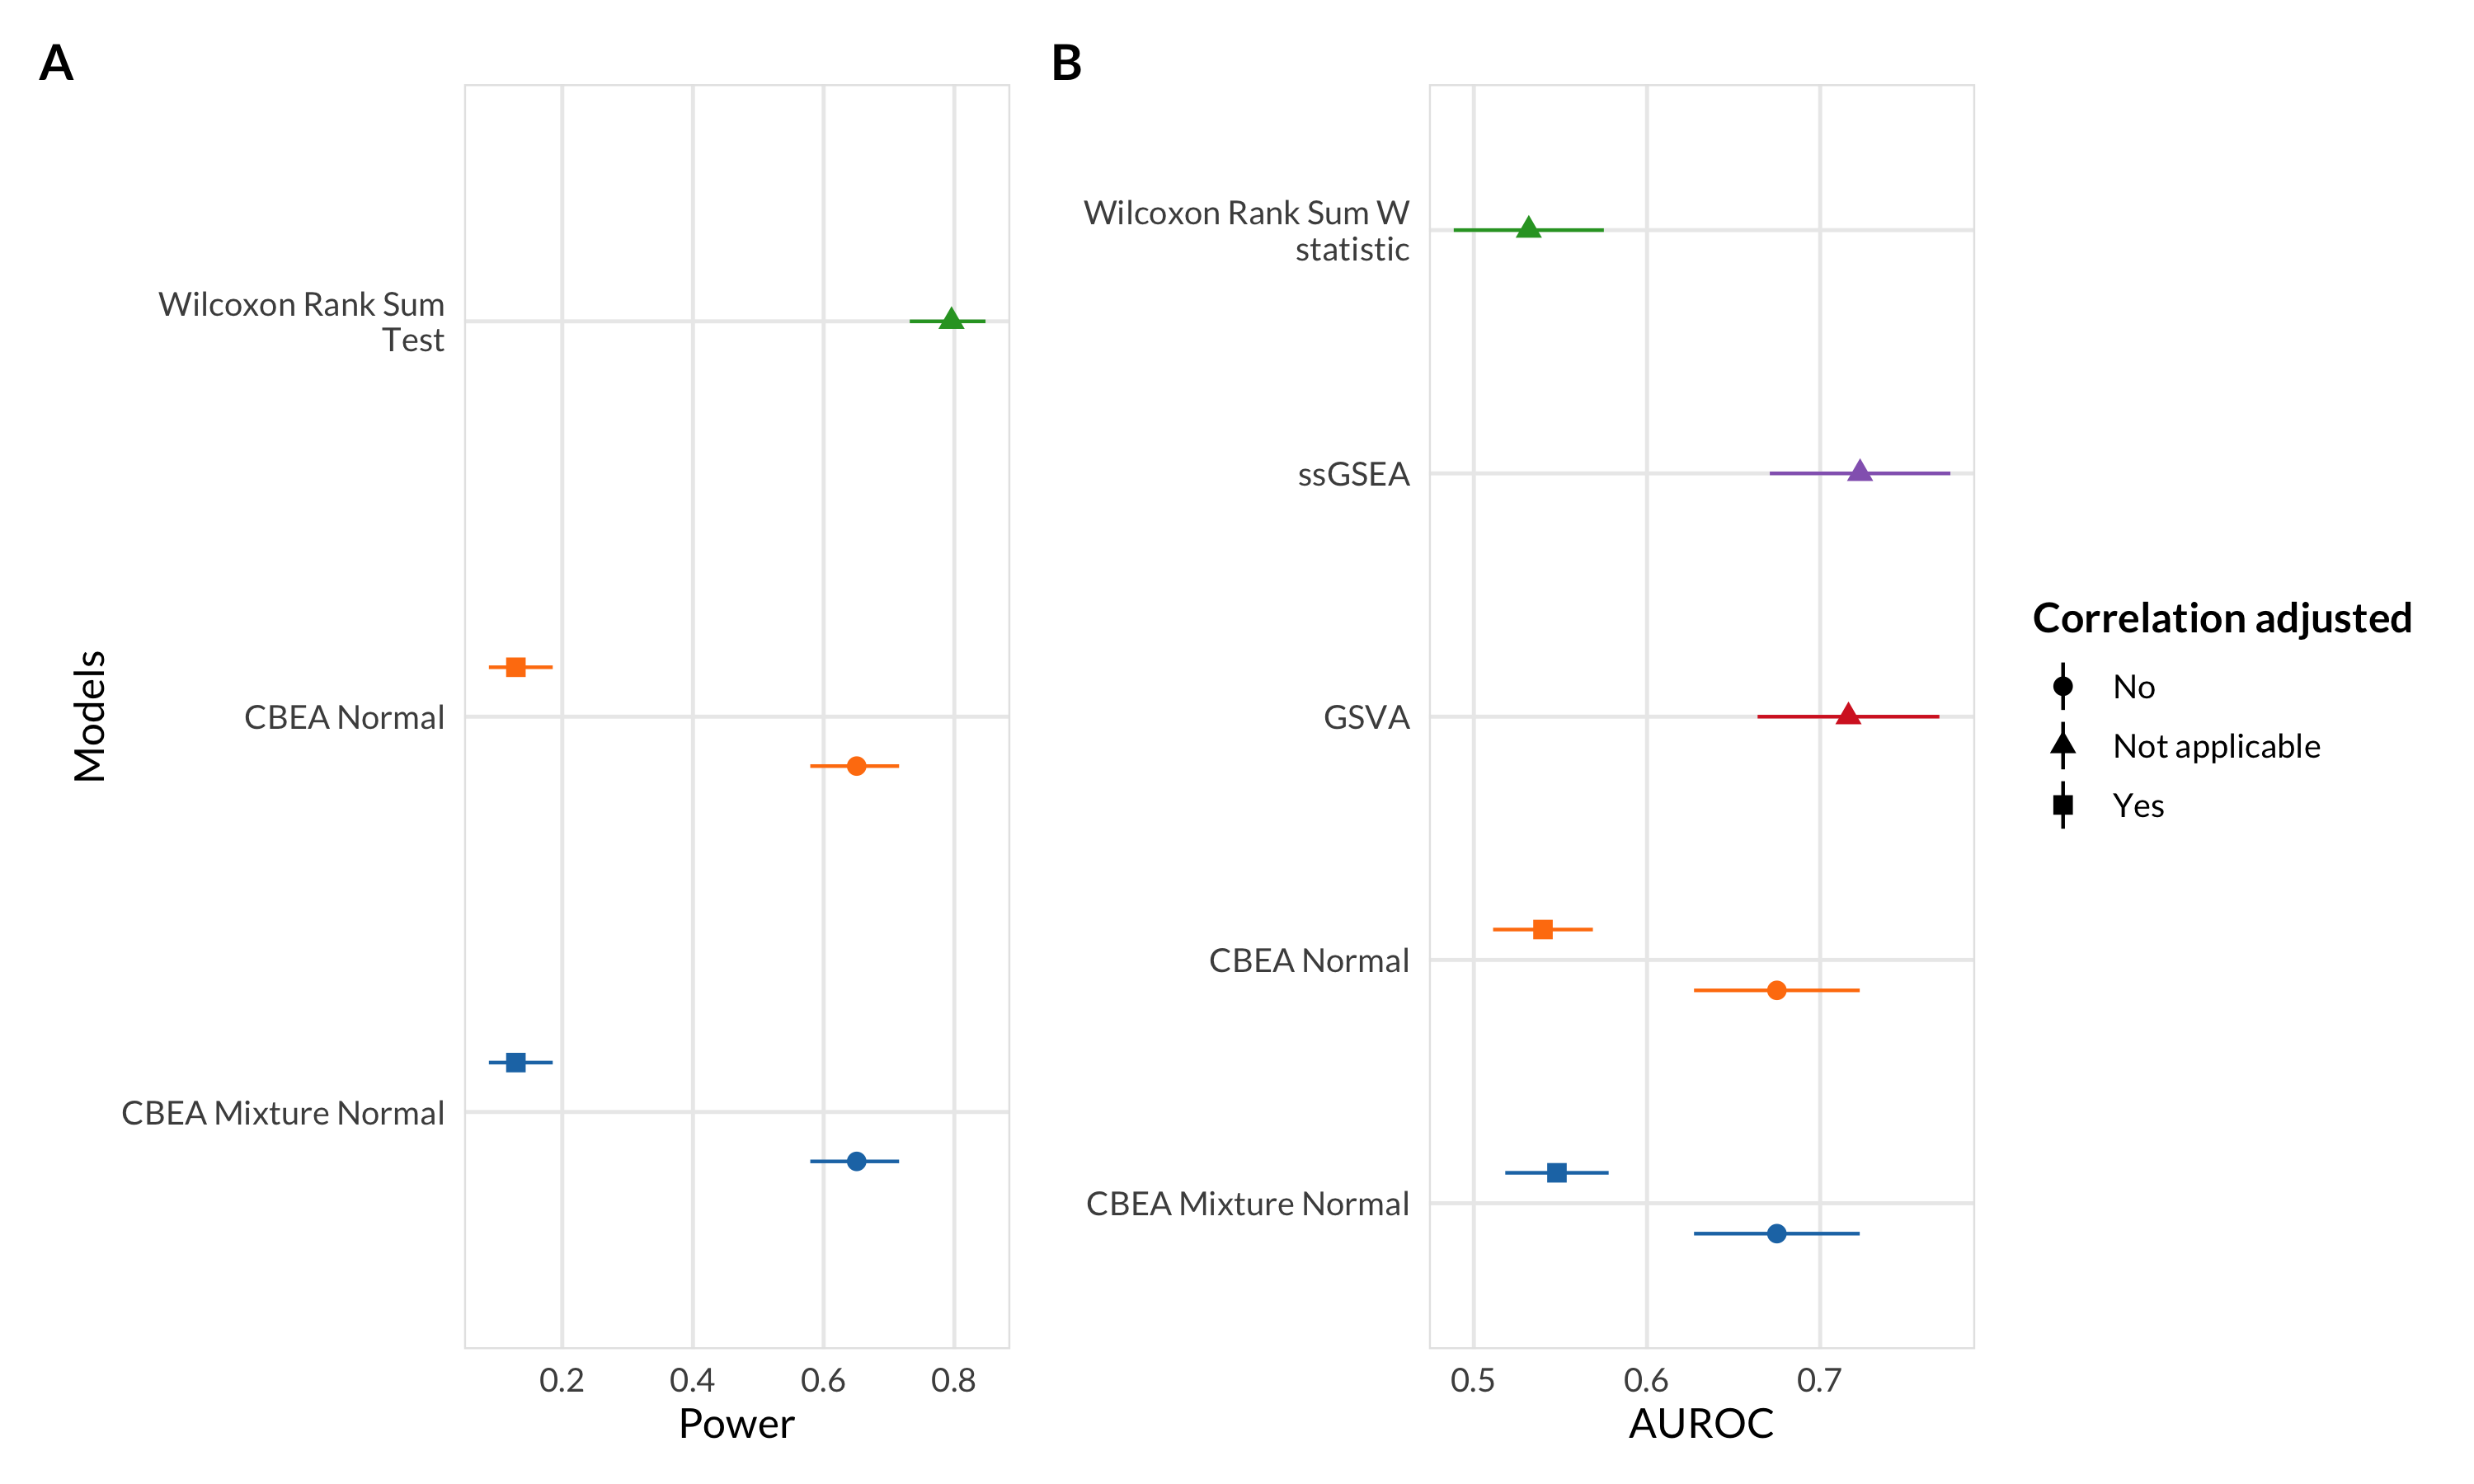
\includegraphics[width = \textwidth]{figures/data_ss_pwr_new.png}
    \caption{\DIFaddFL{Statistical power (}\textbf{\DIFaddFL{A}}\DIFaddFL{) and score rankings (}\textbf{\DIFaddFL{B}}\DIFaddFL{) to assess phenotype relevance. (}\textbf{\DIFaddFL{A}}\DIFaddFL{) Power (}\emph{\DIFaddFL{x}}\DIFaddFL{-axis) was estimated as the overall fraction of aerobic microbes found to be enriched in supragingival samples at $\alpha = 0.05$. 95\% confidence intervals were computed using the Agresti-Couli approach for binomial proportions. (}\textbf{\DIFaddFL{B}}\DIFaddFL{) Score rankings were evaluated by comparing computed scores against true values using AUROC (}\emph{\DIFaddFL{x}}\DIFaddFL{-axis). DeLong 95 \% confidence intervals for AUROC were computed.}} 
    \label{fig:4}
\end{figure}

\DIFadd{In Fig~\ref{fig:4}, we evaluate whether sets found to be significant by CBEA are relevant to the phenotype of interest. We leveraged the }\DIFaddend gingival data set as \DIFdelbegin \DIFdel{detailed in the previous section , and calculated the true positive rate as the proportion of genera labeled as either anaerobic or aerobic that were found to be significant. }%DIFDELCMD < 

%DIFDELCMD < %%%
\DIFdel{We observed both corncob and DESeq2 had significantly inflated type I error rate while all variations of cILR were controlling for type I error at the defined $\alpha$ threshold of 0.05}\DIFdelend \DIFaddbegin \DIFadd{stated in }\nameref{evaluation} \DIFadd{section where we know beforehand that aerobic microbes are more likely to be enriched in supragingival subsite samples and vice versa. 
}

\DIFadd{We estimated statistical power using this data set as the fraction of supragingival samples where the set representing aerobic microbes were significantly enriched. We observed that adjusted CBEA approaches demonstrate much lower power compared to the Wilcoxon rank-sum test and unadjusted variants}\DIFaddend . This is surprising given the \DIFdelbegin \DIFdel{consistency of preserving }\DIFdelend \DIFaddbegin \DIFadd{fact that in statistical significance analyses, the adjusted CBEA approach provides inflated }\DIFaddend type I error\DIFdelbegin \DIFdel{for both corncob and DESeq2 in all simulation evaluations}\DIFdelend \DIFaddbegin \DIFadd{, especially if the normal distribution assumption was chosen, which indicates a mismatch in estimating the null distribution since a high type I error did not result in increased power}\DIFaddend . 

\DIFdelbegin \DIFdel{In true positive experiments with data from the gingival site, estimated rates were more similar across the different methods. As expected, }\DIFdelend \DIFaddbegin \DIFadd{We also evaluated phenotype relevance by assessing whether enriched sets according to ground truth are preferentially ranked higher using assigned continuous scores (instead of performing a hypothesis test). This aspect is captured through computing AUROC values comparing computed enrichment scores and true labels. Consistent with prior approaches, adjusting for correlation did not improve performance, where the AUROC values are equivalent to }\DIFaddend using the Wilcoxon \DIFdelbegin \DIFdel{rank sum test resulted in lower true positive rate compared to remaining methods , but the difference was not noticable.  
This is also surprising given that }\DIFdelend \DIFaddbegin \DIFadd{Rank sum statistic at around 0.5. Unadjusted methods were much better at ranking true enriched sets, however the mean AUROC values are lower than alternate single sample enrichment methods (GSVA \mbox{%DIFAUXCMD
\cite{hanzelmann2013} }\hspace{0pt}%DIFAUXCMD
and ssGSEA \mbox{%DIFAUXCMD
\cite{barbie2009}}\hspace{0pt}%DIFAUXCMD
) even though this difference is not significant due to overlapping confidence intervals.  
}

\DIFadd{The above results were replicated }\DIFaddend in simulation studies \DIFdelbegin \DIFdel{, both corncob and DESeq2 showed markedly lower power across all }\DIFdelend \DIFaddbegin \DIFadd{where we observed that adjusted approaches was very conservative and demonstrated significantly lower power (}\nameref{S3_Fig}\DIFadd{) with increasing correlation even at the highest evaluated }\DIFaddend effect sizes. \DIFaddbegin \DIFadd{When assessing score rankings, the performance of CBEA was closer to ssGSEA and GSVA compared to real data evaluations, however all single sample approaches were much better than using the W statistic from the Wilcoxon Rank Sum test.   
}\DIFaddend 

\DIFaddbegin \subsubsection*{\DIFadd{Inference at the population level}}
\DIFaddend \begin{figure}[!h]
    \centering
    \DIFdelbeginFL %DIFDELCMD < 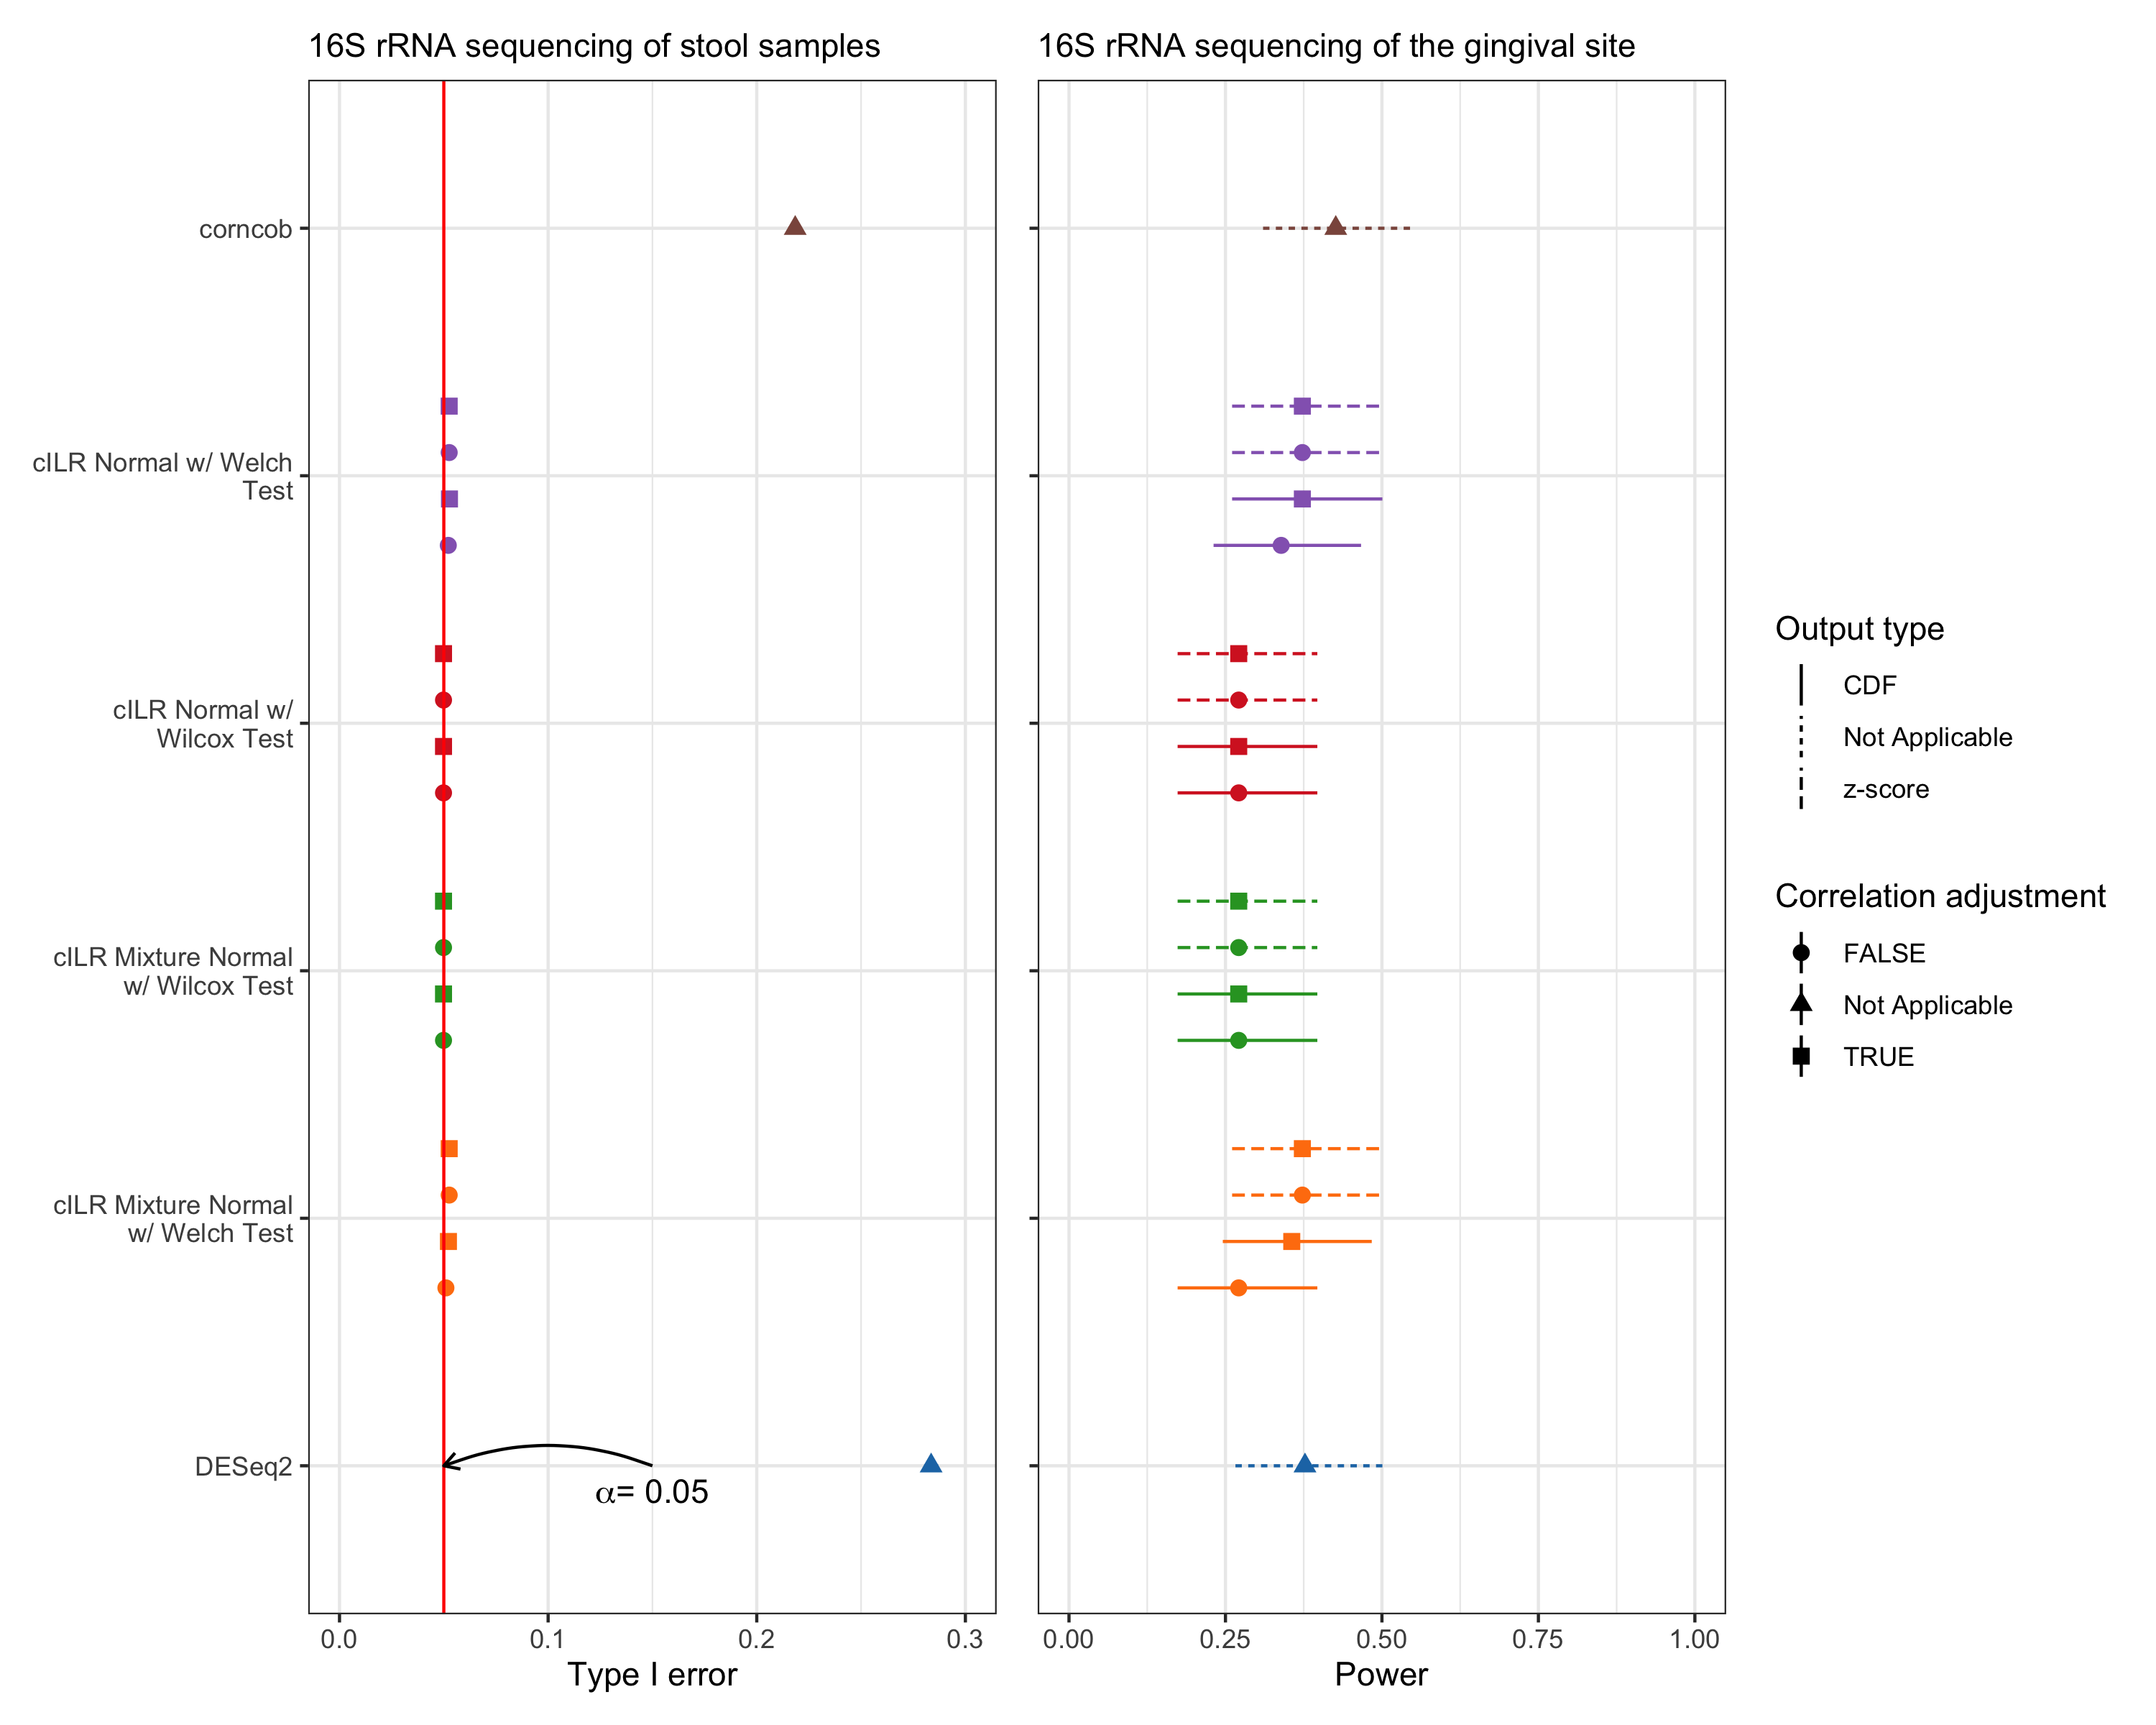
\includegraphics[width = \textwidth]{figures/data_diff_ab.png}
%DIFDELCMD <     %%%
\DIFdelendFL \DIFaddbeginFL 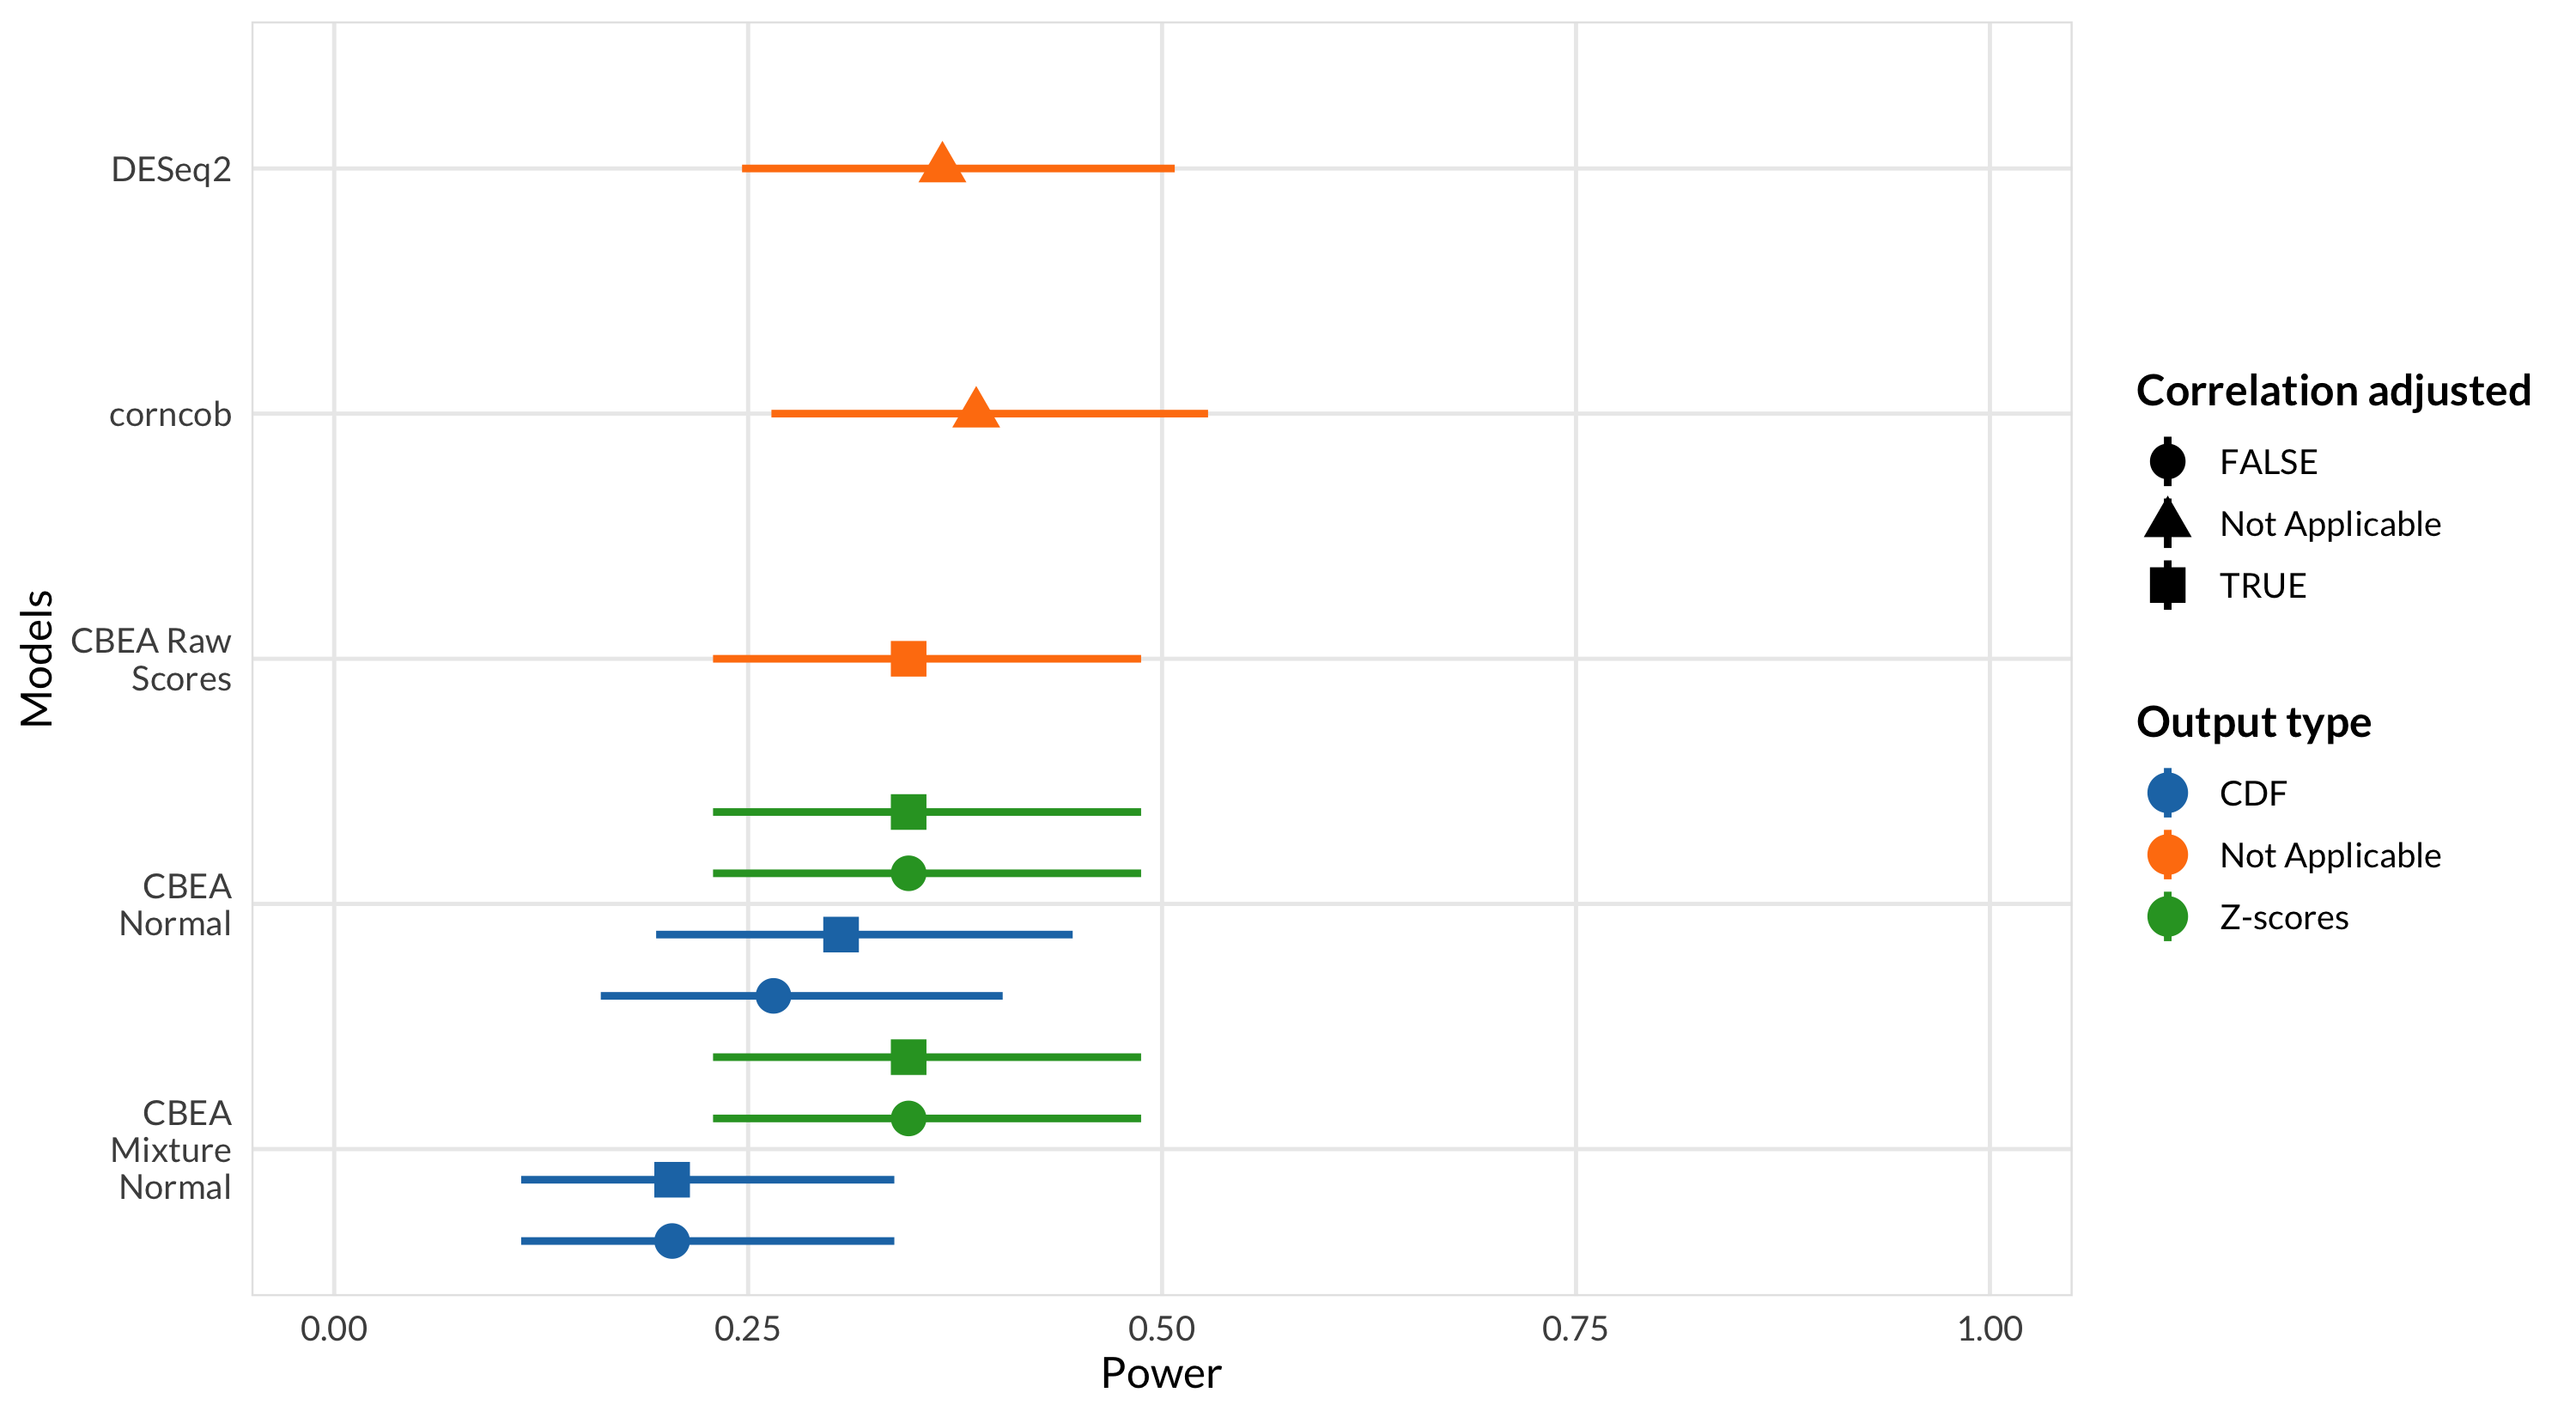
\includegraphics[width = \textwidth]{figures/data_diffab_pwr.png}
    \DIFaddendFL \caption{\DIFdelbeginFL \DIFdelFL{Differential abundance analysis using corncob, DESeq2 and cILR with either Wilcoxon rank sum test or Welch's t-test. Panel }\textbf{\DIFdelFL{(A)}} %DIFAUXCMD
\DIFdelFL{shows type I error results as the proportion of significant genera after 500 iterations where case/control status was assigned randomly }\DIFdelendFL \DIFaddbeginFL \DIFaddFL{Statistical power }\DIFaddendFL to \DIFdelbeginFL \DIFdelFL{each sample}\DIFdelendFL \DIFaddbeginFL \DIFaddFL{assess phenotype relevance of inference tasks at the population level}\DIFaddendFL . \DIFdelbeginFL \DIFdelFL{Panel }\textbf{\DIFdelFL{(B)}} %DIFAUXCMD
\DIFdelFL{shows true positive rate results }\DIFdelendFL \DIFaddbeginFL \DIFaddFL{Power (}\emph{\DIFaddFL{x}}\DIFaddFL{-axis) was estimated }\DIFaddendFL as the \DIFdelbeginFL \DIFdelFL{proportion }\DIFdelendFL \DIFaddbeginFL \DIFaddFL{overall fraction }\DIFaddendFL of \DIFdelbeginFL \DIFdelFL{significant }\DIFdelendFL \DIFaddbeginFL \DIFaddFL{sets representing }\DIFaddendFL genera \DIFdelbeginFL \DIFdelFL{who }\DIFdelendFL \DIFaddbeginFL \DIFaddFL{that }\DIFaddendFL are \DIFdelbeginFL \DIFdelFL{either obligate anaerobes }\DIFdelendFL \DIFaddbeginFL \DIFaddFL{aerobic }\DIFaddendFL or \DIFdelbeginFL \DIFdelFL{aerobes}\DIFdelendFL \DIFaddbeginFL \DIFaddFL{anaerobic microbes found to be differentially enriched across sample type (supragingival or subgingival)}\DIFaddendFL . \DIFdelbeginFL \DIFdelFL{Both evaluations use 16S rRNA gene sequencing data from HMP. Type I error evaluation used stool samples while }\DIFdelendFL \DIFaddbeginFL \DIFaddFL{95\% confidence intervals were computed using }\DIFaddendFL the \DIFdelbeginFL \DIFdelFL{true positive rate evaluation used samples from the gingival site}\DIFdelendFL \DIFaddbeginFL \DIFaddFL{Agresti-Couli approach for binomial proportions}\DIFaddendFL .\DIFdelbeginFL \DIFdelFL{Results showed that cILR associated methods were able to keep type I error rate at approximately 0.05 while still demonstrating similar power as both corncob and DESeq2}\DIFdelendFL }  
    \label{fig:5}
\end{figure}

\DIFaddbegin \DIFadd{We also assessed statistical power for population level inference scenarios using a similar approach. Here, enrichment scores for sets representing all identified genera were computed, and estimated power as the fraction of sets found to be differentially enriched across sample site labels (supragingival or subgingival). We compared these results against performing a differential abundance test of genus level features generated via sum-based approaches. Results are shown in Fig~\ref{fig:5}. Some CBEA variants, such as CDF outputs for the mixture normal distributional assumption, did not correctly detect as many significant sets as DESeq2 or corncob despite very close performance values. Using raw CBEA scores was best approach, however it did not exceed values obtained from DESeq2 and corncob. 
}

\DIFaddend \subsection*{Disease Prediction}   
Since \DIFdelbegin \DIFdel{cILR }\DIFdelend \DIFaddbegin \DIFadd{CBEA }\DIFaddend can generate informative scores that can discriminate between samples with inflated counts for a set (Fig~\DIFdelbegin \DIFdel{\ref{fig:2}}\DIFdelend \DIFaddbegin \DIFadd{\ref{fig:4}}\DIFaddend ), we want to assess whether they can also act as useful inputs to predictive models. In this section we assessed the predictive performance of a \DIFdelbegin \DIFdel{naive }\DIFdelend \DIFaddbegin \DIFadd{standard baseline }\DIFaddend random forest model \cite{breiman2001} with different single sample enrichment scoring methods as inputs (\DIFdelbegin \DIFdel{evaluating cILR}\DIFdelend \DIFaddbegin \DIFadd{CBEA}\DIFaddend , ssGSEA, and GSVA). Additionally, we also compared predictive performance of using these scores against the a standard approach of using the centered log ratio transformation (CLR) on taxon sets aggregated via abundance summations.     
\DIFdelbegin \subsubsection*{\DIFdel{Simulation studies}}
%DIFAUXCMD
\DIFdel{Fig~\ref{fig:6} shows results for simulation studies as detailed in the }%DIFDELCMD < \nameref{methods} %%%
\DIFdel{section. Panel A presents results for a regression learning task with a continuous outcome while panel B presents results for a classification task with a binary outcome. As expected, performance across all assessed methods increased with a higher signal-to-noise ratio. Both CLR and cILR approaches outperformed both GSVA and ssGSEA across all simulation conditions and learning tasks. This is because both GSVA and ssGSEA are more sensitive to the degree of inter-taxa correlation and sparsity, while cILR and CLR did not experience a similar level of impact. As such, performance gap widens with increasing correlation and sparsity. Interestingly, this difference in performance is not as pronounced under high levels of effect saturation (across both learning tasks), suggesting that when there is a high number of sets contributing to an effect, model choice might not be as important.   
}\DIFdelend 

\DIFdelbegin \DIFdel{In this analysis, cILR unfortunately did not outperform the CLR approach, which is standard practice within the microbiome literature \mbox{%DIFAUXCMD
\cite{gloor2017}}\hspace{0pt}%DIFAUXCMD
. This difference in performance is more notable in regression learning tasks compared to classification, and at lower levels of effect saturation. However, the degree of separation between the two approaches is not as dramatic as between GSVA/ssGSEA and cILR/CLR. Moreover, the performance gap decreases with increasing effect signal-to-noise ratio and sparsity. Additionally, we did not observe any performance difference between the different variations of cILR. 
}%DIFDELCMD < 

%DIFDELCMD < \begin{figure}[!h]
%DIFDELCMD <     \centering
%DIFDELCMD <     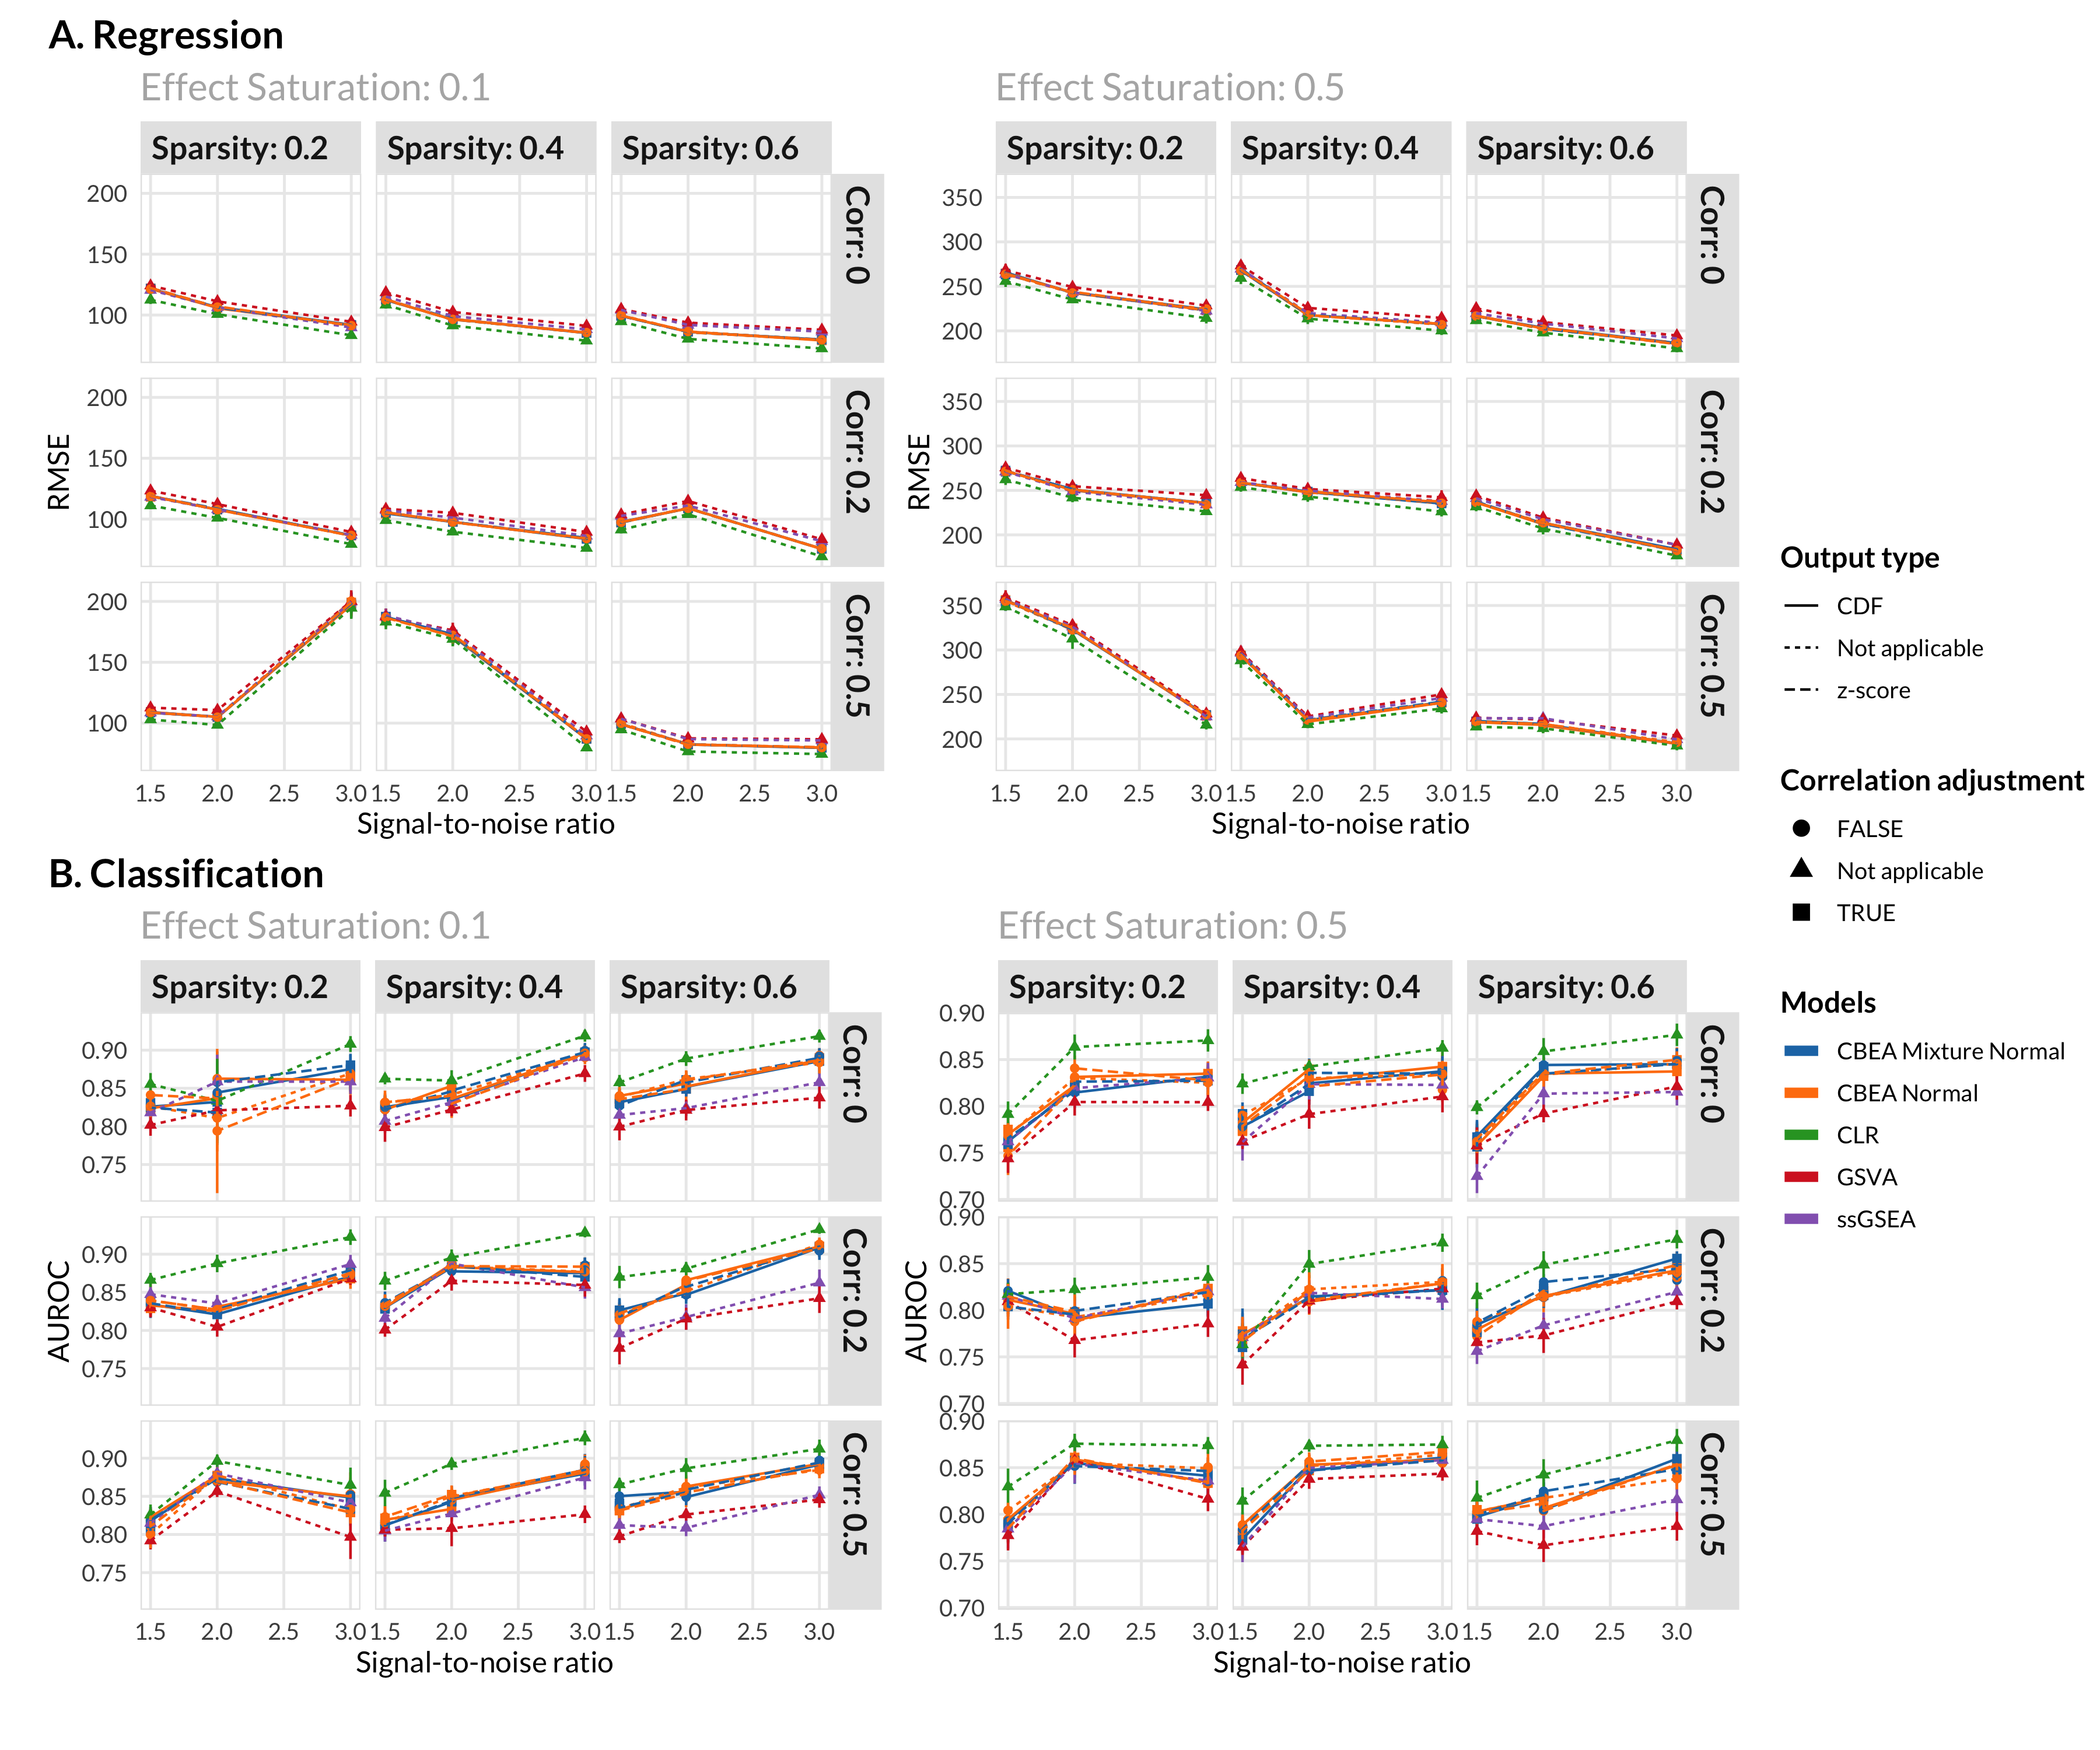
\includegraphics[width = \linewidth]{figures/sim_pred_combined.png}
%DIFDELCMD <     %%%
%DIFDELCMD < \caption{%
{%DIFAUXCMD
\DIFdelFL{Predictive performance of a naive random forest model trained on cILR, ssGSEA, GSVA generated scores as well as the standard CLR approach on simulated across different levels of data sparsity, inter-taxa correlation, effect saturation, and signal-to-noise ratio. Panel }\textbf{\DIFdelFL{(A)}} %DIFAUXCMD
\DIFdelFL{presents performance on a regression task using predictive R-squared as the evaluation measure. Panel }\textbf{\DIFdelFL{(B)}} %DIFAUXCMD
\DIFdelFL{presents performance on a classification task with AUC as the evaluation measure. cILR approaches outperformed GSVA and ssGSEA across all simulation conditions but not the CLR approach.}}
    %DIFAUXCMD
%DIFDELCMD < \label{fig:6}
%DIFDELCMD < \end{figure}
%DIFDELCMD < 

%DIFDELCMD < %%%
\DIFdelend %\begin{figure}[!ht]
%    \centering
%    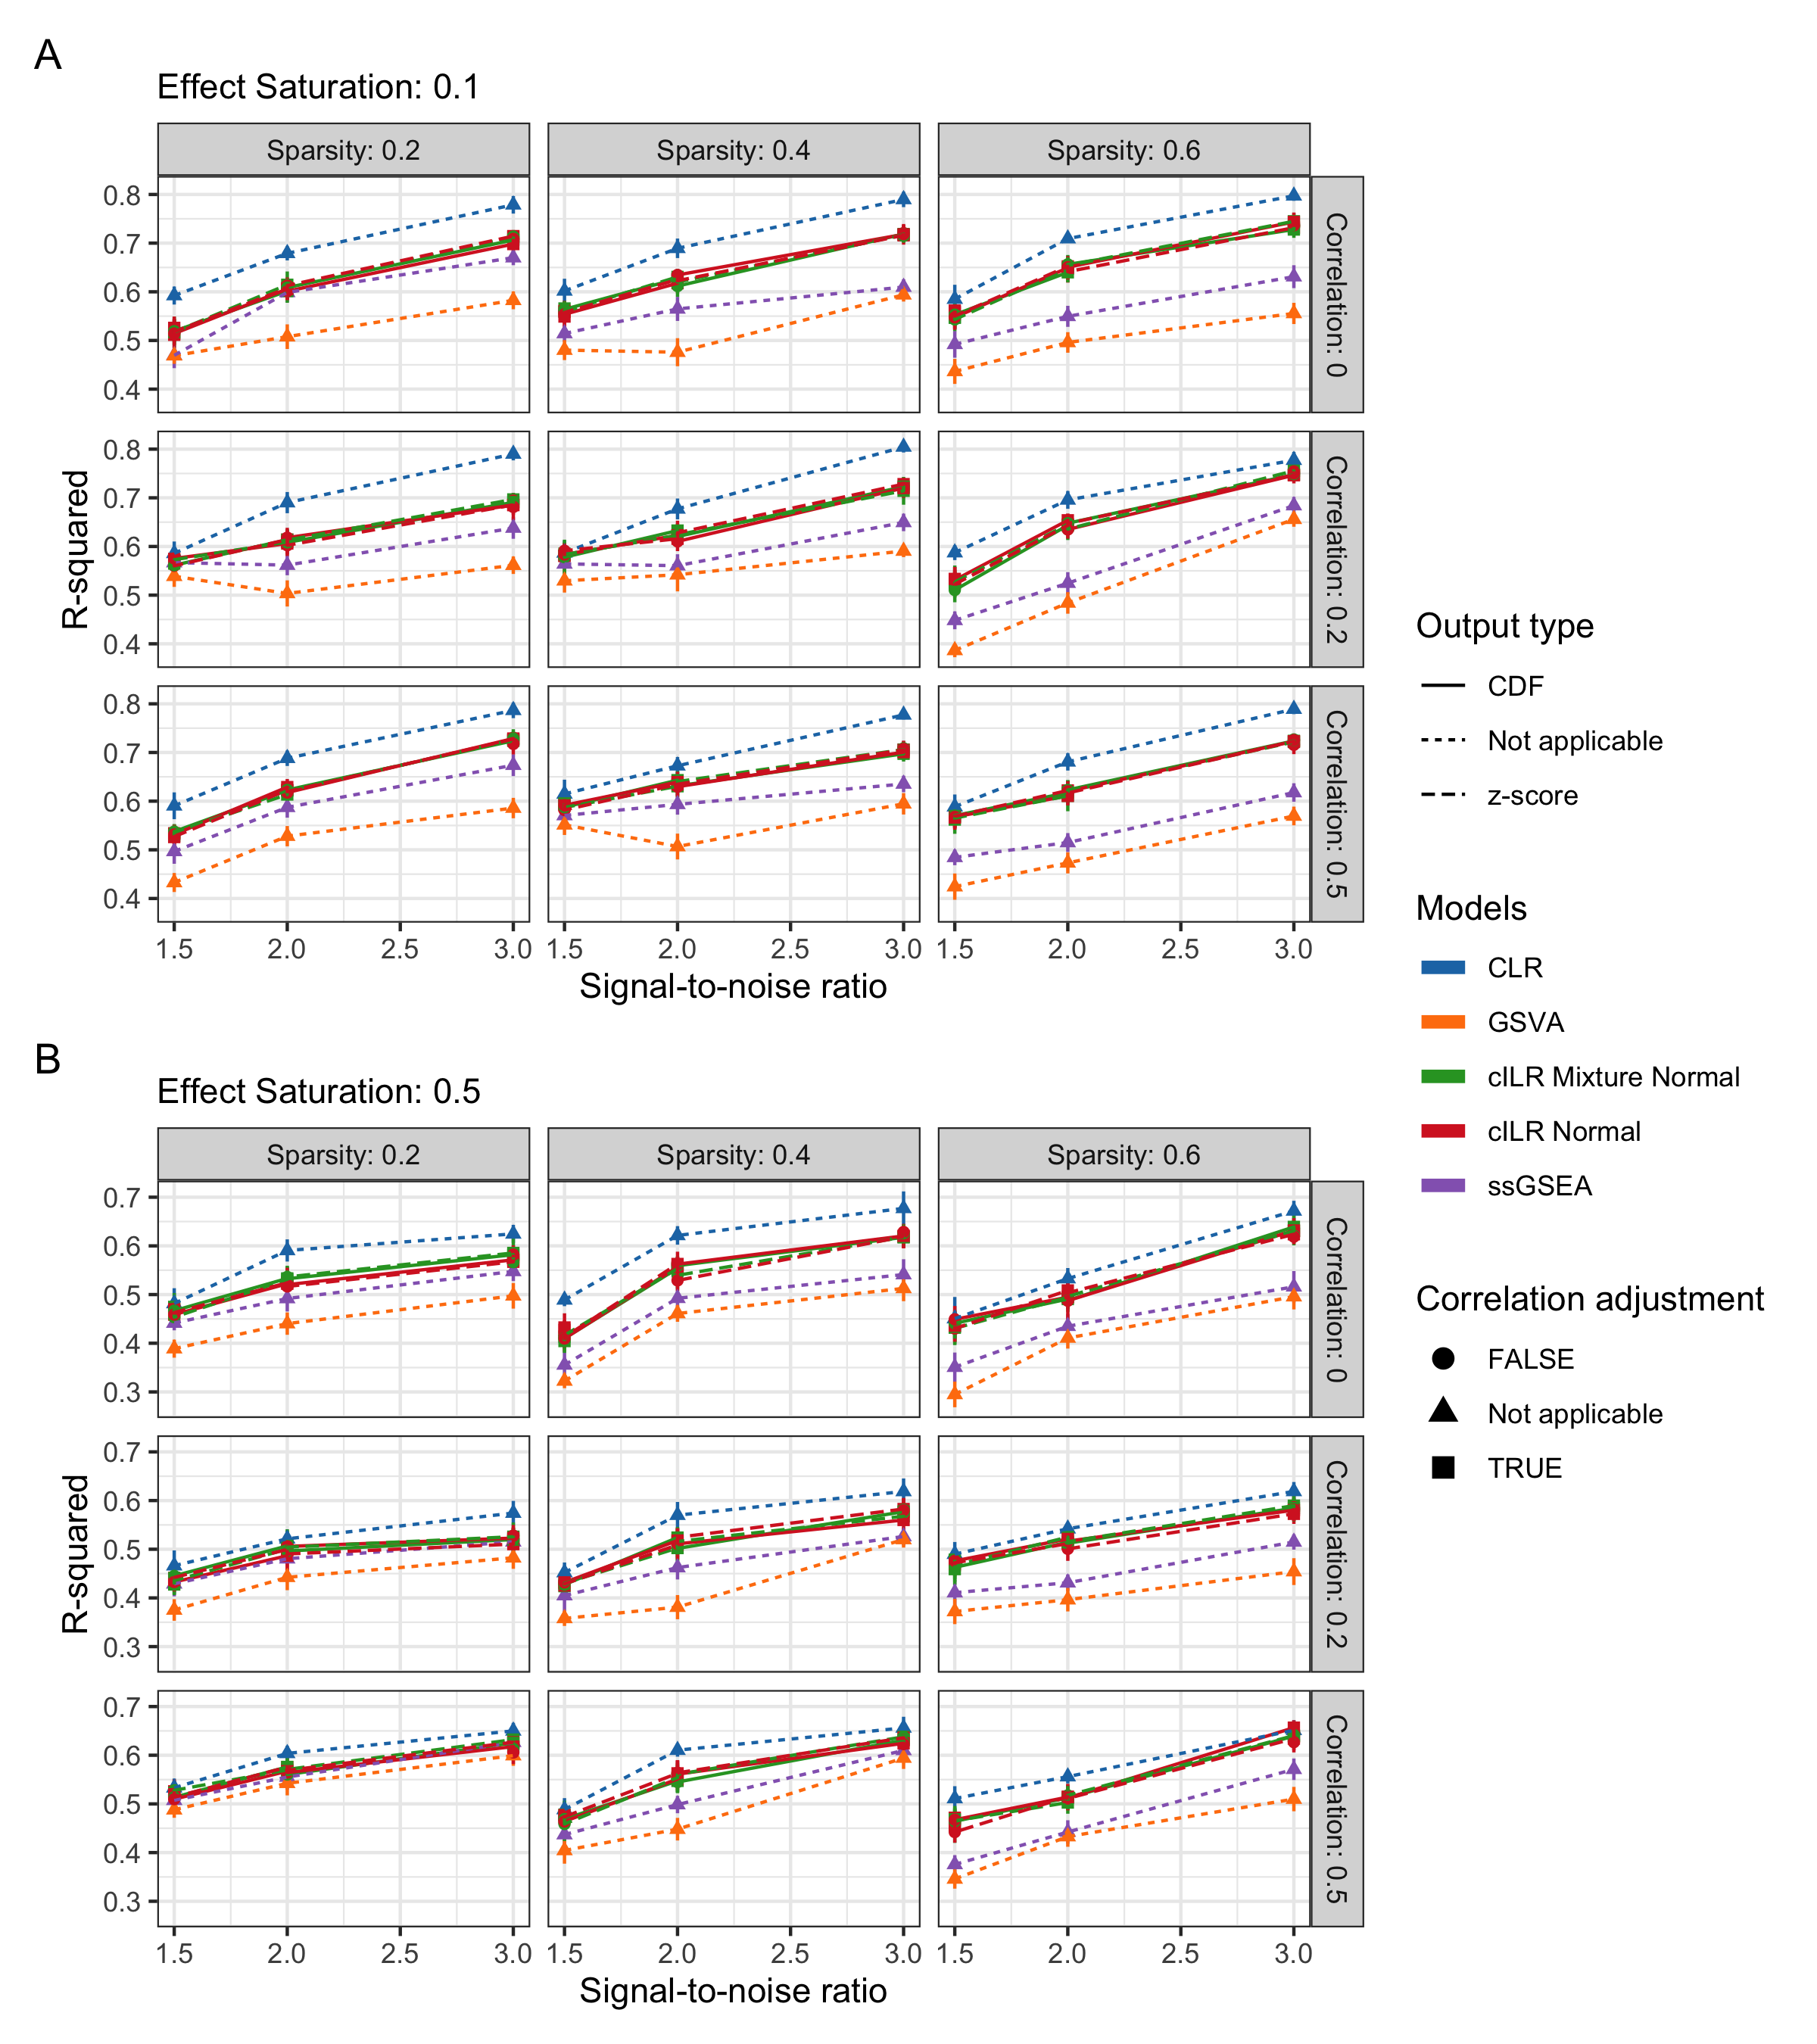
\includegraphics[width=\textwidth]{figures/sim_pred_rsq.png}
%DIF <     \caption{Predictive R-squared of a random forest model for a continuous outcome trained on cILR,     %ssGSEA, GSVA generated scores as well as on standard CLR transformed data evaluated on simulated data %across sparsity levels, correlation, and signal-to-noise ratio. Panel \textbf{(A)} and \textbf{(B)} %represent results across different levels of model saturation (proportion of sets associated with the %outcome). cILR approaches outperformed GSVA and ssGSEA but not standard CLR.}
%DIF >     \caption{Predictive R-squared of a random forest model for a continuous outcome trained on CBEA,     %ssGSEA, GSVA generated scores as well as on standard CLR transformed data evaluated on simulated data %across sparsity levels, correlation, and signal-to-noise ratio. Panel \textbf{(A)} and \textbf{(B)} %represent results across different levels of model saturation (proportion of sets associated with the %outcome). CBEA approaches outperformed GSVA and ssGSEA but not standard CLR.}
%    \label{fig:sim_pred_rsq}
%\end{figure}

\DIFdelbegin \subsubsection*{\DIFdel{Real data evaluations}}
%DIFAUXCMD
\DIFdel{In addition to parametric simulations, we also assessed the performance of using cILR scores in predictive models with real data sets. Fig~\ref{fig:7} presents results for }\DIFdelend \DIFaddbegin \DIFadd{We fit our model to }\DIFaddend two data sets with a similar disease classification task of discriminating patients who are diagnosed with IBD (includes both Crohn's disease and ulcerative colitis) using only microbiome taxonomic composition. The two data sets represent different microbiome sequencing aprpaoches: the Gevers et al. \cite{gevers2014} data set uses 16S rRNA gene sequencing, while the Nielsen et al \cite{nielsen2014} data set uses whole genome shotgun sequencing. 

\begin{figure}[!h]
    \centering
    \DIFdelbeginFL %DIFDELCMD < 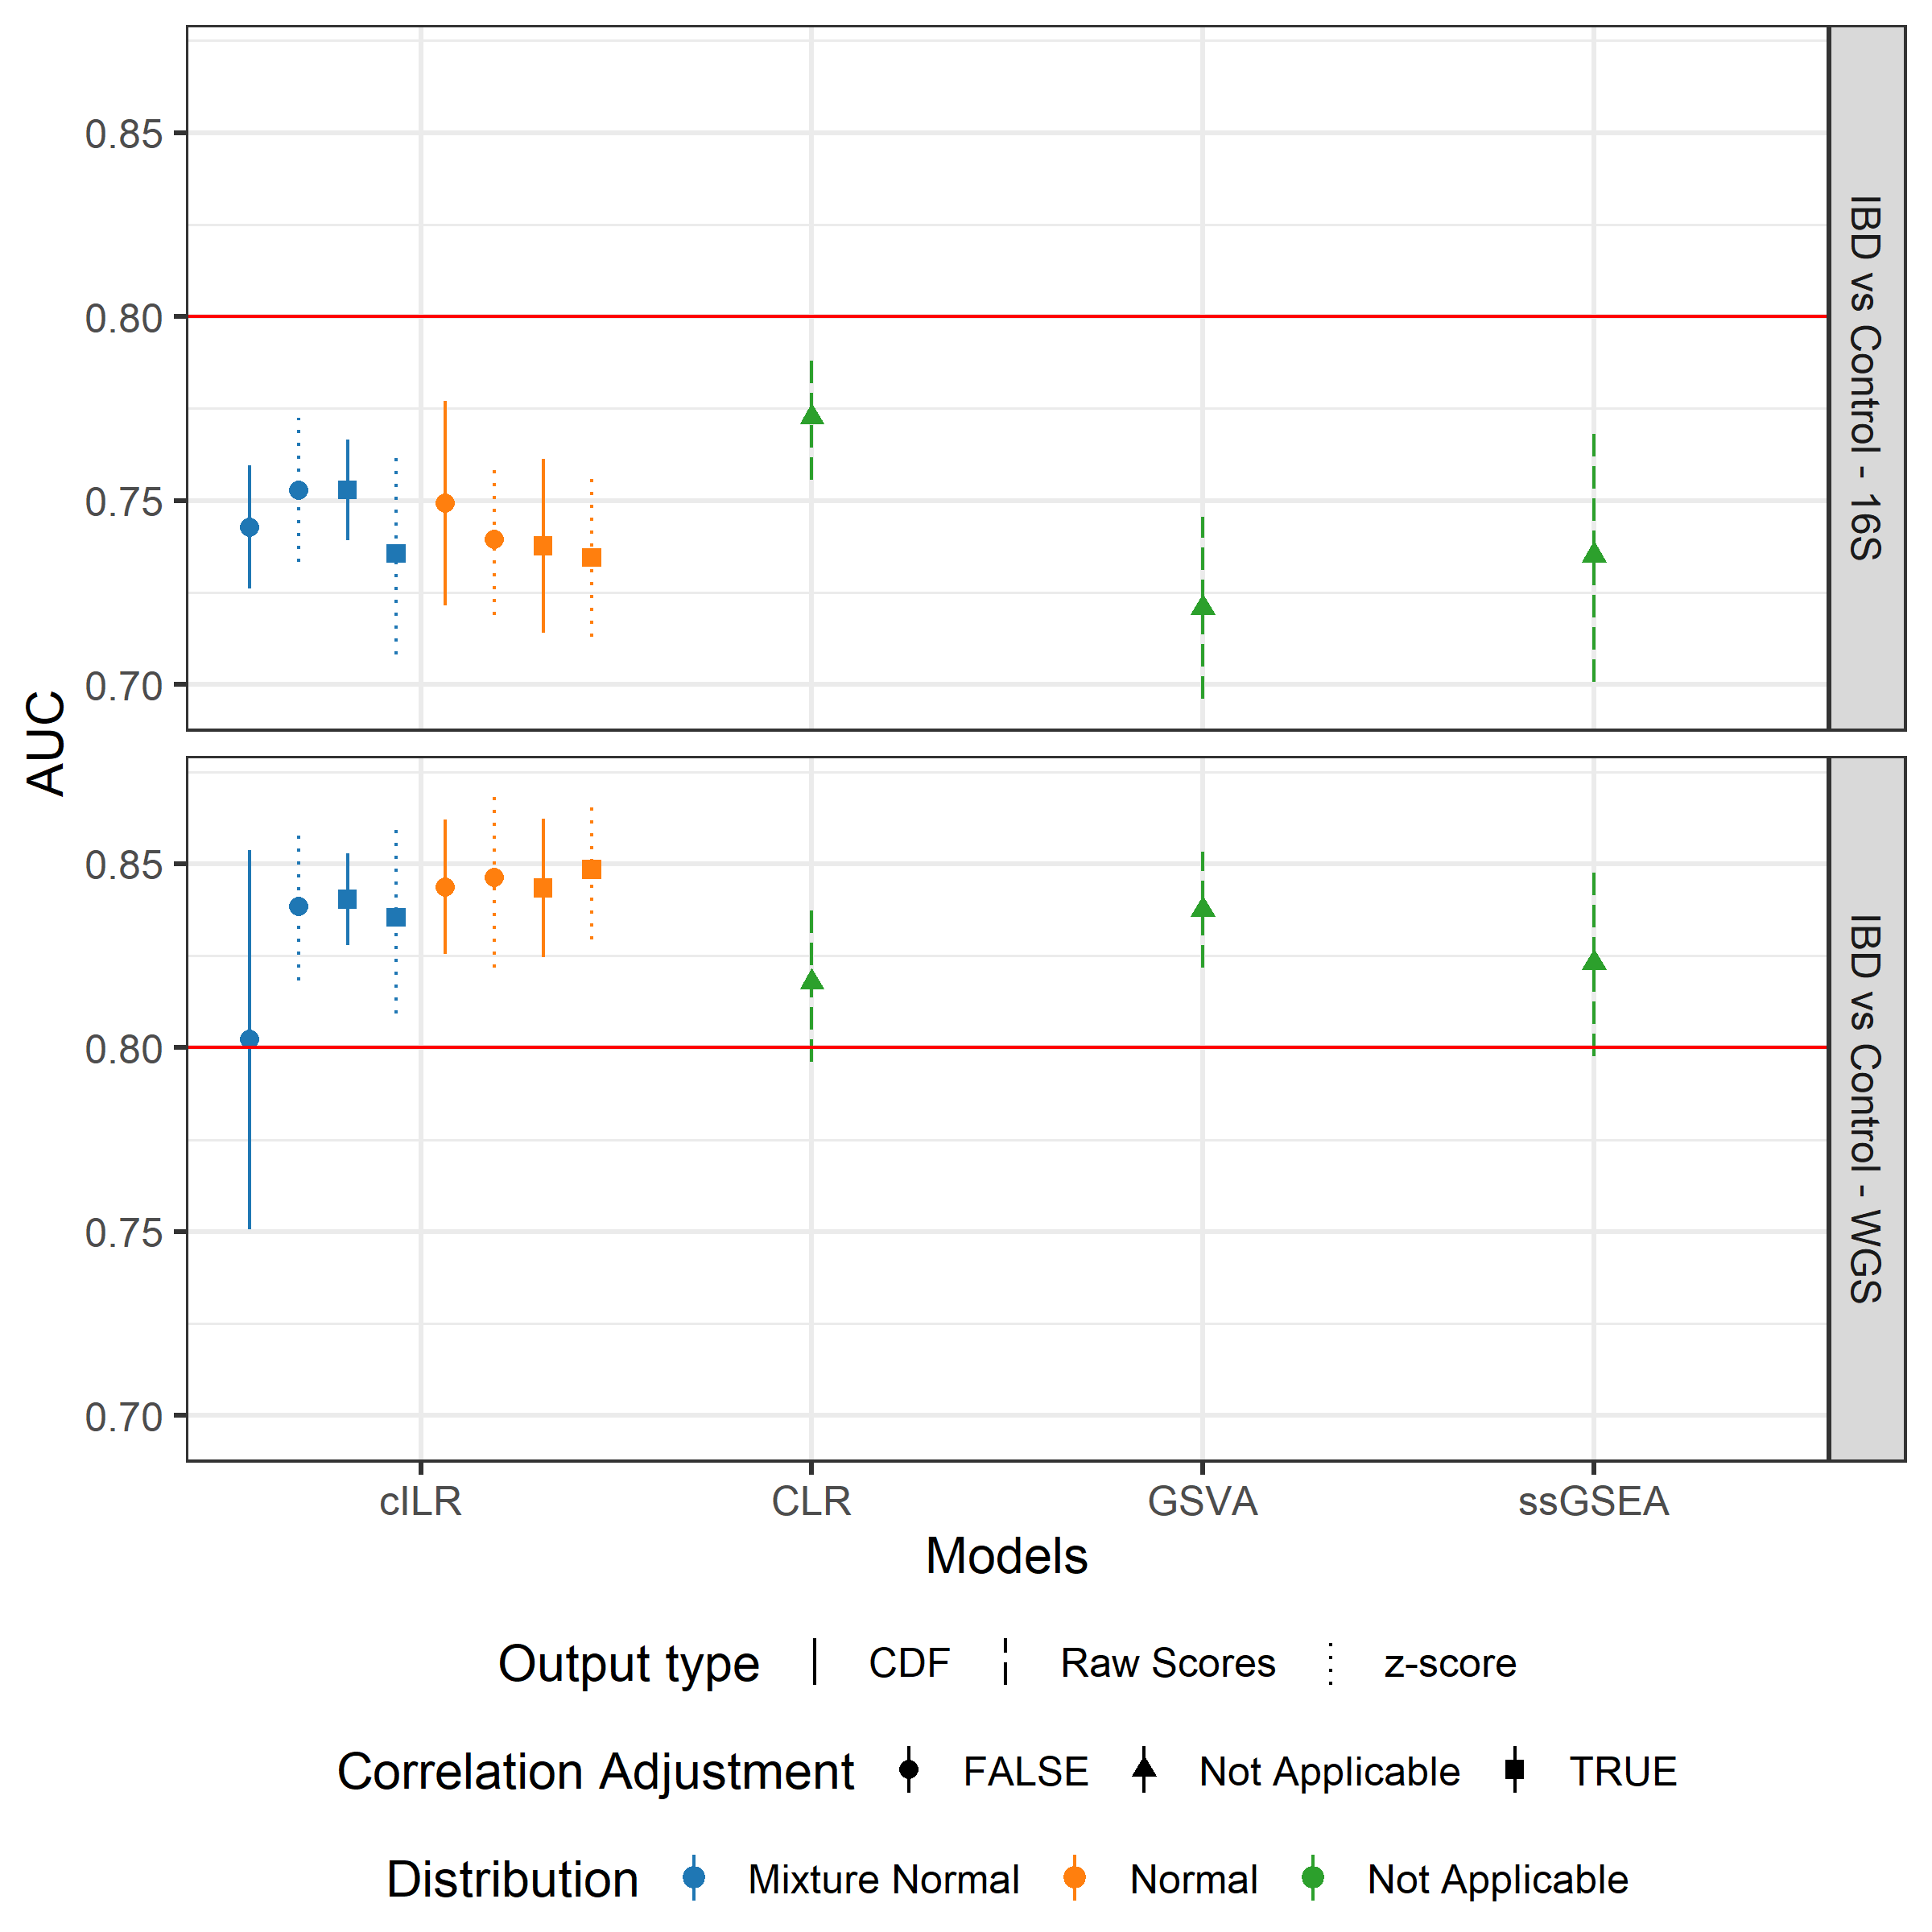
\includegraphics[width = \linewidth]{figures/data_prediction_plot.png}
%DIFDELCMD <     %%%
\DIFdelendFL \DIFaddbeginFL 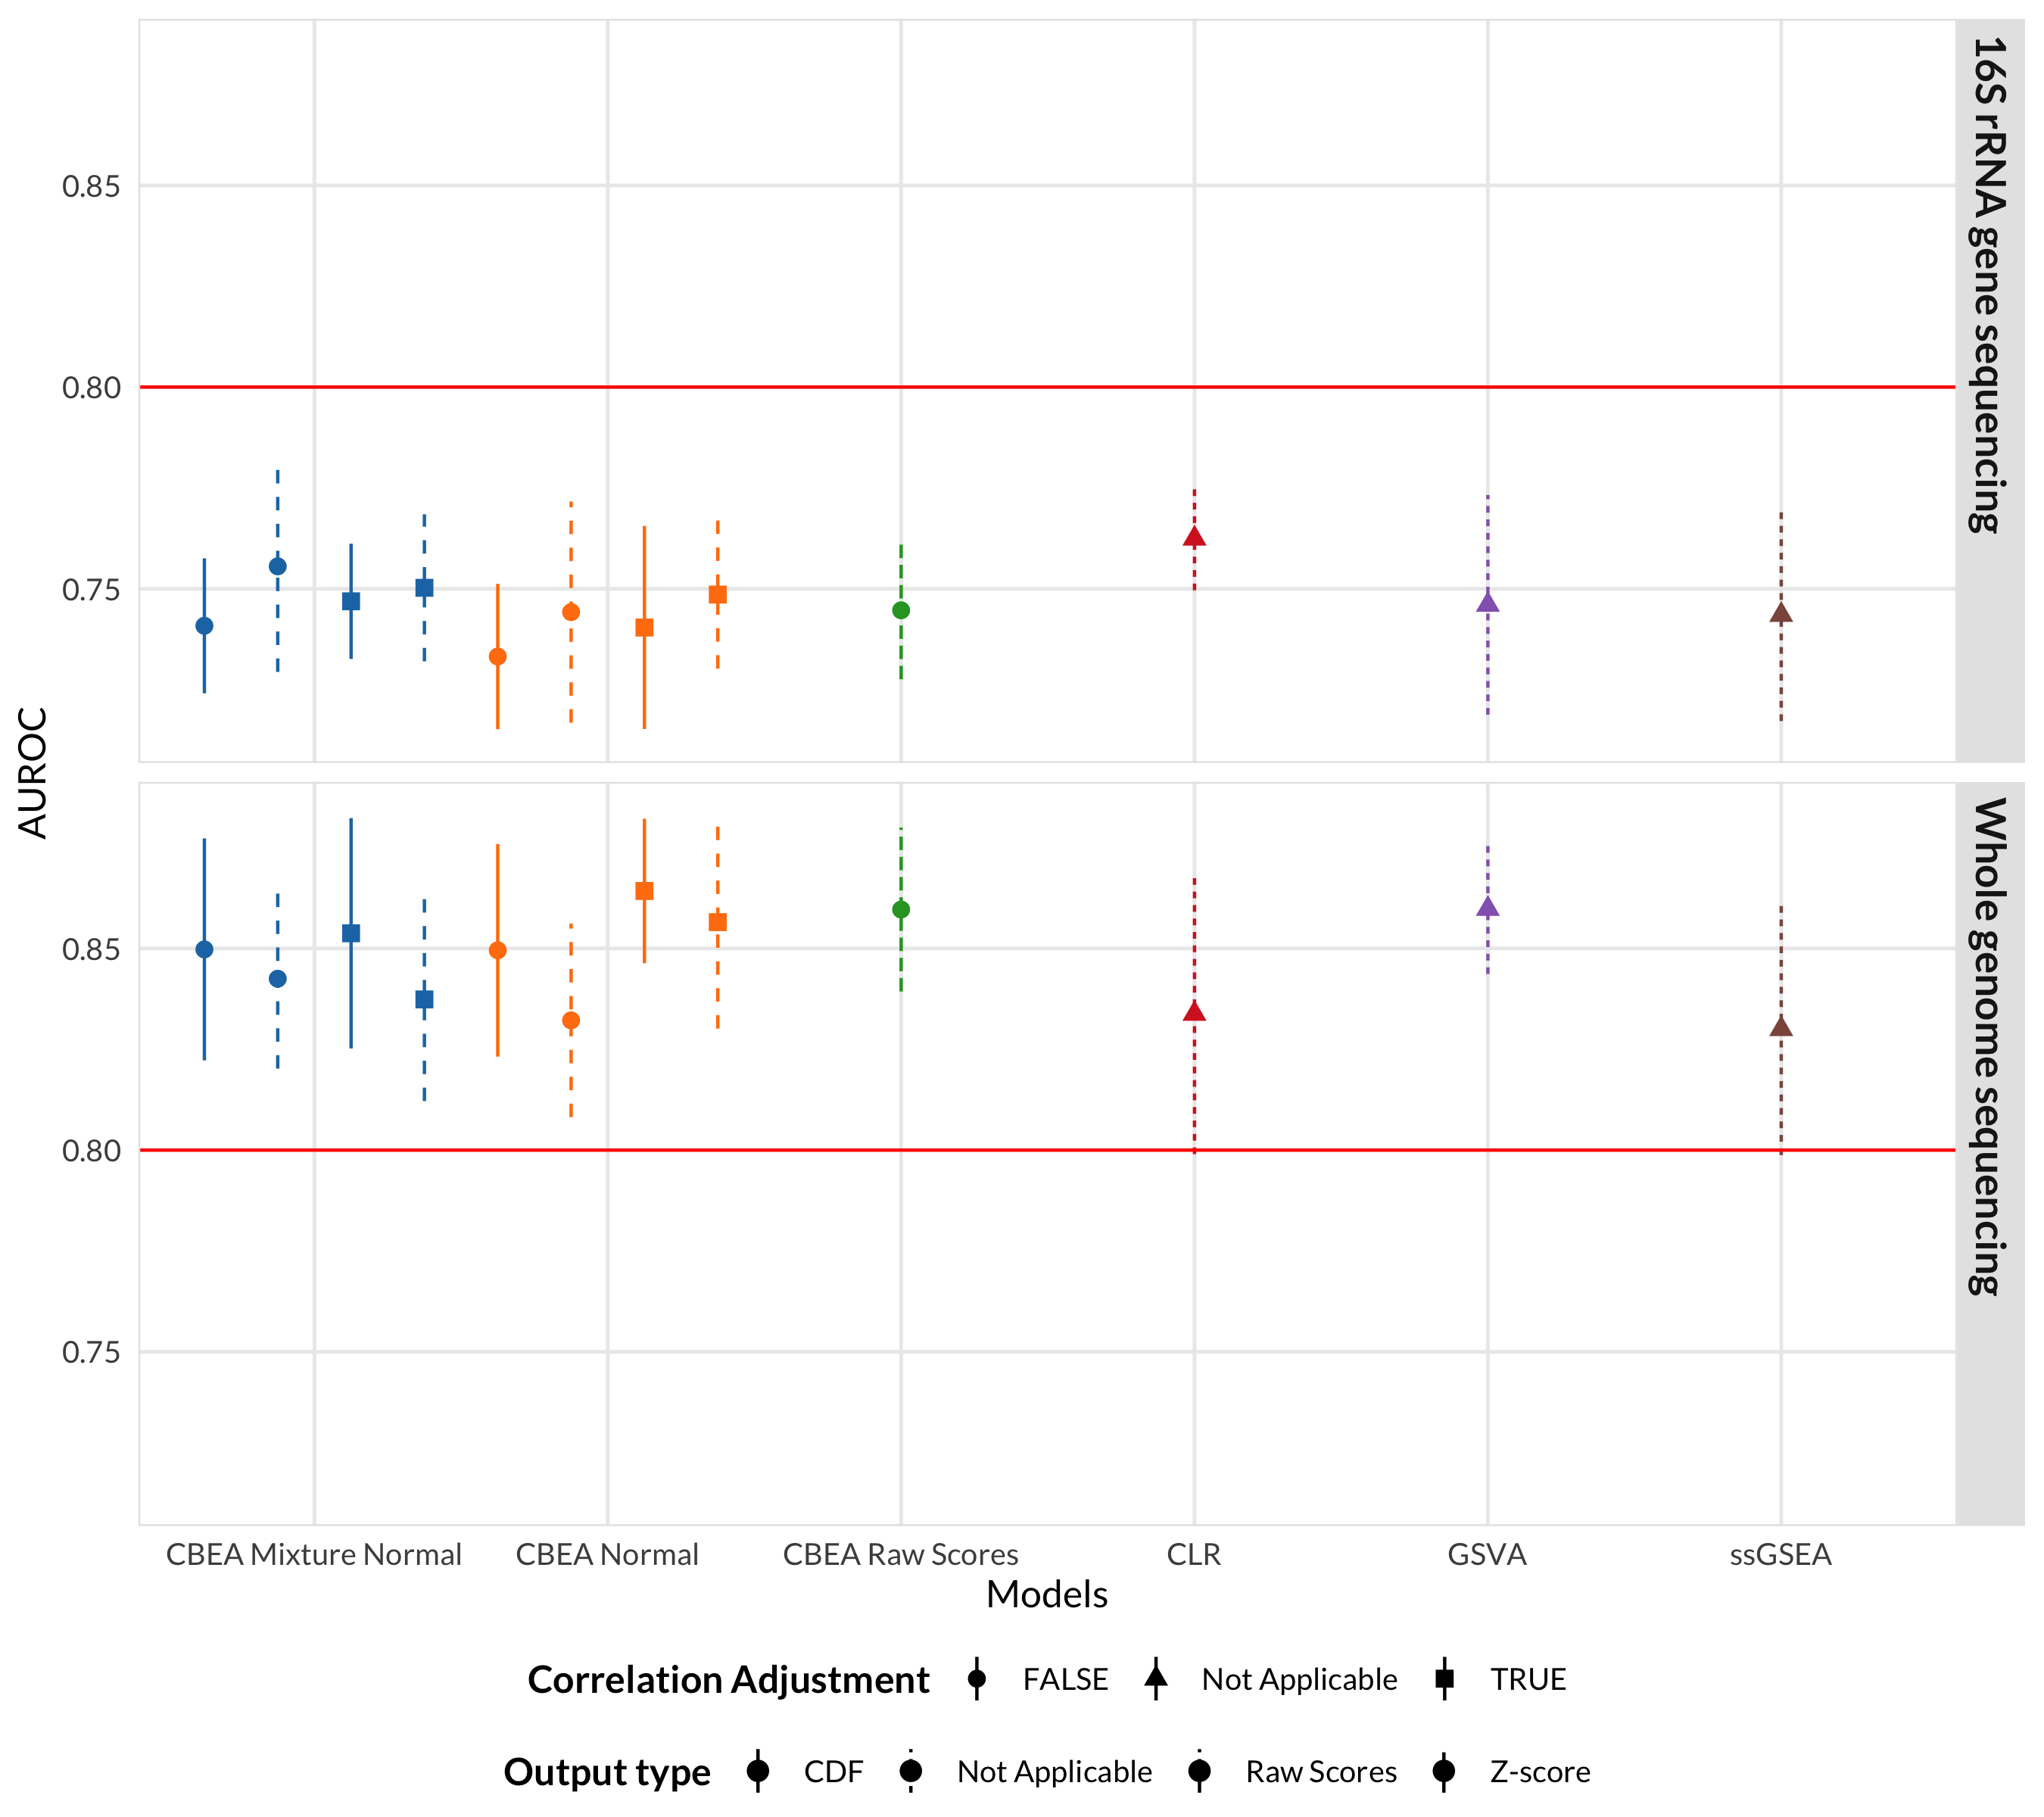
\includegraphics[width = \linewidth]{figures/data_pred.png}
    \DIFaddendFL \caption{Predictive performance of a naive random forest model trained on \DIFdelbeginFL \DIFdelFL{cILR}\DIFdelendFL \DIFaddbeginFL \DIFaddFL{CBEA}\DIFaddendFL , ssGSEA, GSVA generated scores as well as the standard CLR approach on predicting patients with inflammatory bowel disease versus controls using genus level taxonomic profiles. Data sets used span both 16S rRNA gene sequencing (Gevers et al. \cite{gevers2014}) and whole-genome shotgun sequencing (Nielsen et al. \cite{nielsen2014}). \DIFdelbeginFL \DIFdelFL{cILR }\DIFdelendFL \DIFaddbeginFL \DIFaddFL{CBEA }\DIFaddendFL performs better than GSVA and ssGSEA but not as well as CLR, with the exception of the whole genome sequencing data set.}
    \DIFdelbeginFL %DIFDELCMD < \label{fig:7}
%DIFDELCMD < %%%
\DIFdelendFL \DIFaddbeginFL \label{fig:6}
\DIFaddendFL \end{figure}

\DIFdelbegin \DIFdel{Similar to simulation experiments, we also fitted a naive random forest model using CILR, ssGSEA, GSVA, or CLR transformed variables as inputs, and use AUC as the performance criteria. Results also replicated that of the simulations, where across both data sets cILR and CLR methods provide much better performance than both GSVA or ssGSEA }\DIFdelend \DIFaddbegin \DIFadd{Fig~\ref{fig:6} illustrates the performance of our model with AUROC as the evaluation criteria. In the 16S rRNA data set, the best performing CBEA variant (CDF values computed from an unadjusted mixture normal distribution) outperforms both GSVA and ssGSEA but not the standard CLR approach}\DIFaddend . Interestingly, \DIFdelbegin \DIFdel{the cILR approach performed better than CLR }\DIFdelend in the whole genome \DIFdelbegin \DIFdel{data set but did not perform as well in the 16S rRNA gene sequencing data set}\DIFdelend \DIFaddbegin \DIFadd{sequencing data set, CBEA outperforms CLR, but were more similar in performance to GSVA}\DIFaddend . However, \DIFdelbegin \DIFdel{these results indicate that cILR }\DIFdelend \DIFaddbegin \DIFadd{due to large confidence intervals, no method were significantly out-performing other approaches evaluated. As such, these results indicated that CBEA }\DIFaddend generated scores are \DIFaddbegin \DIFadd{can be }\DIFaddend informative, providing competitive performance when acting as inputs to disease predictive models. \DIFdelbegin \DIFdel{Most importantly, performance values are consistent across both simulated and real data sets. 
}%DIFDELCMD < 

%DIFDELCMD < %%%
\DIFdel{These results demonstrate that cILR generated scores are informative features in disease prediction tasks. Simulation results indicate that cILR methods perform much better than either GSVA or ssGSEA, but not as well as the standard CLR approach}\DIFdelend \DIFaddbegin \DIFadd{Simulation studies (}\nameref{S5_Fig}\DIFadd{) showed similar results, however CBEA was more consistently underperforming compared to CLR across all scenarios}\DIFaddend . Interestingly, \DIFdelbegin \DIFdel{however, cILR methods were much more competitive with CLR in either WGS data sets or data sets with higher }\DIFdelend \DIFaddbegin \DIFadd{the performance gap decreases with increasing }\DIFaddend sparsity levels. 

\section*{Discussion}

\subsection*{Inference with \DIFdelbegin \DIFdel{cILR}\DIFdelend \DIFaddbegin \DIFadd{CBEA}\DIFaddend } 
\DIFaddbegin \DIFadd{CBEA is a microbiome-specific approach to generate sample specific enrichment scores for taxonomic sets defined apriori. }\DIFaddend The formulation of \DIFdelbegin \DIFdel{cILR }\DIFdelend \DIFaddbegin \DIFadd{CBEA }\DIFaddend as a comparison between taxa within the set and its complement corresponds to the competitive null hypothesis in the gene set testing literature \cite{tian2005}. \DIFdelbegin \DIFdel{This allows for conducting inference with cILR even at the sample-level. We assessed the usage of cILR in this type of analysis by evaluating type I error and power across both simulation studies and real data applications.  
Most importantly}\DIFdelend \DIFaddbegin \DIFadd{Since this null hypothesis is self-contained per sample, this allows users perform enrichment testing at the sample level. Additionally, in combination with a difference in means test, CBEA can also test for enrichment at the population level across case/control status similar to GSVA \mbox{%DIFAUXCMD
\cite{hanzelmann2013}}\hspace{0pt}%DIFAUXCMD
.  
}

\DIFadd{For single-sample analyses}\DIFaddend , we demonstrated that \DIFdelbegin \DIFdel{our adjusted cILR approach }\DIFdelend \DIFaddbegin \DIFadd{the CBEA approach (unadjusted with mixture normal parametric assumption) }\DIFaddend was able to \DIFdelbegin \DIFdel{address the issue of variance inflation due to correlation \mbox{%DIFAUXCMD
\cite{wu2012} }\hspace{0pt}%DIFAUXCMD
by controlling }\DIFdelend \DIFaddbegin \DIFadd{control }\DIFaddend for type I error at the \DIFdelbegin \DIFdel{appropriate $\alpha$ level across different levels of simulated inter-taxa correlation }\DIFdelend \DIFaddbegin \DIFadd{nominal level of 0.05 under the global null }\DIFaddend (Fig~\ref{fig:2}) while \DIFdelbegin \DIFdel{conversely unadjusted cILR and the naive Wilcoxon rank sum test showed much higher rates of error. This is further encouraged in real data analysis where the false discovery rate was around $0.05$ when a collection of true null and true alternate hypotheses were tested. Unfortunately the trade-off of good type I error control is lower power. The conservativeness of the test attenuates with higher sparsity and correlation, where power was not approaching even 50\% even at the highest effect sizes. However, when the degree of such data features are reasonable, cILR will still be able to detect a reasonable proportion of samples with inflated counts.  
}%DIFDELCMD < 

%DIFDELCMD < %%%
\DIFdel{We also observed that choosing different distributional forms did not alter performance values for cILR. This runs contrary to our comparison analysis in }\DIFdelend \DIFaddbegin \DIFadd{also demonstrating respectable power (Fig~\ref{fig:4}). This performance is consistent across different set sizes as well as our prior distributional fit analyses (}\DIFaddend Fig~\ref{fig:1}\DIFdelbegin \DIFdel{, where we demonstrated that }\DIFdelend \DIFaddbegin \DIFadd{), where }\DIFaddend the mixture normal \DIFdelbegin \DIFdel{distribution had superior fit compared to the simple normal for raw cILR scores computed under the global null . We hypothesized that this might be due to the difficulty in fitting mixture distributionto data using the expectation maximization algorithm, as the convergence rate is slow when there is high overlap between the mixtures, resulting in a small mixing coefficient for one of the components \mbox{%DIFAUXCMD
\cite{naim2012}}\hspace{0pt}%DIFAUXCMD
. As such, in our implementation of cILR, in order to ensure convergence for the estimating procedure we increased the number of iterations while relaxing the tolerance parameter. Furthermore, there are also possible problems with our adjustment procedure for the mixture distribution that might impact overall fit. In order to combine the scale and location estimate of two mixture distributions, we fixed the overall mean, standard deviation, mixing coefficient and component-wise means and used an optimization procedure to find the component-wise variances. However, this means that we have one equation for the overall variance but two possible parameters to estimate. As such, there is no guaranteed unique solution to component-wise variances. We hypothesized that the instability and degeneracy in component-wise variance estimates might impact the fidelity of estimates at the tails of the distribution, thereby affecting inference.  
}%DIFDELCMD < 

%DIFDELCMD < %%%
\DIFdel{Despite these concerns, empirical results still indicate that cILR can confidently identify samples with inflated counts. The conservativeness of the correlation adjustment procedure ensures that significant results can be trusted by practitioners, even if cILR might not be able to exhaustively identify all samples with inflated counts. In situations where either the data is less sparse (e.g. containing a lot of core taxa that are prevalent across all samples), there is less inter-taxa correlation within the set (e.g. taxa that do not participate in common pathways but have shared characteristics like pathogenicity), or if the effect size is large, then cILR will still be able to produce reasonable power. A practitioner can use cILR to screen for samples for subsequent analysis that might involve significant costs, or perform hypothesis generation using a less stringent criteria alongside a multiple testing adjustment procedure (such as Benjamini-Hochberg \mbox{%DIFAUXCMD
\cite{benjamini1995}}\hspace{0pt}%DIFAUXCMD
). 
}%DIFDELCMD < 

%DIFDELCMD < %%%
\subsection*{\DIFdel{Downstream analysis}}
%DIFAUXCMD
\DIFdel{The sample-level enrichment scores generated by the cILR method can be used in downstream analyses commonly performed in microbiome research: differential abundance testing and disease prediction}\DIFdelend \DIFaddbegin \DIFadd{displayed superior fit to the null distribution. Unfortunately, other variants of CBEA demonstrated neither good type I error control nor power. Interestingly, while the adjusted methods showed poor performance in real data evaluations (Fig~\ref{fig:2}), in simulation studies (}\nameref{S1_Fig}\DIFadd{, }\nameref{S3_Fig}\DIFadd{) these approaches were able to control for type I error well with the trade-off of much lower power}\DIFaddend .  

\DIFdelbegin \subsubsection*{\DIFdel{Differential abundance analysis}}
%DIFAUXCMD
\DIFdel{For differential abundance testing, we evaluated whether using cILR scores alongside a standard difference in means test (}\DIFdelend \DIFaddbegin \DIFadd{For population-level inference task, CBEA also performed very well. Under the permutation global null, representing genera abundance using CBEA scores in combination with }\DIFaddend Welch's t-test \DIFdelbegin \DIFdel{and Wilcoxon rank sum test ) is suitable to detect changes in abundance of a set of microbes. We compared cILR against two popular approaches: }\DIFdelend \DIFaddbegin \DIFadd{controls for type I error the correct $\alpha$ threshold while also keeping respectable power. Since population level enrichment test is equivalent to differential abundance using set-based features, we compared CBEA approach against using element-wise summations with }\DIFaddend corncob \cite{martin2020} and DESeq2 \cite{love2014} \DIFdelbegin \DIFdel{applied on data where taxa were aggregated using the naive sum method}\DIFdelend \DIFaddbegin \DIFadd{to test for set-level differential abundance}\DIFaddend . We chose DESeq2 because it is an older approach from the bulk RNA-seq literature that has strong support for usage in microbiome taxonomic data \cite{mcmurdie2014}. \DIFdelbegin \DIFdel{Conversely}\DIFdelend \DIFaddbegin \DIFadd{Alternately}\DIFaddend , corncob is a newer method developed specifically for microbiome taxonomic data sets, where taxonomic counts are modeled directly using a beta-binomial distribution instead of relying on normalization via size factor estimation\DIFdelbegin \DIFdel{like in DESeq2. }%DIFDELCMD < 

%DIFDELCMD < %%%
\DIFdel{Surprisingly, we found some conflicting results when evaluating comparisons across parametric simulations and real data analysis. The performance of cILR was consistent across two evaluation criteria, demonstrating good }\DIFdelend \DIFaddbegin \DIFadd{. We observed that using this approach resulted in an inflated }\DIFaddend type I error \DIFdelbegin \DIFdel{and respectable power . However, }\DIFdelend \DIFaddbegin \DIFadd{compared to all variants of CBEA (Fig~\ref{fig:2}), yet did not improve power (Fig~\ref{fig:4}). Results for CBEA approaches were replicated in simulation analyses, however for }\DIFaddend corncob and DESeq2 \DIFdelbegin \DIFdel{showed opposite effects}\DIFdelend \DIFaddbegin \DIFadd{we observed an opposite effect}\DIFaddend : in simulation experiments, both methods show good type I error control but low power \DIFdelbegin \DIFdel{, while in real data analyses, conversely both corncob and DESeq2 showed inflated type I error but comparable power with respect to cILR methods. Despite such discrepancy, results still indicate good performance of cILR scores when used as inputs to downstream differential abundance analysis compared to using aggregated raw counts, even in methods designed to handle that type of data such as corncob and DESeq2.
}\DIFdelend \DIFaddbegin \DIFadd{(}\nameref{S2_Fig}\DIFadd{, }\nameref{S4_Fig}\DIFadd{).  
}\DIFaddend 

\DIFdelbegin \DIFdel{We hypothesized that the above behavior can arise due to issues with performing inference in the presence }\DIFdelend \DIFaddbegin \DIFadd{We hypothesized that the discrepancy between simulation and real data evaluations can can arise due to differences in our assumptions regarding the data generating process that informed our simulation schema. For the non-zero component of each taxa, we sampled from the same negative binomial distribution where designated enriched taxa were generated with inflated means (but the same dispersion). These marginals were simulated to account for block exchangable correlation within the enriched set only. This might affect our results in two ways: First, our simulation scenario ensures that any designated non-enriched taxa is identical to each other. This is not the case for real data, where our null scenarios involves randomly sampled sets that might by chance all have taxa with inflated means compared to remainder taxa. This is represented in }\nameref{S7_Fig}\DIFadd{, where the distribution of type I error across our 500 replications are right skewed for underperforming CBEA variants, indicating that these approaches are much more sensitive compared to the Wilcoxon rank sum test or unadjusted CBEA with mixture normal distribution. Second, as described in the }\nameref{introduction} \DIFadd{section, we did not consider }\DIFaddend taxon-specific \DIFdelbegin \DIFdel{protocol biases \mbox{%DIFAUXCMD
\cite{mclaren2019}}\hspace{0pt}%DIFAUXCMD
. According to McLaren et al., }\DIFdelend \DIFaddbegin \DIFadd{biases that distort }\DIFaddend the observed relative abundance of taxa \DIFdelbegin \DIFdel{is different than the true relative abundance due to protocol bias, and importantly this bias is specific to each taxon \mbox{%DIFAUXCMD
\cite{mclaren2019}}\hspace{0pt}%DIFAUXCMD
. This is especially true in }\DIFdelend \DIFaddbegin \DIFadd{compred to true values \mbox{%DIFAUXCMD
\cite{mclaren2019}}\hspace{0pt}%DIFAUXCMD
. In }\DIFaddend the context of sum-based aggregations, \DIFdelbegin \DIFdel{where }\DIFdelend the resulting bias of the aggregated taxon are dependent on the relative abundances of the contributing taxa (Appendix I in \cite{mclaren2019}). Conceptually, this means that measurement error for a taxon aggregate is different across samples as relative abundance of contributing changes, leading to issues when attempting to perform inference. As such, we expect methods like corncob or DESeq2 when performed on such \DIFdelbegin \DIFdel{aggregates }\DIFdelend \DIFaddbegin \DIFadd{sum aggregates in the presence of taxon-specific biases }\DIFaddend to have inflated type I error compared to our taxon-ratio based approach. \DIFdelbegin %DIFDELCMD < 

%DIFDELCMD < %%%
\DIFdel{The bias model also helps explain differences in performance of DESeq2 and corncob in simulation analyses compared to real data. Our simulation protocol does not explicitly include bias in our formulation, and all taxa were generated from the same underlying distribution with similar variances across all samples (the only difference is in the mean value where a taxa is expected to have inflated counts). As such, we do not expect our simulated taxa to have any }\DIFdelend \DIFaddbegin \DIFadd{Conversely, in simulation studies, where }\DIFaddend taxon-specific biases \DIFdelbegin \DIFdel{, which is not the case in real data settings. Therefore, we can expect }\DIFdelend \DIFaddbegin \DIFadd{are absent, corncob and }\DIFaddend DESeq2 \DIFdelbegin \DIFdel{and corncob to retain their expected type I error control in simulation analyses compared to real data. It is still surprising to see lower power for both methods in simulation analyses, which might be due to the fact that the evaluation protocol only considers default settings for both methods and did not attempt to optimize performance}\DIFdelend \DIFaddbegin \DIFadd{should perform better}\DIFaddend . 

\DIFdelbegin \DIFdel{The fact that the performance of cILR remains consistent across both simulation and real data analysis shows that cILR is invariant to taxon-specific biases. Furthermore, our evaluation indicates that even a simple difference in means test when used in combination with cILR scores can preserve type I error while maintaining good power. As such , a practioner can use cILR as a pre-processing step prior to performing a differential abundance test. }\DIFdelend \DIFaddbegin \subsection*{\DIFadd{Downstream analysis using predictive models}}
\DIFadd{The sample-level enrichment scores generated by the CBEA method can be used in downstream analyses such as disease prediction. We evaluated whether CBEA can be used to generate set-based features for disease prediction models. 
}\DIFaddend 

\DIFdelbegin \subsubsection*{\DIFdel{Predictive models}}
%DIFAUXCMD
\DIFdel{For disease prediction , we }\DIFdelend \DIFaddbegin \DIFadd{We }\DIFaddend fitted a basic random forest model \cite{breiman2001} to predict continuous and binary outcomes using \DIFdelbegin \DIFdel{cILR }\DIFdelend \DIFaddbegin \DIFadd{CBEA }\DIFaddend generated scores as inputs. Similar to our inference analysis, we compared \DIFdelbegin \DIFdel{cILR }\DIFdelend \DIFaddbegin \DIFadd{CBEA }\DIFaddend against both ssGSEA and GSVA. Additionally, we also evaluated \DIFdelbegin \DIFdel{cILR }\DIFdelend \DIFaddbegin \DIFadd{CBEA }\DIFaddend with the approach where counts of a set were aggregated using sums and \DIFdelbegin \DIFdel{then }\DIFdelend \DIFaddbegin \DIFadd{applied the }\DIFaddend centered log-ratio \DIFdelbegin \DIFdel{transformed}\DIFdelend \DIFaddbegin \DIFadd{transformation (CLR)}\DIFaddend . This is because CLR is considered standard practice in using microbiome variables as predictors for a model \cite{gloor2017}. Results \DIFdelbegin \DIFdel{indicated that cILR produces good performance values }\DIFdelend \DIFaddbegin \DIFadd{showed that CBEA generate scores perform well }\DIFaddend across both real data \DIFdelbegin \DIFdel{analysis }\DIFdelend \DIFaddbegin \DIFadd{settings }\DIFaddend and simulation scenarios. Since predictive models consider the effect of variables jointly (and in the case of random forest, consider interactions as well), good performance indicates that \DIFdelbegin \DIFdel{cILR }\DIFdelend \DIFaddbegin \DIFadd{CBEA }\DIFaddend scores can capture joint distribution of sets, enabling both uniset and multi-set type analyses. Comparatively, \DIFdelbegin \DIFdel{cILR }\DIFdelend \DIFaddbegin \DIFadd{CBEA }\DIFaddend generated scores outperformed other enrichment score methods (GSVA and ssGSEA), suggesting that it is more tailored for microbiome taxonomic data sets. This is consistent with our sample ranking analysis (Fig~\DIFdelbegin \DIFdel{\ref{fig:3}}\DIFdelend \DIFaddbegin \DIFadd{\ref{fig:4}}\DIFaddend ), where \DIFdelbegin \DIFdel{cILR }\DIFdelend \DIFaddbegin \DIFadd{CBEA }\DIFaddend scores are on average more informative when used to rank samples based on their propensity to have inflated counts. However, \DIFdelbegin \DIFdel{cILR }\DIFdelend \DIFaddbegin \DIFadd{CBEA }\DIFaddend did not outperform the CLR approach across our simulation studies, and only marginally performed better in the real data analysis with WGS data. \DIFdelbegin %DIFDELCMD < 

%DIFDELCMD < %%%
\DIFdel{However}\DIFdelend \DIFaddbegin \DIFadd{Fortunately}\DIFaddend , in simulation studies, this performance gap between CLR and \DIFdelbegin \DIFdel{cILR }\DIFdelend \DIFaddbegin \DIFadd{CBEA }\DIFaddend decreases with higher sparsity and correlation, especially in low effect saturation scenarios.  
\DIFdelbegin \DIFdel{Additionally, there are also downsides to applying CLR. First, the singular covariance matrix of CLR transformed variables is singular due to a sum to zero constraint \mbox{%DIFAUXCMD
\cite{gloor2017}}\hspace{0pt}%DIFAUXCMD
, preventing the proper usage of approaches that rely on matrix decomposition. Second, the procedure still relies on using summation of counts prior to transformation, which means that we still can 't compare across sets of different sizes, and any bias might still be propagated \mbox{%DIFAUXCMD
\cite{mclaren2019}}\hspace{0pt}%DIFAUXCMD
. As such, despite benefits in performance for a naive random forest model, there is still space for using cILR as primary inputs into predictive models. }\DIFdelend 

\DIFdelbegin \DIFdel{Similar to other experiments in downstream usage of cILR, performance did not change with different underlying distributions, output types, or correlation status. This is surprising since we expect z-scores to perform better as they are able to capture the direction of an association. The fact that this effect persisted even onto our real data analysis suggests that this is not due to a deficiency of our simulation design.     
As such, practitioners who wish to use cILR in predictive models might be suited to use the settings that is the fastest to compute. }\DIFdelend \DIFaddbegin \subsection*{\DIFadd{Limitations and future directions}} 
\DIFaddend 

\DIFdelbegin \DIFdel{Ultimately, results indicate that cILR }\DIFdelend \DIFaddbegin \DIFadd{These above results demonstrate the applicability of CBEA under different data analysis scenarios. If researchers are interested in perform inference, they can decide between an unsupervised sample level approach (i.e. screen samples for enrichment of certain characteristics) or a supervised population level approach (i.e. identifying characteristics that are differentially abundant across case/control status). For the unsupervised approach, utilizing the unadjusted CBEA with the mixture normal distribution provides a good initial starting point. In the case where researchers only wants to screen samples with mean-inflated taxon sets (instead of additionally detecting taxon sets with increased correlation), they can apply the adjusted approach, which }\DIFaddend can \DIFaddbegin \DIFadd{be effective at conserving type I error even at high correlation scenarios. However, the trade off for this adjustment is power that decreases with increasing correlation. For the supervised analysis, all CBEA variants control well for type I error and provides adequate statistical power. However, using raw CBEA scores with difference-in-means test such as Welch's t-test is preferable since it requires the least amount of computing resource (no estimation process) while still outperforming using sum-based approach with a standard differential abundance test.     
}

\DIFadd{Beyond inference, CBEA scores are flexible and can be useful for downstream analysis. We demonstrated that for a given number of set-based features, CBEA can }\DIFaddend produce informative scores that contribute to competitive performance of prediction models even in low signal-to-noise ratios with high inter-taxa correlation and sparsity. \DIFdelbegin \DIFdel{Even though there exists situations where it might not provide maximum predictive values, the flexibility of cILR in various types of analyses enable even though in some scenarios it might not provide maximum predictive values}\DIFdelend \DIFaddbegin \DIFadd{This is especially true for whole genome sequencing data sets, where CBEA outperfrorms the standard approach of applying a CLR transformation. Researchers might find CBEA useful under situations of high sparsity and inter-taxa correlation, or if the property of a singular covariance matrix (a byproduct of the CLR transformation \mbox{%DIFAUXCMD
\cite{gloor2017}}\hspace{0pt}%DIFAUXCMD
) is undesired. Even though we only evaluated prediction models in this manuscript, researchers can benchmark their own usage of CBEA for other downstream tasks such as sample ordination}\DIFaddend . 

\DIFdelbegin \subsection*{\DIFdel{Limitations and future directions}} 
%DIFAUXCMD
\DIFdel{There }\DIFdelend \DIFaddbegin \DIFadd{However, there }\DIFaddend are various limitations to our evaluation of \DIFdelbegin \DIFdel{cILR}\DIFdelend \DIFaddbegin \DIFadd{CBEA}\DIFaddend . First, our simulation analysis might not capture the appropriate data-generating distributions underlying microbiome taxonomic data. There is strong evidence to suggest that our zero-inflated negative binomial distribution is representative \cite{calgaro2020}, however other distributions such as the Dirichlet multinomial distribution \DIFdelbegin \DIFdel{\mbox{%DIFAUXCMD
\cite{wu2016} }\hspace{0pt}%DIFAUXCMD
}\DIFdelend \DIFaddbegin \DIFadd{\mbox{%DIFAUXCMD
\cite{wu2016a} }\hspace{0pt}%DIFAUXCMD
}\DIFaddend have been used in the evaluation of prior studies. Second, \DIFaddbegin \DIFadd{we were not able to evaluate the phenotypical relevance of enrichment results as in Geistlinger et al. \mbox{%DIFAUXCMD
\cite{geistlinger2021} }\hspace{0pt}%DIFAUXCMD
due to limited consistent annotations for microbiome signatures in health and disease, especially those that are experimentally verified (and not just from differential abundance studies). We attempted to perform this evaluation by leveraging }\DIFaddend the \DIFdelbegin \DIFdel{usage of the }\DIFdelend gingival data set similar to \cite{calgaro2020}\DIFdelbegin \DIFdel{to assess power in differential abundance testing and single sample inference is not perfect. This is because the }\DIFdelend \DIFaddbegin \DIFadd{. However, we acknowledge that this is not a perfect solution, since }\DIFaddend oxygen usage label of each microbe in the data set is only available at the genus level, and the difference in counts for obligate aerobes and anaerobes across the supragingival and subgingival sites might not be as clear cut. As such, results from power analyses using this data set is only relative between the comparison methods \DIFaddbegin \DIFadd{instead of treated as absolute measures of power or phenotype relevance}\DIFaddend . Finally, we assumed that taxa within a set are all equally associated with the outcome. This limits our ability to evaluate the performance of \DIFdelbegin \DIFdel{cILR }\DIFdelend \DIFaddbegin \DIFadd{CBEA }\DIFaddend when only a small number of taxa within the set is associated with the outcome, or if there are variability in effect sizes or association direction of taxa within a set. 

Our evaluation \DIFaddbegin \DIFadd{also }\DIFaddend showed various drawbacks of the \DIFdelbegin \DIFdel{cILR method }\DIFdelend \DIFaddbegin \DIFadd{CBEA method itself}\DIFaddend . First, inference with \DIFdelbegin \DIFdel{cILR is limitedin being able to exhaustively detect all samples with significant inflated counts for a set in situations where there is a high degree of sparsity and }\DIFdelend \DIFaddbegin \DIFadd{CBEA at the sample level is limited, and can be affected by }\DIFaddend inter-taxa correlation \DIFaddbegin \DIFadd{if users wish to only detect mean-inflated sets}\DIFaddend . Second, for downstream analyses, \DIFdelbegin \DIFdel{cILR }\DIFdelend \DIFaddbegin \DIFadd{CBEA }\DIFaddend might not always perform better than competing methods, especially when being used to generate inputs to predictive models. We hypothesized that this might be due to the lack of fit for the underlying null distribution in high correlation settings, especially the identifiability problem associated \DIFaddbegin \DIFadd{the estimation procedure associated }\DIFaddend with adjusting the mixture normal distribution. As such, we hope to refine the null distribution estimating procedure by either choosing a better distributional form, or to further constrain the optimization procedure of the mixture normal distribution by fixing the third and fourth moments. 

In addition, \DIFdelbegin \DIFdel{there are possible extensions cILR can we can consider to provide more flexibility across different data analysis scenarios in data analysis. First, cILR did not address the sparsity of microbiome taxonomic dataand relies on }\DIFdelend \DIFaddbegin \DIFadd{CBEA itself did not consider other aspects of microbiome data. First, across all analyses, we relied on adding }\DIFaddend a pseudocount to ensure log operations are valid. \DIFdelbegin \DIFdel{We can address }\DIFdelend \DIFaddbegin \DIFadd{Users can directly addressing }\DIFaddend this by incorporating \DIFdelbegin \DIFdel{more sophisticated }\DIFdelend model-based \DIFdelbegin \DIFdel{zero-correction methods }\DIFdelend \DIFaddbegin \DIFadd{zero correction methods prior to modelling }\DIFaddend such as in \cite{martin-fernandez2012} or \cite{kaul2017a}. \DIFdelbegin \DIFdel{Second, cILR }\DIFdelend \DIFaddbegin \DIFadd{However, in our simulation studies, sparsity seems to not have a significant impact on the overall performance of our approach. Second, CBEA }\DIFaddend also treated all taxa within the set as equally contributing to the set. Incorporation of taxa-specific weights \DIFaddbegin \DIFadd{(similar to PhILR \mbox{%DIFAUXCMD
\cite{silverman2017}}\hspace{0pt}%DIFAUXCMD
) }\DIFaddend could reduce the influence of outliers, such as rare or highly invariant taxa. Finally, \DIFdelbegin \DIFdel{curating sets based on }\emph{\DIFdel{apriori}} %DIFAUXCMD
\DIFdelend \DIFaddbegin \DIFadd{even though for a given set of apriori annotations CBEA can generate useful summary scores, such values are limited in their utility if the annotation themselves are not meaningful. As such, curating and validating sets (similar to MSigDB \mbox{%DIFAUXCMD
\cite{subramanian2005}}\hspace{0pt}%DIFAUXCMD
) based on physiological or genomic }\DIFaddend characteristics of microbes \DIFaddbegin \DIFadd{\mbox{%DIFAUXCMD
\cite{weissman2021} }\hspace{0pt}%DIFAUXCMD
or their association with human disease (in beta BugSigDB }\url{https://bugsigdb.org/Main_Page}\DIFadd{) }\DIFaddend can allow for incorporating functional insights into microbiome-outcome analyses\DIFdelbegin \DIFdel{while also improving interpretability when compared to using taxonomic categories such as phylum or genus alone}\DIFdelend .  

\section*{Conclusion}
Gene set testing, or pathway analysis is an important tool in the analysis of high-dimensional genomics data sets. However, limited work has been done developing set based methods specifically for microbiome relative abundance data. We introduced a new microbiome-specific method to generate set-based enrichment scores at the sample level. We demonstrated that our method can control for type I error for significance testing at the sample level, while generated scores are also valid inputs in downstream analyses, including disease prediction and differential abundance.  

\section*{Acknowledgments}
The authors thank Becky Lebeaux, Modupe Coker, Erika Dade, Jie Zhou, and Weston Viles for insightful comments and suggestions that greatly improved the paper. 

\nolinenumbers
% Either type in your references using
% \begin{thebibliography}{}
% \bibitem{}
% Text
% \end{thebibliography}
%
% or
%
% Compile your BiBTeX database using our plos2015.bst
% style file and paste the contents of your .bbl file
% here. See http://journals.plos.org/plosone/s/latex for 
% step-by-step instructions.
% 

%DIF <  \bibliography{tax_agg}{}
\DIFdelbegin %DIFDELCMD < 

%DIFDELCMD < %%%
\DIFdelend %DIF > \bibliography{references}{}
\begin{thebibliography}{10}

\bibitem{proctor2019}
Proctor LM, Creasy HH, Fettweis JM, {Lloyd-Price} J, Mahurkar A, Zhou W, et~al.
\newblock The {{Integrative Human Microbiome Project}}.
\newblock Nature. 2019;569(7758):641--648.
\newblock doi:{10.1038/s41586-019-1238-8}.

\DIFdelbegin \bibitem{sharma2019}
\DIFdelend \DIFaddbegin \bibitem{sharma2019a}
\DIFaddend Sharma S, Tripathi P.
\newblock Gut Microbiome and Type 2 Diabetes: Where We Are and Where to Go?
\newblock The Journal of Nutritional Biochemistry. 2019;63:101--108.
\newblock doi:{10.1016/j.jnutbio.2018.10.003}.

\bibitem{aoun2020}
Aoun A, Darwish F, Hamod N.
\newblock The {{Influence}} of the {{Gut Microbiome}} on {{Obesity}} in
  {{Adults}} and the {{Role}} of {{Probiotics}}, {{Prebiotics}}, and
  {{Synbiotics}} for {{Weight Loss}}.
\newblock Preventive Nutrition and Food Science. 2020;25(2):113--123.
\newblock doi:{10.3746/pnf.2020.25.2.113}.

\bibitem{cho2012}
Cho I, Blaser MJ.
\newblock The Human Microbiome: At the Interface of Health and Disease.
\newblock Nature Reviews Genetics. 2012;13(4):260--270.
\newblock doi:{10.1038/nrg3182}.

\bibitem{callahan2016}
Callahan BJ, McMurdie PJ, Rosen MJ, Han AW, Johnson AJA, Holmes SP.
\newblock {{DADA2}}: {{\DIFdelbegin \DIFdel{High}\DIFdelend \DIFaddbegin \DIFadd{High-resolution}\DIFaddend }} \DIFdelbegin \DIFdel{-Resolution }\DIFdelend Sample Inference from {{Illumina}}
  Amplicon Data.
\newblock Nature Methods. 2016;13(7):581--583.
\newblock doi:{10.1038/nmeth.3869}.

\bibitem{truong2015}
Truong DT, Franzosa EA, Tickle TL, Scholz M, Weingart G, Pasolli E, et~al.
\newblock {{MetaPhlAn2}} for Enhanced Metagenomic Taxonomic Profiling.
\newblock Nature Methods. 2015;12(10):902--903.
\newblock doi:{10.1038/nmeth.3589}.

\DIFdelbegin \bibitem{li2019}
\DIFdelend \DIFaddbegin \bibitem{li2019a}
\DIFaddend Li H.
\newblock Statistical and {{Computational Methods}} in {{Microbiome}} and
  {{Metagenomics}}.
\newblock In: Handbook of {{Statistical Genomics}}. {John Wiley \& Sons, Ltd};
  2019. p. 977--550.

\bibitem{li2015}
Li H.
\newblock Microbiome, {{Metagenomics}}, and {{\DIFdelbegin \DIFdel{High}%DIFDELCMD < }}%%%
\DIFdel{-}%DIFDELCMD < {{%%%
\DIFdel{Dimensional
  }\DIFdelend \DIFaddbegin \DIFadd{High-Dimensional }\DIFaddend Compositional
  Data Analysis}}.
\newblock Annual Review of Statistics and Its Application. 2015;2(1):73--94.
\newblock doi:{10.1146/annurev-statistics-010814-020351}.

\DIFdelbegin \bibitem{shi2016}
\DIFdel{Shi P, Zhang A, Li H.
}%DIFDELCMD < \newblock %%%
\DIFdel{Regression Analysis for Microbiome Compositional Data.
}%DIFDELCMD < \newblock %%%
\DIFdel{The Annals of Applied Statistics. 2016;10(2):1019--1040.
}%DIFDELCMD < \newblock %%%
\DIFdel{doi:}%DIFDELCMD < {%%%
\DIFdel{10.1214/16-AOAS928}%DIFDELCMD < }%%%
\DIFdel{.
}%DIFDELCMD < 

%DIFDELCMD < \bibitem{sankaran2014}
\DIFdel{Sankaran K, Holmes S.
}%DIFDELCMD < \newblock {{%%%
\DIFdel{structSSI}%DIFDELCMD < }}%%%
\DIFdel{: }%DIFDELCMD < {{%%%
\DIFdel{Simultaneous}%DIFDELCMD < }} %%%
\DIFdel{and }%DIFDELCMD < {{%%%
\DIFdel{Selective Inference}%DIFDELCMD < }} %%%
\DIFdel{for
  }%DIFDELCMD < {{%%%
\DIFdel{Grouped}%DIFDELCMD < }} %%%
\DIFdel{or }%DIFDELCMD < {{%%%
\DIFdel{Hierarchically Structured Data}%DIFDELCMD < }}%%%
\DIFdel{.
}%DIFDELCMD < \newblock %%%
\DIFdel{Journal of statistical software. 2014;59(13):1--21.
}%DIFDELCMD < \newblock %%%
\DIFdel{doi:}%DIFDELCMD < {%%%
\DIFdel{10.18637/jss.v059.i13}%DIFDELCMD < }%%%
\DIFdel{.
}%DIFDELCMD < 

%DIFDELCMD < \bibitem{benjamini1995}
\DIFdel{Benjamini Y, Hochberg Y.
}%DIFDELCMD < \newblock %%%
\DIFdel{Controlling the }%DIFDELCMD < {{%%%
\DIFdel{False Discovery Rate}%DIFDELCMD < }}%%%
\DIFdel{: }%DIFDELCMD < {{%%%
\DIFdel{A Practical}%DIFDELCMD < }} %%%
\DIFdel{and
  }%DIFDELCMD < {{%%%
\DIFdel{Powerful Approach}%DIFDELCMD < }} %%%
\DIFdel{to }%DIFDELCMD < {{%%%
\DIFdel{Multiple Testing}%DIFDELCMD < }}%%%
\DIFdel{.
}%DIFDELCMD < \newblock %%%
\DIFdel{Journal of the Royal Statistical Society Series B (Methodological).
  1995;57(1):289--300.
}%DIFDELCMD < 

%DIFDELCMD < \bibitem{chen2018}
\DIFdel{Chen J, King E, Deek R, Wei Z, Yu Y, Grill D, et~al.
}%DIFDELCMD < \newblock %%%
\DIFdel{An Omnibus Test for Differential Distribution Analysis of Microbiome
  Sequencing Data.
}%DIFDELCMD < \newblock %%%
\DIFdel{Bioinformatics. 2018;34(4):643--651.
}%DIFDELCMD < \newblock %%%
\DIFdel{doi:}%DIFDELCMD < {%%%
\DIFdel{10.1093/bioinformatics/btx650}%DIFDELCMD < }%%%
\DIFdel{.
}%DIFDELCMD < 

%DIFDELCMD < \bibitem{weiss2017}
\DIFdel{Weiss S, Xu ZZ, Peddada S, Amir A, Bittinger K, Gonzalez A, et~al.
}%DIFDELCMD < \newblock %%%
\DIFdel{Normalization and Microbial Differential Abundance Strategies Depend
  upon Data Characteristics.
}%DIFDELCMD < \newblock %%%
\DIFdel{Microbiome. 2017;5(1).
}%DIFDELCMD < \newblock %%%
\DIFdel{doi:}%DIFDELCMD < {%%%
\DIFdel{10.1186/s40168-017-0237-y}%DIFDELCMD < }%%%
\DIFdel{.
}%DIFDELCMD < 

%DIFDELCMD < \bibitem{mcmurdie2014}
\DIFdel{McMurdie PJ, Holmes S.
}%DIFDELCMD < \newblock %%%
\DIFdel{Waste }%DIFDELCMD < {{%%%
\DIFdel{Not}%DIFDELCMD < }}%%%
\DIFdel{, }%DIFDELCMD < {{%%%
\DIFdel{Want Not}%DIFDELCMD < }}%%%
\DIFdel{: }%DIFDELCMD < {{%%%
\DIFdel{Why Rarefying Microbiome Data Is
  Inadmissible}%DIFDELCMD < }}%%%
\DIFdel{.
}%DIFDELCMD < \newblock %%%
\DIFdel{PLOS Computational Biology. 2014;10(4):e1003531.
}%DIFDELCMD < \newblock %%%
\DIFdel{doi:}%DIFDELCMD < {%%%
\DIFdel{10.1371/journal.pcbi.1003531}%DIFDELCMD < }%%%
\DIFdel{.
}%DIFDELCMD < 

%DIFDELCMD < \bibitem{love2014}
\DIFdel{Love MI, Huber W, Anders S.
}%DIFDELCMD < \newblock %%%
\DIFdel{Moderated Estimation of Fold Change and Dispersion for }%DIFDELCMD < {{%%%
\DIFdel{RNA}%DIFDELCMD < }}%%%
\DIFdel{-Seq
  Data with }%DIFDELCMD < {{%%%
\DIFdel{DESeq2}%DIFDELCMD < }}%%%
\DIFdel{.
}%DIFDELCMD < \newblock %%%
\DIFdel{Genome Biology. 2014;15(12):550.
}%DIFDELCMD < \newblock %%%
\DIFdel{doi:}%DIFDELCMD < {%%%
\DIFdel{10.1186/s13059-014-0550-8}%DIFDELCMD < }%%%
\DIFdel{.
}%DIFDELCMD < 

%DIFDELCMD < \bibitem{quinn2019}
\DIFdel{Quinn TP, Erb I, Gloor G, Notredame C, Richardson MF, Crowley TM.
}%DIFDELCMD < \newblock %%%
\DIFdel{A Field Guide for the Compositional Analysis of Any-Omics Data.
}%DIFDELCMD < \newblock %%%
\DIFdel{GigaScience. 2019;8(giz107).
}%DIFDELCMD < \newblock %%%
\DIFdel{doi:}%DIFDELCMD < {%%%
\DIFdel{10.1093/gigascience/giz107}%DIFDELCMD < }%%%
\DIFdel{.
}%DIFDELCMD < 

%DIFDELCMD < \bibitem{quinn2018b}
\DIFdel{Quinn TP, Erb I, Richardson MF, Crowley TM.
}%DIFDELCMD < \newblock %%%
\DIFdel{Understanding Sequencing Data as Compositions: An Outlook and Review.
}%DIFDELCMD < \newblock %%%
\DIFdel{Bioinformatics. 2018;34(16):2870--2878.
}%DIFDELCMD < \newblock %%%
\DIFdel{doi:}%DIFDELCMD < {%%%
\DIFdel{10.1093/bioinformatics/bty175}%DIFDELCMD < }%%%
\DIFdel{.
}%DIFDELCMD < 

%DIFDELCMD < %%%
\DIFdelend \bibitem{gloor2017}
Gloor GB, Macklaim JM, {Pawlowsky-Glahn} V, Egozcue JJ.
\newblock Microbiome {{Datasets Are Compositional}}: {{And This Is Not
  Optional}}.
\newblock Frontiers in Microbiology. 2017;8.
\newblock doi:{10.3389/fmicb.2017.02224}.

\DIFdelbegin \bibitem{aitchison1999}
\DIFdel{Aitchison J.
}%DIFDELCMD < \newblock %%%
\DIFdel{A }%DIFDELCMD < {{%%%
\DIFdel{Concise Guide}%DIFDELCMD < }} %%%
\DIFdel{to }%DIFDELCMD < {{%%%
\DIFdel{Compositional Data Analysis}%DIFDELCMD < }}%%%
\DIFdel{. 1999; p. 134.
}%DIFDELCMD < 

%DIFDELCMD < \bibitem{kurtz2015}
\DIFdel{Kurtz ZD, M}%DIFDELCMD < {%%%
\DIFdel{\"u}%DIFDELCMD < }%%%
\DIFdel{ller CL, Miraldi ER, Littman DR, Blaser MJ, Bonneau RA.
}%DIFDELCMD < \newblock %%%
\DIFdel{Sparse and }%DIFDELCMD < {{%%%
\DIFdel{Compositionally Robust Inference}%DIFDELCMD < }} %%%
\DIFdel{of }%DIFDELCMD < {{%%%
\DIFdel{Microbial
  Ecological Networks}%DIFDELCMD < }}%%%
\DIFdel{.
}%DIFDELCMD < \newblock %%%
\DIFdel{PLOS Computational Biology. 2015;11(5):e1004226.
}%DIFDELCMD < \newblock %%%
\DIFdel{doi:}%DIFDELCMD < {%%%
\DIFdel{10.1371/journal.pcbi.1004226}%DIFDELCMD < }%%%
\DIFdel{.
}%DIFDELCMD < 

%DIFDELCMD < \bibitem{kaul2017}
\DIFdel{Kaul A, Davidov O, Peddada SD.
}%DIFDELCMD < \newblock %%%
\DIFdel{Structural Zeros in High-Dimensional Data with Applications to
  Microbiome Studies.
}%DIFDELCMD < \newblock %%%
\DIFdel{Biostatistics. 2017;18(3):422--433.
}%DIFDELCMD < \newblock %%%
\DIFdel{doi:}%DIFDELCMD < {%%%
\DIFdel{10.1093/biostatistics/kxw053}%DIFDELCMD < }%%%
\DIFdel{.
}%DIFDELCMD < 

%DIFDELCMD < \bibitem{kaul2017a}
\DIFdel{Kaul A, Mandal S, Davidov O, Peddada SD.
}%DIFDELCMD < \newblock %%%
\DIFdel{Analysis of }%DIFDELCMD < {{%%%
\DIFdel{Microbiome Data}%DIFDELCMD < }} %%%
\DIFdel{in the }%DIFDELCMD < {{%%%
\DIFdel{Presence}%DIFDELCMD < }} %%%
\DIFdel{of }%DIFDELCMD < {{%%%
\DIFdel{Excess
  Zeros}%DIFDELCMD < }}%%%
\DIFdel{.
}%DIFDELCMD < \newblock %%%
\DIFdel{Frontiers in Microbiology. 2017;8.
}%DIFDELCMD < \newblock %%%
\DIFdel{doi:}%DIFDELCMD < {%%%
\DIFdel{10.3389/fmicb.2017.02114}%DIFDELCMD < }%%%
\DIFdel{.
}%DIFDELCMD < 

%DIFDELCMD < %%%
\DIFdelend \bibitem{khatri2012}
Khatri P, Sirota M, Butte AJ.
\newblock Ten {{Years}} of {{Pathway Analysis}}: {{Current Approaches}} and
  {{Outstanding Challenges}}.
\newblock PLOS Computational Biology. 2012;8(2):e1002375.
\newblock doi:{10.1371/journal.pcbi.1002375}.

\bibitem{goeman2007}
Goeman JJ, B{\"u}hlmann P.
\newblock Analyzing Gene Expression Data in Terms of Gene Sets: Methodological
  Issues.
\newblock Bioinformatics. 2007;23(8):980--987.
\newblock doi:{10.1093/bioinformatics/btm051}.

\bibitem{subramanian2005}
Subramanian A, Tamayo P, Mootha VK, Mukherjee S, Ebert BL, Gillette MA, et~al.
\newblock Gene Set Enrichment Analysis: {{A}} Knowledge-Based Approach for
  Interpreting Genome-Wide Expression Profiles.
\newblock Proceedings of the National Academy of Sciences.
  2005;102(43):15545--15550.
\newblock doi:{10.1073/pnas.0506580102}.

\bibitem{ashburner2000}
Ashburner M, Ball CA, Blake JA, Botstein D, Butler H, Cherry JM, et~al.
\newblock Gene {{Ontology}}: Tool for the Unification of Biology.
\newblock Nature genetics. 2000;25(1):25--29.
\newblock doi:{10.1038/75556}.

\DIFaddbegin \bibitem{irizarry2009}
\DIFadd{Irizarry RA, Wang C, Zhou Y, Speed TP.
}\newblock \DIFadd{Gene }{{\DIFadd{Set Enrichment Analysis Made Simple}}}\DIFadd{.
}\newblock \DIFadd{Statistical methods in medical research. 2009;18(6):565--575.
}\newblock \DIFadd{doi:}{\DIFadd{10.1177/0962280209351908}}\DIFadd{.
}

\DIFaddend \bibitem{hanzelmann2013}
H{\"a}nzelmann S, Castelo R, Guinney J.
\newblock {{GSVA}}: Gene Set Variation Analysis for Microarray and {{\DIFdelbegin \DIFdel{RNA}\DIFdelend \DIFaddbegin \DIFadd{RNA-Seq}\DIFaddend }}
  \DIFdelbegin \DIFdel{-}%DIFDELCMD < {{%%%
\DIFdel{Seq}%DIFDELCMD < }} %%%
\DIFdelend Data.
\newblock BMC Bioinformatics. 2013;14(1):7.
\newblock doi:{10.1186/1471-2105-14-7}.

\DIFdelbegin \bibitem{frost2020a}
\DIFdelend \DIFaddbegin \bibitem{frost2020}
\DIFaddend Frost HR.
\newblock Variance-Adjusted {{Mahalanobis}} ({{VAM}}): A Fast and Accurate
  Method for Cell-Specific Gene Set Scoring.
\newblock Nucleic Acids Research. 2020;48(16):e94--e94.
\newblock doi:{10.1093/nar/gkaa582}.

\DIFaddbegin \bibitem{chong2020}
\DIFadd{Chong J, Liu P, Zhou G, Xia J.
}\newblock \DIFadd{Using }{{\DIFadd{MicrobiomeAnalyst}}} \DIFadd{for Comprehensive Statistical,
  Functional, and Meta-Analysis of Microbiome Data.
}\newblock \DIFadd{Nature Protocols. 2020;15(3):799--821.
}\newblock \DIFadd{doi:}{\DIFadd{10.1038/s41596-019-0264-1}}\DIFadd{.
}

\bibitem{quinn2019}
\DIFadd{Quinn TP, Erb I, Gloor G, Notredame C, Richardson MF, Crowley TM.
}\newblock \DIFadd{A Field Guide for the Compositional Analysis of Any-Omics Data.
}\newblock \DIFadd{GigaScience. 2019;8(giz107).
}\newblock \DIFadd{doi:}{\DIFadd{10.1093/gigascience/giz107}}\DIFadd{.
}

\bibitem{quinn2018}
\DIFadd{Quinn TP, Erb I, Richardson MF, Crowley TM.
}\newblock \DIFadd{Understanding Sequencing Data as Compositions: An Outlook and Review.
}\newblock \DIFadd{Bioinformatics. 2018;34(16):2870--2878.
}\newblock \DIFadd{doi:}{\DIFadd{10.1093/bioinformatics/bty175}}\DIFadd{.
}

\bibitem{morton2019}
\DIFadd{Morton JT, Marotz C, Washburne A, Silverman J, Zaramela LS, Edlund A, et~al.
}\newblock \DIFadd{Establishing Microbial Composition Measurement Standards with
  Reference Frames.
}\newblock \DIFadd{Nature Communications. 2019;10(1).
}\newblock \DIFadd{doi:}{\DIFadd{10.1038/s41467-019-10656-5}}\DIFadd{.
}

\bibitem{love2014}
\DIFadd{Love MI, Huber W, Anders S.
}\newblock \DIFadd{Moderated Estimation of Fold Change and Dispersion for }{{\DIFadd{RNA-seq}}}
  \DIFadd{Data with }{{\DIFadd{DESeq2}}}\DIFadd{.
}\newblock \DIFadd{Genome Biology. 2014;15(12):550.
}\newblock \DIFadd{doi:}{\DIFadd{10.1186/s13059-014-0550-8}}\DIFadd{.
}

\bibitem{weiss2017}
\DIFadd{Weiss S, Xu ZZ, Peddada S, Amir A, Bittinger K, Gonzalez A, et~al.
}\newblock \DIFadd{Normalization and Microbial Differential Abundance Strategies Depend
  upon Data Characteristics.
}\newblock \DIFadd{Microbiome. 2017;5(1).
}\newblock \DIFadd{doi:}{\DIFadd{10.1186/s40168-017-0237-y}}\DIFadd{.
}

\bibitem{mcknight2019}
\DIFadd{McKnight DT, Huerlimann R, Bower DS, Schwarzkopf L, Alford RA, Zenger KR.
}\newblock \DIFadd{Methods for Normalizing Microbiome Data: }{{\DIFadd{An}}} \DIFadd{Ecological
  Perspective.
}\newblock \DIFadd{Methods in Ecology and Evolution. 2019;10(3):389--400.
}\newblock \DIFadd{doi:}{\DIFadd{10.1111/2041-210X.13115}}\DIFadd{.
}

\bibitem{aitchison1994}
\DIFadd{Aitchison J.
}\newblock \DIFadd{Principles of Compositional Data Analysis.
}\newblock \DIFadd{Lecture Notes-Monograph Series. 1994; p. 73--81.
}

\DIFaddend \bibitem{mclaren2019}
McLaren MR, Willis AD, Callahan BJ.
\newblock Consistent and Correctable Bias in Metagenomic Sequencing
  Experiments.
\newblock eLife. 2019;8:e46923.
\newblock doi:{10.7554/eLife.46923}.

\bibitem{egozcue2005}
Egozcue JJ, {Pawlowsky-Glahn} V.
\newblock Groups of {{Parts}} and {{Their Balances}} in {{Compositional Data
  Analysis}}.
\newblock Mathematical Geology. 2005;37(7):795--828.
\newblock doi:{10.1007/s11004-005-7381-9}.

\DIFdelbegin \bibitem{chong2020}
\DIFdel{Chong J, Liu P, Zhou G, Xia J.
}%DIFDELCMD < \newblock %%%
\DIFdel{Using }%DIFDELCMD < {{%%%
\DIFdel{MicrobiomeAnalyst}%DIFDELCMD < }} %%%
\DIFdel{for Comprehensive Statistical,
  Functional, and Meta-Analysis of Microbiome Data.
}%DIFDELCMD < \newblock %%%
\DIFdel{Nature Protocols. 2020;15(3):799--821.
}%DIFDELCMD < \newblock %%%
\DIFdel{doi:}%DIFDELCMD < {%%%
\DIFdel{10.1038/s41596-019-0264-1}%DIFDELCMD < }%%%
\DIFdel{.
}%DIFDELCMD < 

%DIFDELCMD < %%%
\DIFdelend \bibitem{tian2005}
Tian L, Greenberg SA, Kong SW, Altschuler J, Kohane IS, Park PJ.
\newblock Discovering Statistically Significant Pathways in Expression
  Profiling Studies.
\newblock Proceedings of the National Academy of Sciences.
  2005;102(38):13544--13549.
\newblock doi:{10.1073/pnas.0506577102}.

\DIFdelbegin \bibitem{egozcue2003}
\DIFdelend \DIFaddbegin \bibitem{rivera-pinto2018}
{\DIFadd{Rivera-Pinto}} \DIFadd{J, }\DIFaddend Egozcue JJ, {Pawlowsky-Glahn} V, \DIFdelbegin %DIFDELCMD < {%%%
\DIFdel{Mateu-Figueras}%DIFDELCMD < } %%%
\DIFdel{G}\DIFdelend \DIFaddbegin \DIFadd{Paredes R}\DIFaddend , {\DIFdelbegin \DIFdel{Barcelo-Vidal}\DIFdelend \DIFaddbegin \DIFadd{Noguera-Julian}\DIFaddend }
  \DIFdelbegin \DIFdel{C}\DIFdelend \DIFaddbegin \DIFadd{M, Calle ML}\DIFaddend .
\newblock \DIFdelbegin \DIFdel{Isometric }\DIFdelend \DIFaddbegin \DIFadd{Balances: A }\DIFaddend {{\DIFdelbegin \DIFdel{Logratio Transformations}\DIFdelend \DIFaddbegin \DIFadd{New Perspective}\DIFaddend }} for {{\DIFdelbegin \DIFdel{Compositional Data
  }\DIFdelend \DIFaddbegin \DIFadd{Microbiome }\DIFaddend Analysis}}.
\newblock \DIFdelbegin \DIFdel{Mathematical Geology. 2003;p.
~22.
}\DIFdelend \DIFaddbegin \DIFadd{mSystems. 2018;3(4):e00053--18.
}\newblock \DIFadd{doi:}{\DIFadd{10.1128/mSystems.00053-18}}\DIFadd{.
}\DIFaddend 

\DIFdelbegin \bibitem{silverman2017}
\DIFdel{Silverman JD, Washburne AD, Mukherjee S, David LA}\DIFdelend \DIFaddbegin \bibitem{wu2012}
\DIFadd{Wu D, Smyth GK}\DIFaddend .
\newblock \DIFdelbegin \DIFdel{A Phylogenetic Transform Enhances Analysis of Compositional
  Microbiota Data}\DIFdelend \DIFaddbegin \DIFadd{Camera: A Competitive Gene Set Test Accounting for Inter-Gene
  Correlation}\DIFaddend .
\newblock \DIFdelbegin \DIFdel{eLife. 2017;6:e21887}\DIFdelend \DIFaddbegin \DIFadd{Nucleic Acids Research. 2012;40(17):e133}\DIFaddend .
\newblock doi:{\DIFdelbegin \DIFdel{10.7554}\DIFdelend \DIFaddbegin \DIFadd{10.1093}\DIFaddend /\DIFdelbegin \DIFdel{eLife.21887}\DIFdelend \DIFaddbegin \DIFadd{nar/gks461}\DIFaddend }.

\DIFdelbegin \bibitem{barbie2009}
\DIFdel{Barbie DA, Tamayo P, Boehm JS, Kim SY, Moody SE, Dunn IF, et~al.
}%DIFDELCMD < \newblock %%%
\DIFdel{Systematic }\DIFdelend \DIFaddbegin \bibitem{egozcue2003}
\DIFadd{Egozcue JJ, }\DIFaddend {\DIFaddbegin \DIFadd{Pawlowsky-Glahn}} \DIFadd{V, }\DIFaddend {\DIFdelbegin \DIFdel{RNA}\DIFdelend \DIFaddbegin \DIFadd{Mateu-Figueras}\DIFaddend } \DIFdelbegin %DIFDELCMD < } %%%
\DIFdel{Interference Reveals That Oncogenic
  }\DIFdelend \DIFaddbegin \DIFadd{G, }\DIFaddend {\DIFaddbegin \DIFadd{Barcel}\DIFaddend {\DIFdelbegin %DIFDELCMD < {%%%
\emph{\DIFdel{KRAS}}%DIFAUXCMD
\DIFdelend \DIFaddbegin \DIFadd{\'o}\DIFaddend }\DIFaddbegin \DIFadd{-Vidal}\DIFaddend } \DIFaddbegin \DIFadd{C.
}\newblock \DIFadd{Isometric }{{\DIFadd{Logratio Transformations}\DIFaddend }\DIFdelbegin \DIFdel{-Driven Cancers Require }\DIFdelend \DIFaddbegin } \DIFadd{for }\DIFaddend {{\DIFdelbegin \DIFdel{TBK1}\DIFdelend \DIFaddbegin \DIFadd{Compositional Data
  Analysis}\DIFaddend }}.
\newblock \DIFdelbegin \DIFdel{Nature. 2009;462(7269):108--112}\DIFdelend \DIFaddbegin \DIFadd{Mathematical Geology. 2003;35(3):279--300}\DIFaddend .
\newblock doi:{\DIFdelbegin \DIFdel{10.1038}\DIFdelend \DIFaddbegin \DIFadd{10.1023}\DIFaddend /\DIFdelbegin \DIFdel{nature08460}\DIFdelend \DIFaddbegin \DIFadd{A:1023818214614}\DIFaddend }.

\bibitem{quast2013}
Quast C, Pruesse E, Yilmaz P, Gerken J, Schweer T, Yarza P, et~al.
\newblock The {{SILVA}} Ribosomal {{RNA}} Gene Database Project: Improved Data
  Processing and Web-Based Tools.
\newblock Nucleic Acids Research. 2013;41(D1):D590--D596.
\newblock doi:{10.1093/nar/gks1219}.

\bibitem{delignette-muller2015}
{Delignette-Muller} ML, Dutang C.
\newblock Fitdistrplus: {{An R}} Package for Fitting Distributions.
\newblock Journal of Statistical Software. 2015;64(4):1--34.

\bibitem{benaglia2009}
Benaglia T, Chauveau D, Hunter DR, Young D.
\newblock Mixtools: {{An R}} Package for Analyzing Finite Mixture Models.
\newblock Journal of Statistical Software. 2009;32(6):1--29.

\bibitem{washburne2017}
Washburne AD, Silverman JD, Leff JW, Bennett DJ, Darcy JL\DIFdelbegin \DIFdel{, Mukherjee S, et~al}\DIFdelend .
\newblock Phylogenetic Factorization of Compositional Data Yields Lineage-Level
  Associations in Microbiome Datasets.
\newblock PeerJ. 2017; \DIFdelbegin \DIFdel{5:e2969}\DIFdelend \DIFaddbegin \DIFadd{p.~26.
}

\bibitem{silverman2017}
\DIFadd{Silverman JD, Washburne AD, Mukherjee S, David LA.
}\newblock \DIFadd{A Phylogenetic Transform Enhances Analysis of Compositional
  Microbiota Data.
}\newblock \DIFadd{eLife. 2017;6:e21887}\DIFaddend .
\newblock doi:{\DIFdelbegin \DIFdel{10.7717}\DIFdelend \DIFaddbegin \DIFadd{10.7554}\DIFaddend /\DIFdelbegin \DIFdel{peerj.2969}\DIFdelend \DIFaddbegin \DIFadd{eLife.21887}\DIFaddend }.

\bibitem{morton2017}
Morton JT, Sanders J, Quinn RA, McDonald D, Gonzalez A, {V{\'a}zquez-Baeza} Y,
  et~al.
\newblock Balance {{Trees Reveal Microbial Niche Differentiation}}.
\newblock mSystems. 2017;2(1)\DIFaddbegin \DIFadd{:e00162--16}\DIFaddend .
\newblock doi:{10.1128/mSystems.00162-16}.

\DIFaddbegin \bibitem{aitchison1980}
\DIFadd{Aitchison J, Shen SM.
}\newblock \DIFadd{Logistic-Normal Distributions:}{{\DIFadd{Some}}} \DIFadd{Properties and Uses.
}\newblock \DIFadd{Biometrika. 1980;67(2):261--272.
}\newblock \DIFadd{doi:}{\DIFadd{10.1093/biomet/67.2.261}}\DIFadd{.
}

\DIFaddend \bibitem{efron2004}
Efron B.
\newblock Large-{{Scale Simultaneous Hypothesis Testing}}.
\newblock Journal of the American Statistical Association.
  2004;99(465):96--104.
\newblock doi:{10.1198/016214504000000089}.

\DIFdelbegin \bibitem{wu2012}
\DIFdel{Wu D, Smyth GK.
}%DIFDELCMD < \newblock %%%
\DIFdel{Camera: A Competitive Gene Set Test Accounting for Inter-Gene
  Correlation.
}%DIFDELCMD < \newblock %%%
\DIFdel{Nucleic Acids Research. 2012;40(17):e133.
}%DIFDELCMD < \newblock %%%
\DIFdel{doi:}\DIFdelend \DIFaddbegin \bibitem{kurtz2015a}
\DIFadd{Kurtz ZD, M}\DIFaddend {\DIFdelbegin \DIFdel{10.1093/nar/gks461}\DIFdelend \DIFaddbegin \DIFadd{\"u}\DIFaddend }\DIFaddbegin \DIFadd{ller CL, Miraldi ER, Littman DR, Blaser MJ, Bonneau RA}\DIFaddend .
\DIFdelbegin %DIFDELCMD < 

%DIFDELCMD < \bibitem{calgaro2020}
\DIFdel{Calgaro M, Romualdi C, Waldron L, Risso D, Vitulo N.
}\DIFdelend \newblock \DIFdelbegin \DIFdel{Assessment of Statistical Methods from Single Cell, Bulk }\DIFdelend \DIFaddbegin \DIFadd{Sparse and }\DIFaddend {{\DIFdelbegin \DIFdel{RNA}\DIFdelend \DIFaddbegin \DIFadd{Compositionally Robust Inference}\DIFaddend }} \DIFdelbegin \DIFdel{-Seq,
  and Metagenomics Applied to Microbiome Data.
}%DIFDELCMD < \newblock %%%
\DIFdel{Genome Biology. 2020;21(1):191.
}%DIFDELCMD < \newblock %%%
\DIFdel{doi:}%DIFDELCMD < {%%%
\DIFdel{10.1186/s13059-020-02104-1}%DIFDELCMD < }%%%
\DIFdel{.
}%DIFDELCMD < 

%DIFDELCMD < \bibitem{cario1997}
\DIFdel{Cario MC.
}%DIFDELCMD < \newblock %%%
\DIFdel{Modeling and }%DIFDELCMD < {{%%%
\DIFdel{Generating Random Vectors}%DIFDELCMD < }} %%%
\DIFdel{with }%DIFDELCMD < {{%%%
\DIFdel{Arbitrary Marginal
  Distributions}%DIFDELCMD < }} %%%
\DIFdel{and }%DIFDELCMD < {{%%%
\DIFdel{Correlation Matrix}%DIFDELCMD < }}%%%
\DIFdel{. 1997; p.~19.
}%DIFDELCMD < 

%DIFDELCMD < \bibitem{agresti1998}
\DIFdel{Agresti A, Coull BA.
}%DIFDELCMD < \newblock %%%
\DIFdel{Approximate }%DIFDELCMD < {{%%%
\DIFdel{Is Better}%DIFDELCMD < }} %%%
\DIFdel{than "}%DIFDELCMD < {{%%%
\DIFdel{Exact}%DIFDELCMD < }}%%%
\DIFdel{" for }%DIFDELCMD < {{%%%
\DIFdel{Interval
  Estimation}%DIFDELCMD < }} %%%
\DIFdelend of {{\DIFdelbegin \DIFdel{Binomial Proportions}\DIFdelend \DIFaddbegin \DIFadd{Microbial
  Ecological Networks}\DIFaddend }}.
\newblock \DIFdelbegin \DIFdel{The American Statistician. 1998;52(2):119--126}\DIFdelend \DIFaddbegin \DIFadd{PLOS Computational Biology. 2015;11(5):e1004226}\DIFaddend .
\newblock doi:{\DIFdelbegin \DIFdel{10.2307}\DIFdelend \DIFaddbegin \DIFadd{10.1371}\DIFaddend /\DIFdelbegin \DIFdel{2685469}%DIFDELCMD < }%%%
\DIFdel{.}%DIFDELCMD < 

%DIFDELCMD < \bibitem{delong1988}
\DIFdel{DeLong ER, DeLong DM, }%DIFDELCMD < {%%%
\DIFdel{Clarke-Pearson}\DIFdelend \DIFaddbegin \DIFadd{journal.pcbi.1004226}\DIFaddend }\DIFdelbegin \DIFdel{DL.
}%DIFDELCMD < \newblock %%%
\DIFdel{Comparing the Areas under Two or More Correlated Receiver Operating
  Characteristic Curves: A Nonparametric Approach.
}%DIFDELCMD < \newblock %%%
\DIFdel{Biometrics. 1988;44(3):837--845}\DIFdelend .

\DIFdelbegin \bibitem{hawinkel2019}
\DIFdel{Hawinkel S, Mattiello F, Bijnens L, Thas O}\DIFdelend \DIFaddbegin \bibitem{ackerman2009}
\DIFadd{Ackermann M, Strimmer K}\DIFaddend .
\newblock A \DIFdelbegin \DIFdel{Broken Promise: Microbiome Differential Abundance Methods Do Not
  Control the False Discovery Rate}\DIFdelend \DIFaddbegin \DIFadd{General Modular Framework for Gene Set Enrichment Analysis}\DIFaddend .
\newblock \DIFdelbegin \DIFdel{Briefings in Bioinformatics. 2019;20}\DIFdelend \DIFaddbegin \DIFadd{BMC bioinformatics. 2009;10}\DIFaddend (1):\DIFdelbegin \DIFdel{210--221.
}%DIFDELCMD < \newblock %%%
\DIFdel{doi:}%DIFDELCMD < {%%%
\DIFdel{10.1093/bib/bbx104}%DIFDELCMD < }%%%
\DIFdel{.
}\DIFdelend \DIFaddbegin \DIFadd{1--20.
}\DIFaddend 

\DIFdelbegin \bibitem{breiman2001}
\DIFdel{Breiman L}\DIFdelend \DIFaddbegin \bibitem{geistlinger2021}
\DIFadd{Geistlinger L, Csaba G, Santarelli M, Ramos M, Schiffer L, Turaga N, et~al}\DIFaddend .
\newblock \DIFdelbegin \DIFdel{Random }%DIFDELCMD < {{%%%
\DIFdel{Forests}%DIFDELCMD < }}%%%
\DIFdelend \DIFaddbegin \DIFadd{Toward a Gold Standard for Benchmarking Gene Set Enrichment Analysis}\DIFaddend .
\newblock \DIFdelbegin \DIFdel{Machine Learning. 2001;45(1):5--32.
}%DIFDELCMD < \newblock %%%
\DIFdel{doi:}%DIFDELCMD < {%%%
\DIFdel{10.1023/A:1010933404324}%DIFDELCMD < }%%%
\DIFdel{.
}\DIFdelend \DIFaddbegin \DIFadd{Briefings in bioinformatics. 2021;22(1):545--556.
}\DIFaddend 

\DIFdelbegin \bibitem{kuhn2020}
\DIFdel{Kuhn M, Wickham H.
}%DIFDELCMD < \newblock %%%
\DIFdel{Tidymodels: }%DIFDELCMD < {{%%%
\DIFdel{Easily}%DIFDELCMD < }} %%%
\DIFdel{Install and Load the 'tidymodels' Packages;
  2020.
}%DIFDELCMD < 

%DIFDELCMD < \bibitem{xiao2018}
\DIFdel{Xiao J, Chen L, Yu Y, Zhang X, Chen J.
}%DIFDELCMD < \newblock %%%
\DIFdel{A }%DIFDELCMD < {{%%%
\DIFdel{Phylogeny}%DIFDELCMD < }}%%%
\DIFdel{-}%DIFDELCMD < {{%%%
\DIFdel{Regularized Sparse Regression Model}%DIFDELCMD < }} %%%
\DIFdel{for
  }%DIFDELCMD < {{%%%
\DIFdel{Predictive Modeling}%DIFDELCMD < }} %%%
\DIFdel{of }%DIFDELCMD < {{%%%
\DIFdel{Microbial Community Data}%DIFDELCMD < }}%%%
\DIFdel{.
}%DIFDELCMD < \newblock %%%
\DIFdel{Frontiers in Microbiology. 2018;9.
}%DIFDELCMD < \newblock %%%
\DIFdel{doi:}%DIFDELCMD < {%%%
\DIFdel{10.3389/fmicb.2018.03112}%DIFDELCMD < }%%%
\DIFdel{.
}%DIFDELCMD < 

%DIFDELCMD < \bibitem{dong2020}
\DIFdel{Dong M, Li L, Chen M, Kusalik A, Xu W.
}%DIFDELCMD < \newblock %%%
\DIFdel{Predictive Analysis Methods for Human Microbiome Data with
  Application to }%DIFDELCMD < {{%%%
\DIFdel{Parkinson}%DIFDELCMD < }}%%%
\DIFdel{'s Disease.
}%DIFDELCMD < \newblock %%%
\DIFdel{PLOS ONE. 2020;15(8):e0237779.
}%DIFDELCMD < \newblock %%%
\DIFdel{doi:}%DIFDELCMD < {%%%
\DIFdel{10.1371/journal.pone.0237779}%DIFDELCMD < }%%%
\DIFdel{.
}%DIFDELCMD < 

%DIFDELCMD < %%%
\DIFdelend \bibitem{pasolli2017}
Pasolli E, Schiffer L, Manghi P, Renson A, Obenchain V, Truong DT, et~al.
\newblock Accessible, Curated Metagenomic Data through {{ExperimentHub}}.
\newblock Nature Methods. 2017;14(11):1023--1024.
\newblock doi:{10.1038/nmeth.4468}.

\bibitem{schiffer2019}
Schiffer L, Azhar R, Shepherd L, Ramos M, Geistlinger L, Huttenhower C, et~al.
\newblock {{HMP16SData}}: {{Efficient}} Access to the Human Microbiome Project
  through Bioconductor.
\newblock American Journal of Epidemiology. 2019;doi:{10.1093/aje/kwz006}.

\bibitem{gonzalez2018}
Gonzalez A, {Navas-Molina} JA, Kosciolek T, McDonald D, {V{\'a}zquez-Baeza} Y,
  Ackermann G, et~al.
\newblock Qiita: Rapid, Web-Enabled Microbiome Meta-Analysis.
\newblock Nature Methods. 2018;15(10):796--798.
\newblock doi:{10.1038/s41592-018-0141-9}.

\DIFaddbegin \bibitem{wickham2019}
\DIFadd{Wickham H, Averick M, Bryan J, Chang W, McGowan LD, Fran}{\DIFadd{\c c}}\DIFadd{ois R, et~al.
}\newblock \DIFadd{Welcome to the Tidyverse.
}\newblock \DIFadd{Journal of Open Source Software. 2019;4(43):1686.
}\newblock \DIFadd{doi:}{\DIFadd{10.21105/joss.01686}}\DIFadd{.
}

\bibitem{robin2011}
\DIFadd{Robin X, Turck N, Hainard A, Tiberti N, Lisacek F, Sanchez JC, et~al.
}\newblock {{\DIFadd{pROC}}}\DIFadd{: An Open-Source Package for }{{\DIFadd{R}}} \DIFadd{and }{{\DIFadd{S}}}\DIFadd{+ to Analyze and
  Compare }{{\DIFadd{ROC}}} \DIFadd{Curves.
}\newblock \DIFadd{BMC Bioinformatics. 2011;12:77.
}

\bibitem{mcmurdie2014}
\DIFadd{McMurdie PJ, Holmes S.
}\newblock \DIFadd{Waste }{{\DIFadd{Not}}}\DIFadd{, }{{\DIFadd{Want Not}}}\DIFadd{: }{{\DIFadd{Why Rarefying Microbiome Data Is
  Inadmissible}}}\DIFadd{.
}\newblock \DIFadd{PLOS Computational Biology. 2014;10(4):e1003531.
}\newblock \DIFadd{doi:}{\DIFadd{10.1371/journal.pcbi.1003531}}\DIFadd{.
}

\bibitem{ernst2021}
\DIFadd{Ernst FGM, Shetty SA, Borman T, Lahti L. Mia: }{{\DIFadd{Microbiome}}} \DIFadd{Analysis; 2021.
}

\bibitem{landau2021}
\DIFadd{Landau WM.
}\newblock \DIFadd{The Targets }{{\DIFadd{R}}} \DIFadd{Package: A Dynamic }{{\DIFadd{Make-like}}} \DIFadd{Function-Oriented
  Pipeline Toolkit for Reproducibility and High-Performance Computing.
}\newblock \DIFadd{Journal of Open Source Software. 2021;6(57):2959.
}

\DIFaddend \bibitem{consortium2012}
Consortium THMP, Huttenhower C, Gevers D, Knight R, Abubucker S, Badger JH,
  et~al.
\newblock Structure, Function and Diversity of the Healthy Human Microbiome.
\newblock Nature. 2012;486(7402):207--214.
\newblock doi:{10.1038/nature11234}.

\DIFaddbegin \bibitem{agresti1998}
\DIFadd{Agresti A, Coull BA.
}\newblock \DIFadd{Approximate }{{\DIFadd{Is Better}}} \DIFadd{than "}{{\DIFadd{Exact}}}\DIFadd{" for }{{\DIFadd{Interval
  Estimation}}} \DIFadd{of }{{\DIFadd{Binomial Proportions}}}\DIFadd{.
}\newblock \DIFadd{The American Statistician. 1998;52(2):119--126.
}\newblock \DIFadd{doi:}{\DIFadd{10.2307/2685469}}\DIFadd{.
}

\DIFaddend \bibitem{thurnheer2016}
Thurnheer T, Bostanci N, Belibasakis GN.
\newblock Microbial Dynamics during Conversion from Supragingival to
  Subgingival Biofilms in an in Vitro Model.
\newblock Molecular Oral Microbiology. 2016;31(2):125--135.
\newblock doi:{10.1111/omi.12108}.

\bibitem{beghini2019}
Beghini F, Renson A, Zolnik CP, Geistlinger L, Usyk M, Moody TU, et~al.
\newblock Tobacco Exposure Associated with Oral Microbiota Oxygen Utilization
  in the {{New York City Health}} and {{Nutrition Examination Study}}.
\newblock Annals of Epidemiology. 2019;34:18--25.e3.
\newblock doi:{10.1016/j.annepidem.2019.03.005}.

\bibitem{matteocalgaro2020}
Calgaro M. Mcalgaro93/Sc2meta: {{Paper Release}}; 2020.
\newblock Zenodo.

\DIFaddbegin \bibitem{delong1988}
\DIFadd{DeLong ER, DeLong DM, }{\DIFadd{Clarke-Pearson}} \DIFadd{DL.
}\newblock \DIFadd{Comparing the Areas under Two or More Correlated Receiver Operating
  Characteristic Curves: A Nonparametric Approach.
}\newblock \DIFadd{Biometrics. 1988;44(3):837--845.
}

\DIFaddend \bibitem{nielsen2014}
Nielsen HB, Almeida M, Juncker AS, Rasmussen S, Li J, Sunagawa S, et~al.
\newblock Identification and Assembly of Genomes and Genetic Elements in
  Complex Metagenomic Samples without Using Reference Genomes.
\newblock Nature Biotechnology. 2014;32(8):822--828.
\newblock doi:{10.1038/nbt.2939}.

\bibitem{gevers2014}
Gevers D, Kugathasan S, Denson LA, {V{\'a}zquez-Baeza} Y, Van~Treuren W, Ren B,
  et~al.
\newblock The {{\DIFdelbegin \DIFdel{Treatment}%DIFDELCMD < }}%%%
\DIFdel{-}%DIFDELCMD < {{%%%
\DIFdel{Naive }\DIFdelend \DIFaddbegin \DIFadd{Treatment-Naive }\DIFaddend Microbiome}} in {{\DIFdelbegin \DIFdel{New}%DIFDELCMD < }}%%%
\DIFdel{-}%DIFDELCMD < {{%%%
\DIFdel{Onset }\DIFdelend \DIFaddbegin \DIFadd{New-Onset }\DIFaddend Crohn}}'s
  {{Disease}}.
\newblock Cell Host \& Microbe. 2014;15(3):382--392.
\newblock doi:{10.1016/j.chom.2014.02.005}.

\DIFaddbegin \bibitem{breiman2001}
\DIFadd{Breiman L.
}\newblock \DIFadd{Random }{{\DIFadd{Forests}}}\DIFadd{.
}\newblock \DIFadd{Machine Learning. 2001;45(1):5--32.
}\newblock \DIFadd{doi:}{\DIFadd{10.1023/A:1010933404324}}\DIFadd{.
}

\bibitem{chawla2002}
\DIFadd{Chawla NV, Bowyer KW, Hall LO, Kegelmeyer WP.
}\newblock {{\DIFadd{SMOTE}}}\DIFadd{: }{{\DIFadd{Synthetic Minority Over-sampling Technique}}}\DIFadd{.
}\newblock \DIFadd{Journal of Artificial Intelligence Research. 2002;16:321--357.
}\newblock \DIFadd{doi:}{\DIFadd{10.1613/jair.953}}\DIFadd{.
}

\bibitem{kuhn2020}
\DIFadd{Kuhn M, Wickham H. Tidymodels: A Collection of Packages for Modeling and
  Machine Learning Using Tidyverse Principles.; 2020.
}

\DIFaddend \bibitem{martin2020}
Martin BD, Witten D, Willis AD.
\newblock Modeling Microbial Abundances and Dysbiosis with Beta-Binomial
  Regression.
\newblock The Annals of Applied Statistics. 2020;14(1):94--115.
\newblock doi:{10.1214/19-AOAS1283}.

\DIFdelbegin \bibitem{naim2012}
\DIFdel{Naim I, Gildea D}\DIFdelend \DIFaddbegin \bibitem{barbie2009}
\DIFadd{Barbie DA, Tamayo P, Boehm JS, Kim SY, Moody SE, Dunn IF, et~al}\DIFaddend .
\newblock \DIFdelbegin \DIFdel{Convergence of the }\DIFdelend \DIFaddbegin \DIFadd{Systematic }\DIFaddend {{\DIFdelbegin \DIFdel{EM Algorithm}\DIFdelend \DIFaddbegin \DIFadd{RNA}\DIFaddend }} \DIFdelbegin \DIFdel{for }\DIFdelend \DIFaddbegin \DIFadd{Interference Reveals That Oncogenic
  }\DIFaddend {{\DIFdelbegin \DIFdel{Gaussian Mixtures}\DIFdelend \DIFaddbegin {\emph{\DIFadd{KRAS}}\DIFaddend }}\DIFdelbegin \DIFdel{with
  }\DIFdelend \DIFaddbegin }\DIFadd{-Driven Cancers Require }\DIFaddend {{\DIFdelbegin \DIFdel{Unbalanced Mixing Coefficients}\DIFdelend \DIFaddbegin \DIFadd{TBK1}\DIFaddend }}.
\newblock \DIFdelbegin \DIFdel{Proceedings of the 29th International Coference on International
  Conference on Machine Learning. 2012;p.
~8.
}\DIFdelend \DIFaddbegin \DIFadd{Nature. 2009;462(7269):108--112.
}\DIFaddend \newblock doi:{\DIFdelbegin \DIFdel{10.5555}\DIFdelend \DIFaddbegin \DIFadd{10.1038}\DIFaddend /\DIFdelbegin \DIFdel{3042573.3042756}\DIFdelend \DIFaddbegin \DIFadd{nature08460}\DIFaddend }.

\DIFdelbegin \bibitem{wu2016}
\DIFdelend \DIFaddbegin \bibitem{calgaro2020}
\DIFadd{Calgaro M, Romualdi C, Waldron L, Risso D, Vitulo N.
}\newblock \DIFadd{Assessment of Statistical Methods from Single Cell, Bulk }{{\DIFadd{RNA-seq}}}\DIFadd{,
  and Metagenomics Applied to Microbiome Data.
}\newblock \DIFadd{Genome Biology. 2020;21(1):191.
}\newblock \DIFadd{doi:}{\DIFadd{10.1186/s13059-020-02104-1}}\DIFadd{.
}

\bibitem{wu2016a}
\DIFaddend Wu C, Chen J, Kim J, Pan W.
\newblock An Adaptive Association Test for Microbiome Data.
\newblock Genome Medicine. 2016;8(1):56.
\newblock doi:{10.1186/s13073-016-0302-3}.

\bibitem{martin-fernandez2012}
{Mart{\'i}n-Fern{\'a}ndez} JA, Hron K, Templ M, Filzmoser P,
  {Palarea-Albaladejo} J.
\newblock Model-Based Replacement of Rounded Zeros in Compositional Data:
  {{Classical}} and Robust Approaches.
\newblock Computational Statistics \& Data Analysis. 2012;56(9):2688--2704.
\newblock doi:{10.1016/j.csda.2012.02.012}.

\DIFaddbegin \bibitem{kaul2017a}
\DIFadd{Kaul A, Davidov O, Peddada SD.
}\newblock \DIFadd{Structural Zeros in High-Dimensional Data with Applications to
  Microbiome Studies.
}\newblock \DIFadd{Biostatistics. 2017;18(3):422--433.
}\newblock \DIFadd{doi:}{\DIFadd{10.1093/biostatistics/kxw053}}\DIFadd{.
}

\bibitem{weissman2021}
\DIFadd{Weissman JL, Dogra S, Javadi K, Bolten S, Flint R, Davati C, et~al.
}\newblock \DIFadd{Exploring the Functional Composition of the Human Microbiome Using a
  Hand-Curated Microbial Trait Database.
}\newblock \DIFadd{BMC Bioinformatics. 2021;22(1):306.
}\newblock \DIFadd{doi:}{\DIFadd{10.1186/s12859-021-04216-2}}\DIFadd{.
}

\DIFaddend \end{thebibliography}



\section*{Supporting information}

% Include only the SI item label in the paragraph heading. Use the \nameref{label} command to cite SI items in the text.
\paragraph*{S1 Fig.}
\label{S1_Fig}
{\bf \DIFdelbegin \DIFdel{Computational performance of cILR.
}\DIFdelend \DIFaddbegin \DIFadd{Simulation results for type I error evaluation for CBEA sample-level inference.}\DIFaddend } \DIFdelbegin \DIFdel{Computational time (in seconds) as a function of sample size (left panel)and number of taxa sets evaluated (right panel).
Evaluation was performed on simulated data sets.
For sample size analysis, only 10 sets were evaluated. For taxa set analysis, sample size was fixed at 1, 000. Across all evaluations, the size of each taxa set was also fixed at 50. 
}\DIFdelend \DIFaddbegin \DIFadd{Placeholder text.
}\DIFaddend 

\paragraph*{S2 Fig.}
\label{S2_Fig}
{\bf \DIFdelbegin \DIFdel{Distribution of p-values}\DIFdelend \DIFaddbegin \DIFadd{Simulation results for type I error evaluation for CBEA population-level inference.}} \DIFadd{Placeholder. 
}

\paragraph*{\DIFadd{S3 Fig.}}
\label{S3_Fig}
{\bf \DIFadd{Simulation results for phenotype relevance evaluation for CBEA sample-level inference.}} \DIFadd{Placeholder text.
}

\paragraph*{\DIFadd{S4 Fig.}}
\label{S4_Fig}
{\bf \DIFadd{Simulation results for phenotype relevance evaluation for CBEA population-level inference.}} \DIFadd{Placeholder text.
}

\paragraph*{\DIFadd{S5 Fig.}}
\label{S5_Fig}
{\bf \DIFadd{Simulation results for predictive pefromance evaluation for CBEA.}} \DIFadd{Placeholder text. 
}

\paragraph*{\DIFadd{S6 Fig.}}
\label{S6_Fig}
{\bf \DIFadd{Computational performance of CBEA}\DIFaddend .} \DIFdelbegin \DIFdel{Q-Q plot of 10,000 p-values compared against a uniform distribution bounded between 0 and 1. Evaluation was performed on simulated null data sets of 10,000 samples testing for enrichment of a set of size 50. For correlation of 0.5, p-values represent correlation adjusted cILR while for correlation of 0, p-values represent unadjusted cILR.}\DIFdelend \DIFaddbegin \DIFadd{Placeholder text.
}\DIFaddend 

\DIFaddbegin \paragraph*{\DIFadd{S7 Fig.}}
\label{S7_Fig}
{\bf \DIFadd{Distribution of type I error values across all replications in real data random set evaluations for CBEA inference at the sample-level.}} \DIFadd{Placeholder text. 
}

\DIFaddend \paragraph*{S1 File.}
\label{S1_File}
{\bf Supplemental derivations.} Includes additional details on addressing variance inflation due to correlation in \DIFdelbegin \DIFdel{cILR, as well as computational performance and p-value distribution of the method.
 }%DIFDELCMD < 

%DIFDELCMD <  %%%
\DIFdelend \DIFaddbegin \DIFadd{CBEA, simulation analyses, and run-time performance.
 }\DIFaddend\end{document}

